%\documentclass[12pt,a4paper]{report}
\documentclass[12pt,a4paper,oneside]{book}
%\documentclass[12pt,twoside,bind,ams,a4paper]{hepthesis}
\usepackage[german, english]{babel}
\usepackage{amsmath} 
\usepackage{mathtools} 
\usepackage{amssymb} 
\usepackage{upgreek}
\usepackage{graphicx}
\usepackage{epstopdf}
\usepackage{wrapfig}
\usepackage{nicefrac} % for fractions within text.
\usepackage{capt-of}
%\usepackage{natbib}   % Paket fuer Literaturverzeichnis nach DIN
%\setcitestyle{square} % Literaturzitate in eckige Klammern setzen
\usepackage[font=small]{caption}
\usepackage{subcaption}
\usepackage{hyperref}
%\usepackage[backend=biber, hyperref=true, url=false, isbn=false, style=numeric-comp,
%            block=none, maxbibnames=3, sorting=none]{biblatex}
\usepackage[backend=biber, hyperref=true, url=false, doi=false, isbn=false, style=numeric-comp,
            block=none, maxbibnames=2,firstinits=true, eprint=false, sorting=none]{biblatex}
\AtEveryBibitem{\clearfield{note}}
\usepackage[left=28mm, right=21mm, top=21mm, bottom=21mm]{geometry}
\usepackage[utf8]{inputenc}
\usepackage{csquotes}
\usepackage{color}
\usepackage{lscape}
\usepackage{bm}
\usepackage{bbold}
\usepackage{parskip}
\usepackage{setspace}
\usepackage{titlesec, blindtext, color}
\definecolor{gray75}{gray}{0.75}
\newcommand{\hsp}{\hspace{20pt}}
\titleformat{\chapter}[hang]{\Huge\bfseries}{\thechapter\hsp\textcolor{gray75}{$|$}\hsp}{0pt}{\Huge\bfseries}
\addbibresource{main.bib}
\author{Tobias M"ohle}
\date{\today }
\title{Finite Element Approach to Photoemission of Complex Molecules}
\linespread{1.1}
\begin{document}
\indent
\pagestyle{plain}
\parindent6mm
%\setlength\parindent{6mm}
\setlength{\parskip}{0mm}
\renewcommand{\vec}{\bm}
\newcommand{\mat}[1]{\mathbb{#1}}
\newcommand{\prog}[1]{\texttt{#1}}
\newcommand{\eq}[1]{eq.(\ref{#1})}
\newcommand{\eqs}[1]{eqs.(\ref{#1})}
\widowpenalty=1 %avoid hurenkind    ->
\clubpenalty=1 %avoid Schusterjunge ->
%\maketitle
\begin{titlepage}
   \begin{center} 
   \vspace{30mm}
   
\includegraphics[width=0.6\textwidth]{UNI-Logo_Siegel_4c_RZ}
   \vspace{10mm}

   {\Huge
   \uppercase{ Finite Element Approach to Photoemission of Complex Molecules}}

   \vspace{25mm}
   \textbf{Tobias M\"ohle}
   
   \vfill

   
\includegraphics[width=0.6\textwidth]{institutslogo_neu}
   \vspace{5mm}

   Master Thesis\\
   submitted to the Institute of Physics \\
   Faculty of Mathematics and Natural Sciences \\
   of the University of Rostock 
   
   \vspace{15mm}
   
   \end{center}

   by Tobias M\"ohle, born on 7th January, 1991 in Hamburg\\
   
   \vspace{15mm}
   
   1. Referee: Prof. Dr. Oliver K\"uhn, University of Rostock

   2. Referee and Supervisor: Dr. Sergey I. Bokarev, University of Rostock

   \vspace{7mm}
   Rostock, 17. Jan. 2017
   \vspace{7mm}
\end{titlepage}
%\pagenumbering{roman}
\frontmatter
Notation:\\
\begin{itemize}
   \item vectors: $\vec{r}$
   \item matrices: $\mat{R}$
   \item initial state:  $\Psi_i$, final state: $\Psi_f$, single states/orbitals: $\Phi$ or $\Psi$; the dyson orbital in particlular:$\Phi_\text{DO}$, ansatz functions $\phi$
   \item anihilition/creation operators: $\hat{a}$, $\hat{a}^\dagger$.
   \item spacial coordinates: $\vec{r}$, spin + coordinates: $\vec{x}$.
\end{itemize}

Abbreviations:
\begin{itemize}
   \item CAP complex absorbing potential
   \item CI configuration interaction
   \item DO Dyson orbital
   \item DFT density functional theory
   \item DVR discrete variable approximation
   \item eV electron volt
   \item FD finite difference
   \item FEF free electron function
   \item FEM finite element method
   \item FE-DVR finite element discrete variable approximation
   \item GASCI 
   \item FV finite volume
   \item LCAO linear combination of atomic orbitals
   \item RBF radial basis function
   \item SCF self-consistent field
   \item SD Slater determinant
   \item SA sudden approximation
   \item SE Schr\"odinger equation
   \item TDDFT time dependent density functional theory
\end{itemize}

\newpage
\tableofcontents
\mainmatter

\chapter{Introduction} % introduction
%The study of molecular and intermolecular structures and dynamics yield important insights about composition and alignment of materials as well as processes governing its properties.
%However, investigations on a molecular scale are limited mainly to spectroscopic methods where the system properties are obtained indirectly by measureing the interaction of the system under study with light, electron beams or other quantum particles.
%This yields a large variety of of spectroscopic methods that can be categorised by means of the incoming and outgoing particles.
Steady state as well as time-resolved photoelectron spec\-tros\-co\-py have become widely used tools to study the composition of gases and liquids \cite{winterWater,liquid1,XrayDynamics,hafied}, the structure of solids \cite{solid1} as well as chemical reactions such as electron transfer \cite{XrayDynamics}.
The process studied by photoelectron spectra is the absorption of a high-energetic photon (usually in the ultra-violet to hard X-ray regime) by an $N$-electron system which leads to the releas of an electron whose kinetic energy is measured.
This process is sketched in Figure \ref{fig:PESscheme} where the bound states are depicted by horizontal bars and the states of the outgoing electron are visualised by the gradient-filled block, indicating that its energy is continuous.
Measureing the kinetic energy of the photoelectron yields information on the energy of its previous states due to energy-conservation over the process.

One of the main reasons for the broad success of this particular type of spectroscopy is that these spectra are very sensitive to small changes in the chemical environment and hence yield information not only about the chemical structure of molecules but also about intermolecular interactions as for example solvation effects \cite{winterWater, solution1,solution2, solution3, solution4}.
\begin{wrapfigure}{r}{0.62\textwidth}
   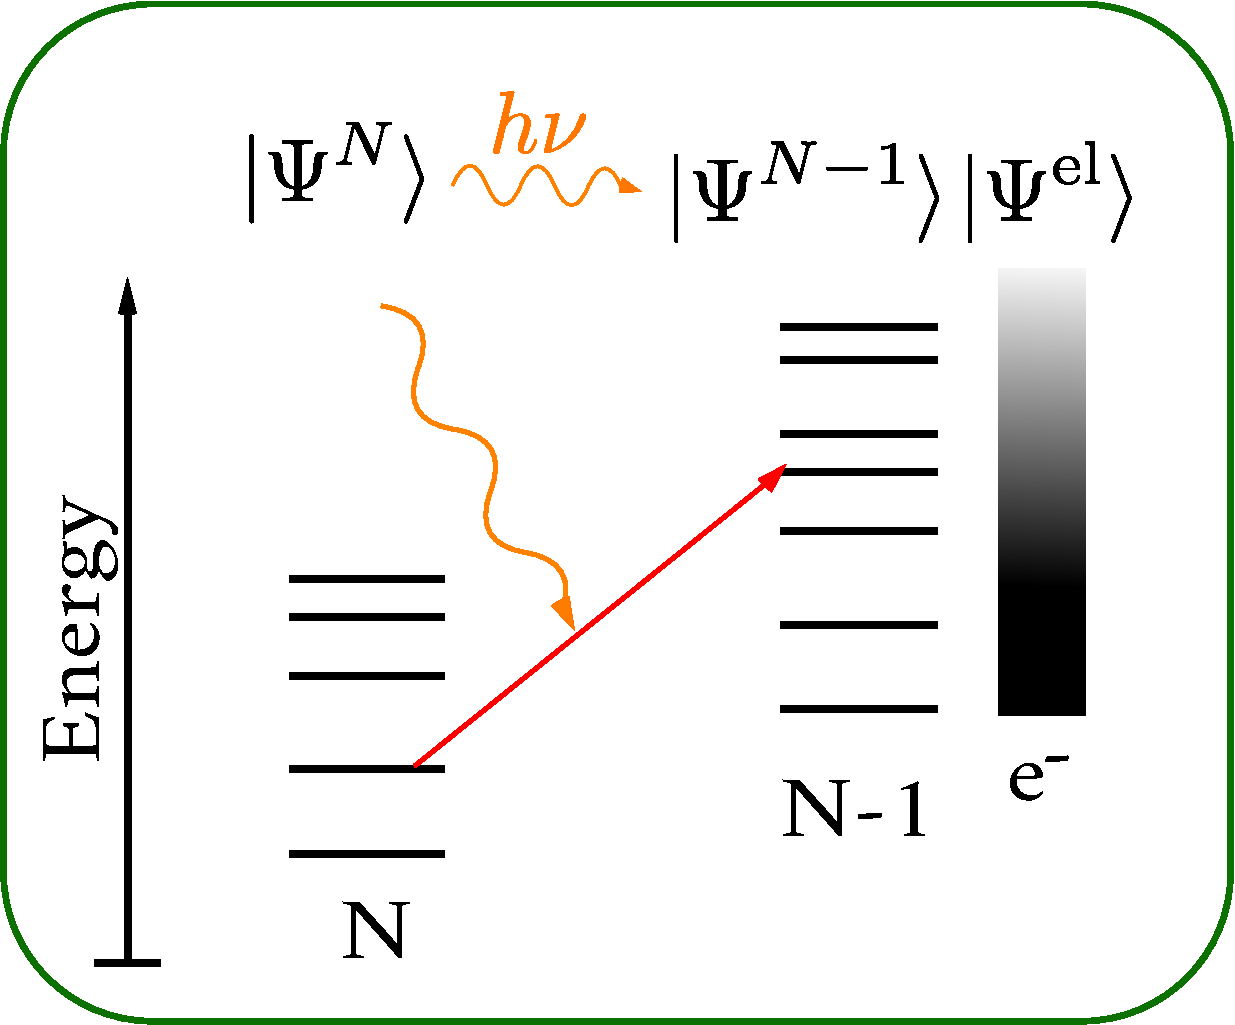
\includegraphics[width=0.61\textwidth]{Figures/PESscheme}
   \caption{Schematic representation of a photoelctron transition : an incoming photon with energy $h\nu$ ionises the $N$-electron system, transfering it into a free electron in a continuum state and a system of $N-1$ bound electrons.
   The bars denote bound states, the color-gradient depicts the energy of the outgoing electron.}
   \label{fig:PESscheme}
\end{wrapfigure}
Furthermore, photoelectron spectroscopy provides a more direct access to the energy levels than optical absorption and emission spectroscopy since the transition energies are obtained with respect to the vacuum level and no ``dark'' states occur due to different selection rules.
Finally the ease of handling changed particles experimentally makes this method appealing and a good temporal resolution can be achieved by varying the path in the time of flight spectrometer.
Moreover, besides its capabilities in steady state spectroscopy, photoelectron spectra are the standard tool to study attosecond physics due to the naturally high energy of the short pulses which ionise the systems under study \cite{as1, as2, as3, as4, as5, as6}.
However, a limitation of photoelectron spectroscopy is that the short free-path of electrons in condensed phases limits the probe depth significantly.

Having performed a measurement of a photoelectron spectrum (PES) it is, at least for complex systems, rich of features and hence the interpretation requires theoretical methods.
This especially applies to systems with strong electron correlation which manifests itself in the appearance of combination transitions.
Over the decades a large variety of methods to calculate photoelectron spectra have been developed at different levels of theory.
In literature often the theoretical spectra are estimated on the basis of Koopmans' theorem \cite{koopmans}, (or its density functional theory (DFT) counterpart \cite{koopmansDFT},) assuming equal intensities for all transitions \cite{OT-RSH,Koerzd1,Koerzd2,Gao_wopperer}.
Even though this is a quite successful approach for solid states \cite{Solid2,Leckey1992} and gives an easy interpretation, it is too simplistic in many cases since it neglects electron relaxation and correlation effects and hence may give an invalid picture as shown by Cederbaum \textit{et al.} even for small systems such as various diatomics \cite{2phcederbaum2, cederbaumN2}.
Furthermore in this model no reliable information about intensities can be obtained.
To retrieve quantitative  transition strengths, more advanced models are needed.
Since simulations in time-domain are very demanding  they are only applied to small molecules, mainly to study strong-field effects such as high harmonic generation \cite{H2pDeCleva,as2,hhg, zhangHHG,dromey_HHG} which can not be described in frequency-domain.
In this thesis however the focus is on complex molecular systems and a wide range of kinetic energies, while more moderate field strengths should be applied.
Hence frequency-domain methods derived from a perturbation theory with respect to the irradiating electromagnetic field are applicable here.

In this thesis, the PESs are calculated within the Dyson orbital (DO) formalism which is derived and explained in more detail.
This formalism is based on Fermis' Golden Rule \cite{fgr} and allows a reduction of the dipole moment matrix element from an $N$-electron integral to effective one-particle quantities. % each for initial and final state.
Thereby the initial state and the bound part of the final state are represented by a one-electron quantity denoted as DO.
The other wave function entering the dipole moment operator is the free electron function (FEF).
In this formalism electron relaxation and correlation effects between bound states of the unionised and ionised systems are included, allowing the description of combination transitions.
Per contra, this formalism neglects the correlation of the outgoing electron with the ionic remainder and thus may neglect certain transitions \cite{LiSonntag}.

Since the bound state wave functions can be obtained from standard quantum-chemical tools, the computation of the DO is straightforward even though technically demanding \cite{MAgg}.
The computation of the FEF is in general not trivial since analytic solutions are known only for few special cases such as hydrogen-like atoms \cite{Lifschitz} and general basis sets as they are used for bound states are not available.
Among others, three analytic expressions have been suggested, each based on an expansion of spherically symmetric functions in plane waves \cite{ezDyson}.
One of them is the spherical wave basis which is a set of solutions of the Schr\"odinger equation (SE) without any potential and hence is especially well-suited for photodetachment from negative ions, leaving systems in an uncharged state \cite{ezDyson, DO_TDDFT}.
The other two expansions are based on Coulomb waves which assume a Coulomb potential and hence are exact for the ionisation of hydrogen-like atoms \cite{Lifschitz}.
Thereby one of them is an expansion in Coulomb waves for the given momentum vector $\vec{k}$ while the other is an asymptotic expression for Coulomb waves with vanishing momentum (Coulomb $|\vec{k}|=0$).
The functions each are expanded in a series of increasing quantum numbers for angular momentum $l$ and its projection $m$.
Since all three functions assume spherical symmetry of the potential, they are expected to give a good approximation to the real FEF for spherically symmetric systems only.
Ionisation \textit{e. g.} from a delocalised orbital of a linear molecule have a different symmetry and thus can be expected to be described only crudely by this approach.
%However, the more the system under consideration differs from spherical symmetry, the larger angular momenta are needed to describe the correct FEF and hence the truncated expansion is expected to give only a poor estimate of the correct function.
The effects due to lower molecular symmetry become especially important for low kinetic energies because the interaction with the ionic remainder becomes strong in this case. 

To analyse the quality of a given expression for a FEF, it is instructive to study the intensity of a given transition as a function of kinetic energy.
Such a study is examined in Figure \ref{fig:Ekin}, showing the intensity of the photoionisation transition from the highest occupied molecular orbital (HOMO) of water for different kinetic energies of the photoelectron, estimated with the above-mentioned expansions.
The comparison shows that all three expansions yield different intensities for most transition energies.
Besides leading a wrong wrong symmetry of the FEF, these expansions yiled even in the limit of infinite terms only a plane-wave, neglecting the ionic potential and hence are not asymptotically correct.

\begin{wrapfigure}{r}{0.62\textwidth}
   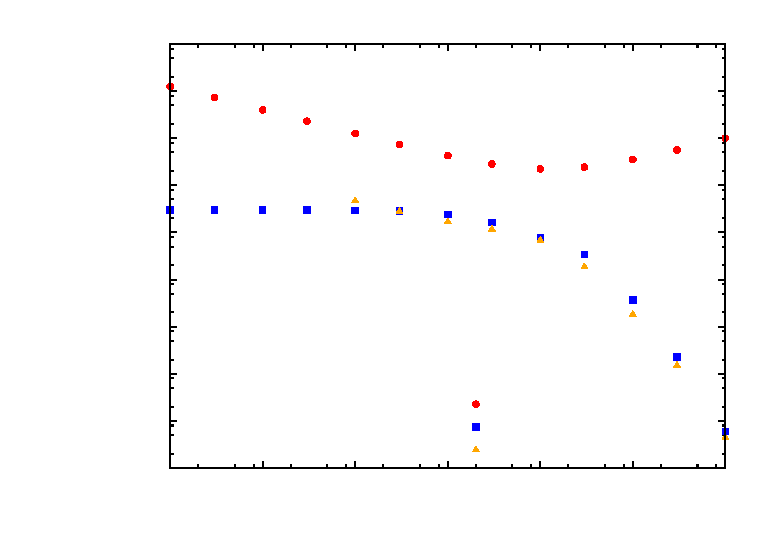
\includegraphics[width=0.61\textwidth]{Figures/water1}
   %\resizebox{\columnwidth}{!}{% GNUPLOT: LaTeX picture with Postscript
\begingroup
  \makeatletter
  \providecommand\color[2][]{%
    \GenericError{(gnuplot) \space\space\space\@spaces}{%
      Package color not loaded in conjunction with
      terminal option `colourtext'%
    }{See the gnuplot documentation for explanation.%
    }{Either use 'blacktext' in gnuplot or load the package
      color.sty in LaTeX.}%
    \renewcommand\color[2][]{}%
  }%
  \providecommand\includegraphics[2][]{%
    \GenericError{(gnuplot) \space\space\space\@spaces}{%
      Package graphicx or graphics not loaded%
    }{See the gnuplot documentation for explanation.%
    }{The gnuplot epslatex terminal needs graphicx.sty or graphics.sty.}%
    \renewcommand\includegraphics[2][]{}%
  }%
  \providecommand\rotatebox[2]{#2}%
  \@ifundefined{ifGPcolor}{%
    \newif\ifGPcolor
    \GPcolortrue
  }{}%
  \@ifundefined{ifGPblacktext}{%
    \newif\ifGPblacktext
    \GPblacktexttrue
  }{}%
  % define a \g@addto@macro without @ in the name:
  \let\gplgaddtomacro\g@addto@macro
  % define empty templates for all commands taking text:
  \gdef\gplbacktext{}%
  \gdef\gplfronttext{}%
  \makeatother
  \ifGPblacktext
    % no textcolor at all
    \def\colorrgb#1{}%
    \def\colorgray#1{}%
  \else
    % gray or color?
    \ifGPcolor
      \def\colorrgb#1{\color[rgb]{#1}}%
      \def\colorgray#1{\color[gray]{#1}}%
      \expandafter\def\csname LTw\endcsname{\color{white}}%
      \expandafter\def\csname LTb\endcsname{\color{black}}%
      \expandafter\def\csname LTa\endcsname{\color{black}}%
      \expandafter\def\csname LT0\endcsname{\color[rgb]{1,0,0}}%
      \expandafter\def\csname LT1\endcsname{\color[rgb]{0,1,0}}%
      \expandafter\def\csname LT2\endcsname{\color[rgb]{0,0,1}}%
      \expandafter\def\csname LT3\endcsname{\color[rgb]{1,0,1}}%
      \expandafter\def\csname LT4\endcsname{\color[rgb]{0,1,1}}%
      \expandafter\def\csname LT5\endcsname{\color[rgb]{1,1,0}}%
      \expandafter\def\csname LT6\endcsname{\color[rgb]{0,0,0}}%
      \expandafter\def\csname LT7\endcsname{\color[rgb]{1,0.3,0}}%
      \expandafter\def\csname LT8\endcsname{\color[rgb]{0.5,0.5,0.5}}%
    \else
      % gray
      \def\colorrgb#1{\color{black}}%
      \def\colorgray#1{\color[gray]{#1}}%
      \expandafter\def\csname LTw\endcsname{\color{white}}%
      \expandafter\def\csname LTb\endcsname{\color{black}}%
      \expandafter\def\csname LTa\endcsname{\color{black}}%
      \expandafter\def\csname LT0\endcsname{\color{black}}%
      \expandafter\def\csname LT1\endcsname{\color{black}}%
      \expandafter\def\csname LT2\endcsname{\color{black}}%
      \expandafter\def\csname LT3\endcsname{\color{black}}%
      \expandafter\def\csname LT4\endcsname{\color{black}}%
      \expandafter\def\csname LT5\endcsname{\color{black}}%
      \expandafter\def\csname LT6\endcsname{\color{black}}%
      \expandafter\def\csname LT7\endcsname{\color{black}}%
      \expandafter\def\csname LT8\endcsname{\color{black}}%
    \fi
  \fi
  \setlength{\unitlength}{0.0500bp}%
  \begin{picture}(7200.00,5040.00)%
    \gplgaddtomacro\gplbacktext{%
      \csname LTb\endcsname%
      \put(1342,704){\makebox(0,0)[r]{\strut{} 1e-05}}%
      \put(1342,1156){\makebox(0,0)[r]{\strut{} 0.0001}}%
      \put(1342,1609){\makebox(0,0)[r]{\strut{} 0.001}}%
      \put(1342,2061){\makebox(0,0)[r]{\strut{} 0.01}}%
      \put(1342,2513){\makebox(0,0)[r]{\strut{} 0.1}}%
      \put(1342,2966){\makebox(0,0)[r]{\strut{} 1}}%
      \put(1342,3418){\makebox(0,0)[r]{\strut{} 10}}%
      \put(1342,3870){\makebox(0,0)[r]{\strut{} 100}}%
      \put(1342,4323){\makebox(0,0)[r]{\strut{} 1000}}%
      \put(1342,4775){\makebox(0,0)[r]{\strut{} 10000}}%
      \put(1474,484){\makebox(0,0){\strut{} 0.001}}%
      \put(2362,484){\makebox(0,0){\strut{} 0.01}}%
      \put(3250,484){\makebox(0,0){\strut{} 0.1}}%
      \put(4139,484){\makebox(0,0){\strut{} 1}}%
      \put(5027,484){\makebox(0,0){\strut{} 10}}%
      \put(5915,484){\makebox(0,0){\strut{} 100}}%
      \put(6803,484){\makebox(0,0){\strut{} 1000}}%
      \put(176,2739){\rotatebox{-270}{\makebox(0,0){\strut{}Intensity [arb. u.]}}}%
      \put(4138,154){\makebox(0,0){\strut{}E$_	ext{kin}$ [eV]}}%
    }%
    \gplgaddtomacro\gplfronttext{%
      \csname LTb\endcsname%
      \put(3982,1317){\makebox(0,0)[r]{\strut{}Coulomb ($|vec{k}|=0$)}}%
      \csname LTb\endcsname%
      \put(3982,1097){\makebox(0,0)[r]{\strut{}spherical}}%
      \csname LTb\endcsname%
      \put(3982,877){\makebox(0,0)[r]{\strut{}Coulomb}}%
    }%
    \gplbacktext
    \put(0,0){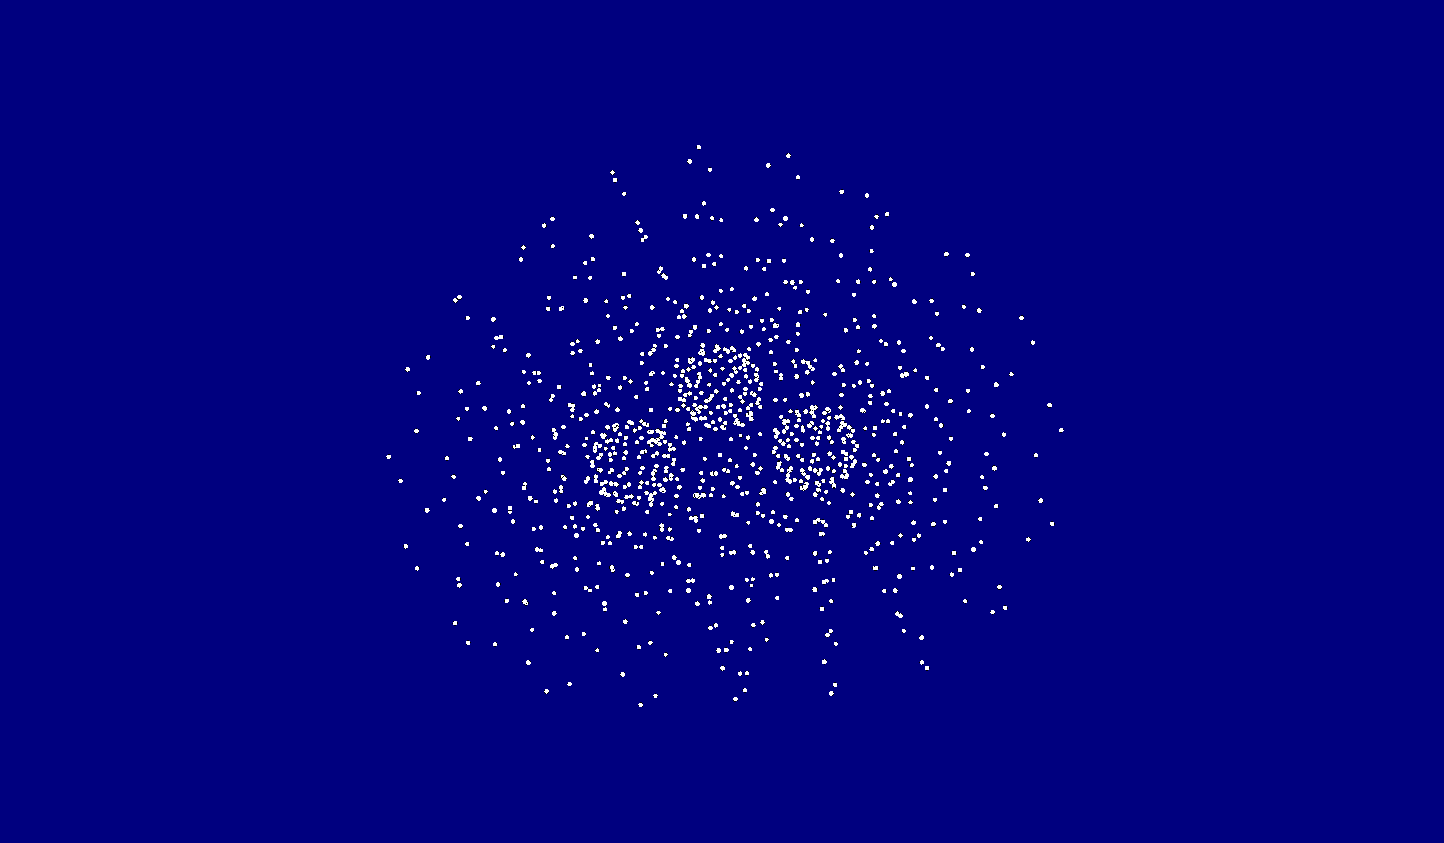
\includegraphics{water1}}%
    \gplfronttext
  \end{picture}%
\endgroup
}
   \caption{The intensity of the lowest-lying transition of water depending on the kinetic energy of the photoelectron. Each expansion is performed up to $l=10$.} 
   \label{fig:Ekin}
\end{wrapfigure}
To overcome the restrictions in symmetry and kinetic energy of the photoelectron function, an explicit formulation is needed, taking the molecular electrostatic potential experienced by the outgoing electron into account.
%To account for the exact electrostatic potential, the final state needs to be treated as a full $N$ electron system to account for the correlation effects.
Assuming that the correlation between the FEF and the bound states of the ion is weak (which is a prerequisit for the DO formalism anyway), one can use the mean-field potential of the molecular remainder.
This allows for obtaining the FEF from the one-electron SE with an appropriate potential and thus reduces the complexity compared to the exact case where a coupled $N$-electron equation needs to be solved, considerably.

In the thesis at hand a good approximation to the FEF is aimed which should be applicable to a wide range of molecules and photon energies.
Such a flexible description is possible exploiting the finite element method for solving the SE.
In the finite element method, the space of interest is subdivided into small volume elements and solved variationally with stepwise polynomials whose support spans over one or few elements only \cite{femBraess,femGilbarg}.
The finite element description is especially efficient here since the size of the elements can be locally adapted to reproduce finer structures or broader shapes \cite{femBraess,femCiarlet}.
Using finite elements, the one-particle SE is formulated a generalised eigenvalue problem with sparse matrices.

An important characteristic of the exact FEF is its spacially infinite extend which can not be handled by the finite element method.
To describe the function in a good approximation, the finite elements are extended by infinite elements \cite{astley3, astley2, Astley,dreyer} which are volume elements with infinite radial extend that are connected to the outer surface of the finite element region.
Thereby the radial function is a polynomial in $\frac 1r$ multiplied by $e^{ikr}$, resembling the asymptotic behaviour of known analytic solutions and fulfilling the Sommerfeld radiation condition \cite{sommerfeldCond}.

%The bound states can be obtained on the level of density functional theory (DFT) which is a formally exact method and yields a quadratic scaling with the number of electrons compared to the exponential growth of the SE \textcolor{green}{source}.
%The DFT is based on the Hohenberg-Kohn theorems \cite{HohenbergKohn}, stating that the total electron density contains all information to obtain any system property.
%However, the correct form of the exchange potential as well as the kinetic energy are not known therein and hence approximate functionals need used.
%While the kinetic energy can be estimated reasonably by the Kohn-Sham scheme \cite{KohnSham}, the expressions used for the exchange-correlation potential yield electron densities that have a wrong long-range asymptotic behaviour which affects the observables of these systems \cite{Koerzd1, Koerzd2, Bokareva}.
%To reduce this error, range-separated hybrid functionals are used where the usual DFT exchange functionals are used at close distances while a Hartree-Fock exact exchange ensures the correct behaviour at larger distances.
%Thereby the interchange between these contributions is modelled via an error function with a characteristic distance that is optimized for each system separately.
%This procedure has been observed to enhance the accuracy of the predicted properties such as the orbital energies \cite{Bokareva,GrellKuehn, Gerber, Gerber2}.
The bound states can be obtained on the level of density functional theory (DFT) which is a formally exact method based on the Hohenberg-Kohn theorem \cite{HohenbergKohn}, stating that the total electron density determines all system properties such as electronic binding energies.
However, the correct form of the exchange potential as well as the kinetic energy are not known as functionals of the electron densety and hence approximate functionals need used.
While the kinetic energy can be estimated reasonably by the Kohn-Sham scheme \cite{KohnSham}, the expressions used for the exchange-correlation potential yield electron densities that have a wrong long-range asymptotic decay which affects the observables of these systems \cite{Koerzd1, Koerzd2, Bokareva}.
To reduce this error, range-separated hybrid functionals are used where the usual DFT exchange functionals are used at small distances while a Hartree-Fock exact exchange ensures the correct behaviour at larger distances.
The interchange between these contributions is modelled via an error function with a characteristic distance that is optimized for each system separately.
This procedure has been observed to enhance the accuracy of the predicted properties such as the orbital energies \cite{Bokareva,GrellKuehn, Gerber, Gerber2}.

While the schemes described above are well established, their combination is only rarely used.
Especially the FEF is found in literature to be approximated only crudely as plane-wave functions \cite{planeWave} or in some expansion as described above \cite{ezDyson,MAgg,GrellKuehn}.
The goal of this thesis is to use the DO formalism with bound states being described by DFT using the above-mentioned optimized range-separated hybrid (OTRSH) functionals to obtain accurate orbital energies and complement it with a FEF that accounts the molecular electrostatic potential explicitly using the finite and infinite element methods which have been applied only to very few quantum mechanical problems \cite{sobaMolecule,bettessHarmonic}.

%The Dyson formalism is well established and has been shown to give reasonable quantitative agreement with experiment for many different systems \cite{ezDyson,DO_TDDFT,bawagan,hafied}.
%In the protocol used the DO is calculated using density functional theory (DFT) and its time-dependent counterpart with a locally modified version of \prog{NWChem} \cite{nwchem} and the \prog{Gaussian 09} package \cite{g09}.
In the protocol used the DFT and time-dependent DFT calculations for excited states are done using a locally modified version of \prog{NWChem} \cite{nwchem} and the \prog{Gaussian 09} package \cite{g09}.
From those, the DO is calculated with the in-house code \prog{DYSON} developed previously \cite{MAgg}.
A self-written interface extracts the required data as \textit{e.g.} the molecular orbital coefficients and overlap matrix of atomic orbitals from the output of these programs.
For the computation of the FEF, the grogram \prog{FreeWilly} \cite{FreeWilly} is developed using the finite element library \prog{Libmesh} \cite{libmesh}. 
\prog{Libmesh} is an open source library that provides a broad range of capabilities and interfaces to several high-performance linear algebra libraries \cite{slepc1,slepc2,petsc}.
Moreover, it supports MPI parallelisation and implements a recent formulation of the above-mentioned infinite elements \cite{dreyer}.
Especially the latter is to the best of my knowledge a unique option.
Furthermore it has an automated procedure to adaptively refine or coarsen the elements according to local error estimates.

Tho goal of this thesis is to find a systematic way to setup the finite element mesh for any given molecule to describe the photoelectron with a reasonable accuracy that goes beyond the capabilities of existing programs in this field.
%Moreover, the molecular electrostatic potential is to be obtained in the region of interest, requirering some modification in the code of \prog{NWChem} and a three-dimensional interpolation scheme that can handle nonuniform data.
%Finally, to obtain the dipole matrix elements, the DO has to be projected onto the space of finite elements.
%Therfore the explicit function is obtained by evaluating the basis functions at given quadrature points.
The developed protocol is applied to seval systems.
To show the properties of the respective setup and compare different schemes suggested, atomic hydrogen is used for which an analytic solution, namely the Coulomb waves, is known.
Further tests are applied to lithium, \textcolor{red}{doing .... and Cross section}.
As a simplet test-system for a molecular case  carbondioxide is chosen for which several experimental as well as theoretical reference-data are available, \textcolor{red}{studying the PES and croos section}.
For this system, the usual approach to represent the FEF as a Coulomb wave is expected to be not valid.
Finally, as a representative for larger and more complex molecules, here benzene is chosen which is a well-studied system.


\chapter{Calculation of Photoelectron spectra}
%lit. survey I
\label{ch:calcPES}
The large variety of systems and effects studied with photoelectron spectroscopy led to the existence of diverse methods for theoretical modelling of the spectra \cite{PESbook, x-ray}.
In this work, the focus is put on steady-state photoelectron spectra of molecular systems with a size up to some tens of atoms.
As light source, here a classical ultra-violet or soft X-ray source with a discrete spectrum such as a gas discharge lamp or a laser is assumed where the strength of the applied electromagnetic field is weak and the kinetic energy of the outgoing electrons reaches at most tens of electronvolt but may become arbitrarily small.

A summary of methods that can be used to describe the most important scenarios arising in photoelectron spectroscopy is given in the Table \ref{tab:PEScat} and some of them are described in more detail in the following sections.
The main classification of these methods can be done dividing them into time and frequency domain.
These domains are related to each other via the Fourier transform but provide different pictures and properties.
Using a frequency-domain method, the Hamiltonian has to be diagonalised to obtain the states' energies and wave functions.
In contrast to this, in time domain the Hamiltonian is applied to an initial state to propagate the system in time.
Usually such a simulation needs several thousands of propagation steps to obtain reasonable accuracy.
Moreover, the joint treatment of bound and continuum states demands a large and flexible basis which makes time domain methods usually computationally very demanding and restricts their applicability to small systems as shown in the Table \ref{tab:PEScat}.
On the other hand, in frequency-domain the nonlinear response properties are neglected so that strong-field effects such as multiphoton ionisation and high harmonic generation (HHG) can not be treated.
Due to the different treatment of the system in both domains, they each have a set of methods that can be used and which are more or less specific to the domain as shown in the third column of Table \ref{tab:PEScat}.
The same holds for the quantum chemical methods available to treat the system.
\begin{table}
\begin{tiny}\begin{tabular}{|c|c|c|c|c|c|}
\hline
                 & Field Str. & Method & System Size & Typical Problems &  QC$^{(a)}$ \\
\hline
\begin{tabular}{c}Time-\\ domain  \end{tabular}   &
        \begin{tabular}{c} weak to \\ strong \end{tabular} & 
        \begin{tabular}{c} TDDO \cite{TD-do}\\ SE \\ Green's function \end{tabular} &
        \begin{tabular}{c}atoms \cite{bauch1}, \\ diatomics \cite{bauch2,H2pDeCleva,saPonzi}\\ triatomics \cite{radau} \end{tabular} & 
        \begin{tabular}{c}HHG \cite{hhg,zhangHHG,dromey_HHG}, \\Multiph. ionisation \\ attosec. dynam.\cite{as1,as2,as3,as4,as5,as6} \end{tabular} &
        \begin{tabular}{c}(TD)DFT, \\GASCI \cite{bauch1}, \\ EOM-CC \cite{CAPccEOM},\\ CASSCF \end{tabular} \\
\hline
\begin{tabular}{c}Frequency-\\ domain \end{tabular} & 
        weak & 
        \begin{tabular}{c} R-Matrix \cite{Li-R,Li-R1,Burke,r-mat,R-mol1}\\ DO \cite{planeWave,DO_TDDFT} \\Green's Function \cite{GreenBayse,2phcederbaum} \\ Koopmans'\cite{dos,dos2,koopmansDFT} \end{tabular} &
        \begin{tabular}{c}up to \\biomolecules \cite{bioPES}, \\ solid state \cite{Solid2,Leckey1992} \end{tabular}& 
        \begin{tabular}{c} steady-state, \\ angle-res. PES \\time-res. PES \end{tabular}& 
        \begin{tabular}{c} RASSCF \cite{MAgg,GrellKuehn}, \\ TD-DFT \end{tabular} \\
\hline
\end{tabular} \end{tiny}
\caption{Overview of time- and frequency-domain methods and theyr typical applications.\\
  \small{$^{(a)}$QC: quantum chemical; GASCI: generalised active space configuration interaction; CASSCF: complete active space self-consistent field; EOM-CC: equation of motion- coupled cluster; RASSCF: restricted active space self-consistent field}.}
\label{tab:PEScat}
\end{table} 
%These nonlinear effects however usually do not play any role for classical light sources such as gas discharge or heat lamps and even most non-pulsed lasers.

Besides the distinction according to the domain, the methods can be also categorised according to the partitioning of the system they use which is sketched in Figure \ref{fig:PEScat}.
\begin{wrapfigure}{r}{0.7\textwidth}
   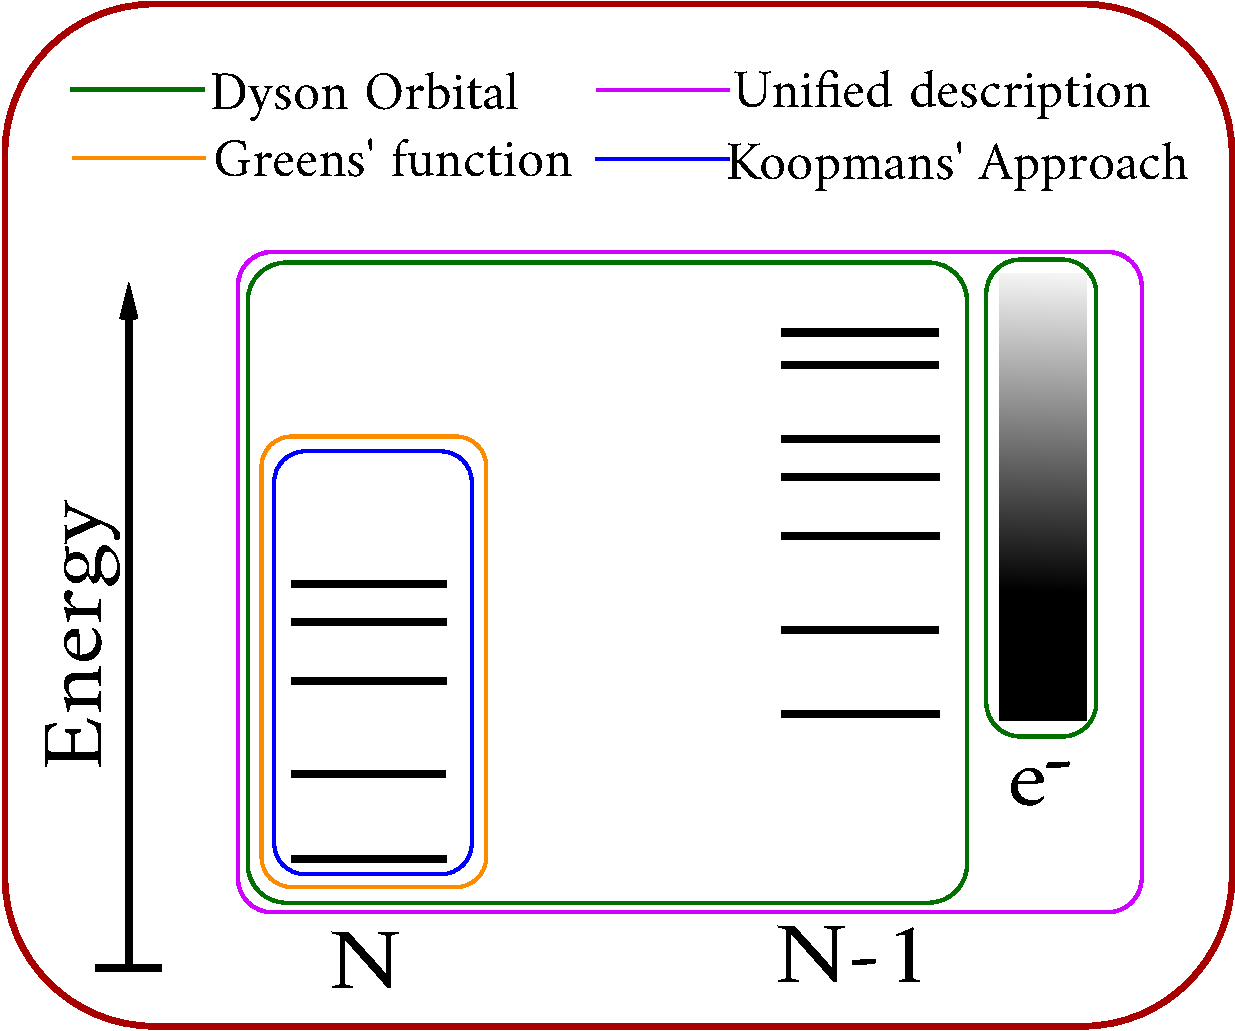
\includegraphics[width=0.7\textwidth]{Figures/Methods}
   \caption{Scheme of the system-representation used in the different methods.}
   \label{fig:PEScat}
\end{wrapfigure}
The simplest and crudest method is an approach derived from Koopman's theorem where only the ground state of the un\-ion\-ised state is considered which is visualised in Figure \ref{fig:PEScat} by the fact that the box for this method is only at the $N$-electron system.
Similarly, also the Green's function approach treats only the initial state but accounts for electron relaxation and thus correlation effects during ionisation due to its quasi-particle picture.
In the DO formalism, in contrast, the final state is treated explicitly, using a partitioning into the bound $N-1$-electron state $|\Psi^{N-1}\rangle$ and the FEF $|\Psi^\text{el}\rangle$.
%The wave function of the initial state $|\Psi^{N}\rangle$ moreover is obtained in a separate calculation; so in total three different calculations are used which is represented by the three boxes in Figure \ref{fig:PEScat}.
Finally a large class of methods treat the system uniformly, using a joint treatment for the bound and continuum states as indicated by the single box in Figure \ref{fig:PEScat}.
%Typically time-domain methods are in this last group of methods.

The Koopmans' approach is, at least among the frequency domain methods, the most prominent representative \cite{Koerzd1,PottsHolland,dos,dos2}.
In this scheme, the systems ground state is computed with a self-consistent field quantum mechanical method to obtain the one-electron binding energies.
The photoelectron spectrum is than estimated using the orbital energies as the transition energies and using uniform intensities.
Although this method has shown to be in qualitative agreement with experiments for different systems \cite{Koerzd1,Koerzd2, EggerKronik,PottsHolland,YepesJaque}, it breaks down in case of strong electron correlation \cite{2phcederbaum,2phcederbaum2} due to relaxation of the orbitals upon ionisation.
%Since the estimation of the role of correlation effects can only hardly be estimated in advance, this method has only poor predictive character.
This method is characterised by its low computational costs and robustness and, thus, is well-suited for very large systems such as solid state problems where calculations beyond ground-state DFT are very demanding or not feasible at all.

In the following sections, the most important methods will be briefly introduced according to their affiliation to the groups distiguished in Figure \ref{fig:PEScat}.
First, in section \ref{ch:gf} the working equations of the Green's function approach are introduced to give a fundamental understanding of this group of methods.
Thereafter, in section \ref{ch:r-mat} several approaches both in time- and frequency-domain are described that use a unified descrption of the complete $N$-electron system.
Finally the DO formalism is derived in more detail, since it is the method of choise in this work, in section \ref{ch:do}.

\section{The Green's Function Approach}
\label{ch:gf}
From a formal point of view, the computation of photoelectron spectra using the Green's function approach is similar to the use of Koopmans' approach since in both methods only the ground state of the unionised system is considered.
However, the level of theory achievable when using Green's functions is much higher.

In contrast to most other quantum-chemical methods, in the Greens' function approach expectation values for a given operator $\hat{O}$ are not computed as a scalar product $\langle \Psi^N |\hat{O} | \Psi^N \rangle $ with the wave function $|\Psi^N\rangle$ of the $N$ electron state of interest, but by contour integrals with the Greens' function \cite{bookGF, 1pGFcederbaum}.
Thereby the (one particle) Greens' function is a matrix $\mat{G}$ whose elements are defined as
\begin{equation} \label{eq:defGF}
G_{i,j}(t,t')= -\text{i}\langle \Psi^N | \hat{T}\left(\hat{a}_i(t)\hat{a}_j^\dagger(t')\right)|\Psi^N\rangle 
\end{equation}
with the creation operator $\hat{a}^\dagger_j (t)=e^{\text{i}\hat{H}t}\hat{a}^\dagger_j e^{-\text{i}\hat{H}t}$ of an electron in state $j$ at time $t$ in Heisenberg picture and the annihilation operator $\hat{a}(t)=e^{-\text{i}\hat{H}t}\hat{a}_j e^{\text{i}\hat{H}t}$ respectively.
$\hat{T}$ is the Dyson time ordering operator that orders the operators $\hat{a}$ and $\hat{a}^\dagger$ by their time arguments to ensure that the operator with smaller time argument acts first \cite{bookGF}.
Hence, the Greens' function can be interpreted as an additional electron (or hole, depending on the time ordering) propagating from $t'$ to $t$ in a system described by the Hamiltonian $\hat{H}$ \cite{bookGF}.

%In this approach the calculation of photoelectron spectra is formulated such that the poles and residues of the Fourier transformed Greens' function are searched.
%This becomes clear when writing the time-ordering operator in equation (\ref{eq:defGF}) explicitly
To find an expression of the Green's function (\ref{eq:defGF}) from which the transition energies and intensities can be extracted, it needs to be reformulated.
In the first step, the time ordering operator is written explicitly which results in 
\begin{equation} \label{eq:GF}
G_{i,j}(t,t')= \text{i}\langle \Psi^N | \hat{a}_j(t)\hat{a}^\dagger_i(t') |\Psi^N\rangle \Theta(t-t') -
                   \text{i} \langle \Psi^N | \hat{a}^\dagger_i(t')\hat{a}_j(t) |\Psi^N\rangle \Theta(t'-t).
\end{equation}
Inserting the closure relation $\hat{1}=\sum_k |\Psi^M_k\rangle\langle \Psi^M_k |$, where $M=N\pm 1$ and $|\Psi^M_k\rangle$ describes a bound state, between the operators in both terms of (\ref{eq:GF}), the Lehmann representation \cite{bookGF} is obtained whose Fourier transform is
\begin{equation}\label{eq:gfSpect}
G_{i,j}(\omega)=\text{i} \sum_k\frac{\left|\langle \Psi^N | \hat{a}_j|\Psi^{N+1}_k \rangle \right|^3}{\omega-(E_k^{N+1}-E^N)+\text{i}\nu}-
                \text{i}\sum_k\frac{\left|\langle \Psi^N | \hat{a}^\dagger_i|\Psi^{N-1}_k \rangle \right|^2}{\omega+(E_k^{N-1}-E^N)-\text{i}\nu},
\end{equation}
where $\nu$ is a small parameter arising from calculation of principal value and $\omega$ denotes the argument of the Fourier transform while $E^N$ and $E_k^M$ are the energies of the $N$-electron ground stated $|\Psi^N\rangle$ and of the $k$-th $M$-electron state $|\Psi_k^M\rangle$, respectively.
In this form, the second sum corresponds to transitions in the PES: the nodes of the denominator (poles of the Greens' function) can be easily assigned to the ionisation potentials and, thus, the transition energies in photoelectron spectra.
Further, the integrals in the nominator are equivalent to the sudden approximation derived in chapter \ref{ch:sa} and hence provide a good approximation to the transition strengths.
The terms in the first sum correspond to the respective quantities of electron detachment \cite{1pGFcederbaum}.

However, computing the Greens' function is a demanding task which is of similar complexity as the computation of a solution to the SE.
Over the years several approaches were developed of which the algebraic diagrammatic construction \cite{1pGFcederbaum} and the equation of motion \cite{PottsHolland,1pGFcederbaum} are the most prominent.
In the diagrammatic construction one starts with an initial zeroth order Greens' function $\mat{G}^0(\omega)$ constructed in a Hartree-Fock basis and corrects it iteratively by the term $\mat{G}^0(\omega)\mat{\Sigma}(\omega)\mat{G}(\omega)$, where $\mat{\Sigma}(\omega)$ is the self-energy, an effective potential that is used to recover electron correlation and relaxation effects \cite{GreenBayse}.
The self-energy usually is expanded in a perturbation series with respect to Feynman diagrams with increasing number of vertices and is exact in the limit of infinite terms \cite{bookGF,cederbADC}.
The one-particle energies, Coulomb matrix elements and overlap integrals are obtained from self-consistent field (SCF) calculations \cite{1pGFcederbaum} \textit{e.g.} on the HF-level \cite{GreenBayse} but (TD)DFT or any other quantum chemical method can be used as well via the GW-approach \cite{gf_intro,hedinGW}.
Being much easier to compute, the Hartree-Fock basis has the disadvantage that only single configurational electronic states can be treated.

On the other hand, an important advantage of the Greens' function method is that the transition energies are computed directly whereas in most other methods they are calculated as the difference of the initial and final state energies.
The latter approach however can lead to errors in the electronvolt range when the difference in the correlation energy is badly estimated \cite{1pGFcederbaum}.

%Another, yet similarly simple approach used in cases where only few electronic transitions are present is to fit the intensity to experimental data \cite{winterWater,hemberg1}.
%This is especially used when the vibrational structure is resolved.
%
%Here, two different approaches are possible.
%While most methods use Fermis Golden Rule 
%\[  \sigma(\omega)\propto |\langle |\hat{mu}|\rangle|^2 g(E_f-E_i+h\nu -\omega)
%\]
%where the intensity of the transitions is calculated via the dipole matrix elements, the other route is
%via the complex polarisability $\alpha(\omega)=\int_{IP}^\infty \frac{df(\epsilon)}{\epsilon^2-\omega^2}$. 
%In the latter case, the spectrum is obtained via
%\[ \sigma(\omega)=\frac{4\pi \omega}{c} Im(\alpha(\omega)).\]
% Some of them are especially generated for special geometries such as the R-matrix method described in chapter \ref{ch:r-mat}, others such as the Greens' function or Dyson orbital formalism introduced in the chapters \ref{ch:gf} and \ref{ch:do} respectively are more general but can not reach the same accuracy.
% Besides different classes of molecules, also the light irradiation considered can differ: Some methods are especially designed for large intensities \textcolor{green}{sources} or kinetic energies in the relativistic regime \textcolor{green}{source}.
 %In this work, however, only methods applicable in more moderate regimes are considered, meaning that perturbation theory is applicable and the kinetic energy of the photoelectron is considered to not above the $keV$-range.
%\section{Methods where electron is treated in same footing as bound states}
%\section{Methods with Unified Description of Bound and Free States}
\section{Combined Bound and Continuum State Representation}
\label{ch:r-mat}
%Another large class of methods for computing photoelectron spectra uses perturbation theory in frequency domain or the dipole autocorrelation function in time domain respectively.
%In frequency domain thereby the initial state and final state are described therein each as $N$ electron systems with a uniform scheme, requiring the basis set to be formulated general enough to represent bound as well as free states.
In contrast to the Greens' function method, in which the explicit description of the FEF  omitted, a large group of methods describes the full $N$-electron system before and after the ionisation, respectively (see Figure \ref{fig:PEScat}).
In this section a selection of such methods is presented.
The treatment of bound and continuum states, however, requires a very flexible formalism whose large computational costs restrict its applicability to small systems that often fulfil certain symmetry-requirements and have a small amount of electrons.

The most prominent representative of this class in frequency domain is the R-matrix method \cite{r-mat, r-mat2,Burke}.
Its general idea is to conduct a partition of space into regions which are treated differently and connected by explicit boundary conditions to ensure smoothness of the wave function.
These regions are constructed with concentric spheres, restricting the symmetry of wave functions in this scheme.
Nonetheless it is found to be applied not only to atoms \cite{Li-R,Li-R1,Li-R2} but also to small molecules \cite{R-mol1,R-mol2}.
In the R-matrix formalism the inner region is chosen large enough to contain the bound part of the $N$-electron function that is usually represented by a configuration interaction (CI) expansion of Slater determinants (SDs), using a linear combination of atomic orbitals (LCAO) basis or a grid representation \cite{Burke}.
The FEF is commonly described by a linear combination of bound orbital type functions and continuum functions such as Coulomb waves \cite{r-mat, r-mat2}. %or a product description of spherical Harmonic and a spline-based radial function.
%a antisymmetrised product of Coulomb type wave function with ...\cite{r-mat,r-mat2}.
\begin{wrapfigure}{r}{0.48\textwidth}
   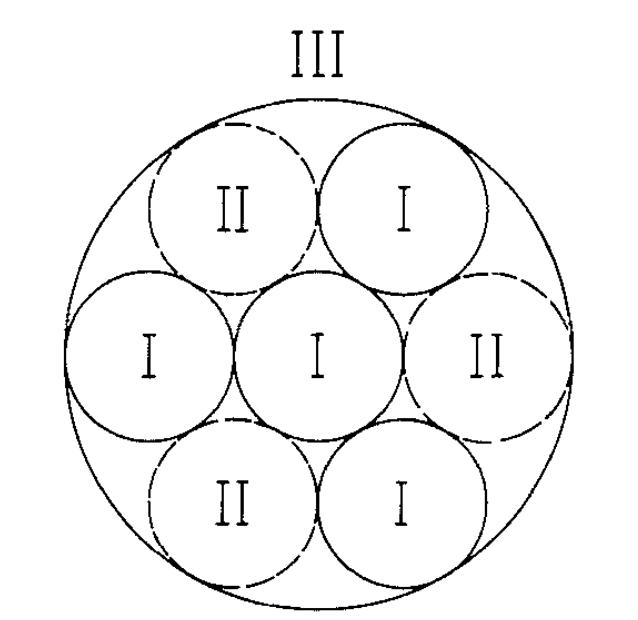
\includegraphics[width=0.48\textwidth]{Figures/JohnsonSpheres}
   \caption{Schematic view of the space partition scheme used by Johnson for a four-atomic molecule:
    I: atomic, II: interatomic and III: outer region \cite{johnson}.}
   \label{fig:johnson}
\end{wrapfigure}
In the outer region, an expansion in Coulomb waves is used to ensure the asymptotically correct behaviour.
In addition to the inner region and the asymptotic outer region further intermediate regions can be added  where the FEF is represented by a multipole-radiation expansion which is a polynomial of inverse powers of the distance to the centre \cite{Burke}.

%in which the multipole functions can be added\cite{Burke}.
A generalisation to non-spherical systems is employed, \textit{e.g.}, by Johnson \cite{johnson} who used different kinds of non-concentric spheres.
One set spheres is centred at atoms while others are placed in the interatomic regions such that the space is filled as dense as possible as shown in Figure \ref{fig:johnson} for a molecule with four atoms.
Each atom is located in the centre of a circle denoted as I while the circles II fill the interatomic space.
An outer sphere surrounds the molecule to account for the asymptotic region similar to the asymptotic region in R-matrix theory.
In this scheme, the exchange-correlation is treated on an approximate level \cite{slaterJohn} and is spherically averaged, resulting in a description that is equivalent to the muffin-tin potential which is a well-known model in solid state physics \cite{MufTin,MufTin1}.
The continuity of the wave-functions as well as their derivatives is ensured over the regions via multiple-scattered-wave theory \cite{johnson}.
%Thereby the potential energy contains besides the Coulomb term also a statistical approximation of the exchange correlation of the form
%\begin{equation}
 %V_{x\alpha}(\vec{r}) = -6\alpha\left( \frac 38 \pi \rho(\vec{r})\right)^{\frac 13} 
%\end{equation}
%where $\rho(\vec{r})$ is the electron density and $\alpha$ is a parameter that is chosen differently for each element.
%In each of the regions the potential %energy is expanded in a superposition of spherical harmonics that is truncated after the $l=0$ term which is equivalent to the muffin-tin potential which is well-known especially for solids \cite{MufTin,MufTin1}.
The wave-functions are chosen in each region as a one-centre expansion in spherical coordinates of the form
\begin{equation} \label{eq:radSE}
\Psi(r, \theta, \phi) =\sum_{l=0}^{l_\text{max}}\sum_{m=-l}^l c_{l,m} R_l(r) Y_l^m(\theta, \phi)
\end{equation}
where $r,\theta,\phi$ are the spherical coordinates and $Y_l^m(\theta,\phi)$ are the spherical Harmonics \cite{Lifschitz} and the radial function $R_l(r)$ is a solution of the radial SE 
\begin{equation} \label{eq:radSEeq}
\frac{\partial^2 R(r)}{\partial r^2} + \left( E-V(r) + \frac{l(l+1)}{r^2} \right)R(r)=0
\end{equation}
with the respective spherically averaged potential $V(r)$ \cite{johnson}.

%A similar approach is to describe the bound and free states at the same level as applied by DeCleva \textit{et al.}  $H_2^+$\cite{H2pDeCleva}.
An approach applied by DeCleva \textit{et al.} to $H_2^+$ \cite{H2pDeCleva} and benzene \cite{DeClevaBenzene} refrains from the use of spheres, allowing for more general boundaries between the inner and outer regions.
Here the FEFs are globally represented as the one-centre expansion (\ref{eq:radSE}) where $R(r)$ is expressed by a B-spline basis. % (details about the spline description are given in section \ref{ch:dvr}).
An advantage of the spline-based description is that smoothness at the interface between the regions is ensured intrinsically.

Another scheme in frequency domain is used by Richards and Larkins \cite{richardsFD} with a hybrid ansatz: The bound states of the H$_2$ molecule are described in the common LCAO scheme and the FEF is described by the product ansatz $\Psi(\vec{r}) = R(r,\theta) e^{im\phi}$, which is a generalisation of (\ref{eq:radSE}), where $R(r,\theta)$ is obtained from a two-dimensional SE on a regular grid using a finite difference (FD) scheme.
In contrast to the previously described methods, here no partition of space is performed but instead a finite box with Dirichlet boundary conditions is used.
Moreover, the FEF is treated on the HF-level, neglecting correlation effects \cite{richardsFD}.

Similar descriptions are used in time domain by several authors \cite{CAPccEOM, bauch1, taoDVR}.
Even though they are much more demanding than calculations in frequency domain, time domain methods can predict strong-field effects and are used to simulate attosecond dynamic which is both not achievable using frequency-domain methods.

An important difference between time- and frequency-domain methods of practical use is that in time-domain unbound particles are described by a wave packet and hence as a localised function.
Moreover, at short times after ionisation the continuum states often can be assumed to be of similar spacial extend as bound states, allowing the basis to be a linear combination of bound state functions but having a complex energy whose real part introduces oscillations and the imaginary part damps the wave function, leading to a finite lifetime of the function \cite{CAPccEOM}.
Moreover a complex absorbing potential (CAP) (discussed in chapter \ref{ch:cap} in more detail) is most often applied, ensuring that the continuum states can be described by bound-state functions by cutting off that part of the wave function which is not localised at the molecule anymore.
Due to these considerations the LCAO basis can be used for the description of the free particles as well, see \textit{e.g.} Jagau \textit{et al.} \cite{CAPccEOM}.
In other simulations, grid-based descriptions are chosen using symmetry-adapted coordinate systems \cite{radau,jacobi, hyperspheric,taoDVR}, allowing for a product ansatz similar to (\ref{eq:radSE}) and hence a reduction in dimensionality.
%In other simulations, a grid-based description is chosen using spherical, elliptical or hyperspherical coordinates, allowing ng for a product ansatz and hence a reduction to one dimension.
On the remaining one-dimensional grids often a discrete variable representation (DVR) (described in section \ref{ch:dvr} of this thesis) is chosen.
As an example, Yip \textit{et al.} \cite{yipDVR} simulate double ionisation of atomic beryllium in spherical coordinates, using the expansion (\ref{eq:radSE}) where $R(r)$ is separated into two regions in which a DVR and a finite element DVR (FE-DVR) scheme are used respectively.
As other examples, Tao \textit{et al.} \cite{taoDVR} as well as Bauch \textit{et al.} \cite{bauch1, bauch2} use the FE-DVR basis in spheroidal coordinates.

The examples introduced above represent only a small fraction of the methods used to describe photoionisation in frequency and time domain.
But a drawback that is common to these methods is that a large number of continuum functions is required which are correlated with the bound electrons and thus lead to a computationally expensive description of the system.
To overcome this drawback, in the DO formalism that is presented in the coming section the description of bound and continuum states is separated into separate problems.

%\textcolor{red}{This is by far not a complete list; are these at least the most important methods?}
%
%A different technique is used by Son \textit{et al.} who use time dependent density functional theory (TDDFT) based on a finite volume scheme instead of the usual LCAO approach.
%Thereby no asymptotic region is utilised, instead the region of interest is chosen by setting a sphere with a given radius around each atom \cite{Son_Chu0,Son_Chu}.

%Sato \textit{et al.}\textcolor{green}{sources} 
\section{The Dyson Orbital Formalism}
\label{ch:do}
The Dyson orbital (DO) formalism can be considered as an approximation to the methods described above.
Here the free and bound states are described separately, see Figure \ref{fig:PEScat}, using a product ansatz.
Using such a separation leads to a neglect of correlation effects between the outgoing electron and the bound states and is often denoted as sudden ionisation limit \cite{ezDyson,MAgg}.
Moreover, non-linear effects as well as recombination transitions are not considered within DO theory.
An important advantage, however, is that the overlap between the initial state and the bound part of the final state is formulated as a one-electron quantity, called DO which can be used to simplify the description of the photoionisation process.
%reducing the computation of the dipole matrix elements to a one-electron integration.
Usually the DO scheme is considered in the frequency domain, but a time domain formulation exists as well and is described in the following section \cite{TD-do}.
%The DO therein can be interpreted as a quasi-particle that is removed from the molecules; incorporating multi-particle effects such as electron relaxation or instantaneous excitation of other electrons.

\subsection{Time-dependent Dyson Orbitals}
%There are several approaches towards Dyson orbitals.
%Here we will mainly follow the derivation of Gritsenko \textit{et al.} \cite{TD-do}, starting from an exact time-dependent expression.
%Here we will mainly follow the derivation of Gritsenko \textit{et al.} \cite{TD-do}, starting from an exact time-dependent expression.
%Thereby the $j$-th time dependent Dyson orbital (TDDO) is defined as the overlap integral of the $j$-th final ionised state $\Psi_j^{N-1}^\dagger(\vec{r}_2,\hdots,\vec{r}_N)$ with the unionised initial $N$-electron state $\Psi^{N}(\vec{r}, \vec{r}_2,\hdots,\vec{r}_N)$
%\begin{equation}
%\Psi_\text{DO}^j(\vec{r}) = \sqrt{N} \int \Psi_j^{N-1}^\dagger(\vec{r}_2,\hdots,\vec{r}_N)
%                                           \Psi^{N}(\vec{r}, \vec{r}_2,\hdots,\vec{r}_N)
%                            d\vec{r}_2 \hdots d\vec{r}_N .
%\end{equation} 
A good starting point for the DO formalism is an expansion of the time-dependent $N$-electron function $|\Psi^N(t)\rangle$ (omitting the spacial coordinates for brevity) in the form
\begin{equation} \label{eq:DOexpansion}
%\Psi^N(\vec{r}, \vec{r}_2, \hdots,\vec{r}_N, t)=\frac{1}{\sqrt{N}} \sum_k \Psi^k_\text{DO}(\vec{r},t) \Psi_k^{N-1}(\vec{r}_2, \hdots,\vec{r}_N)e^{\text{i}E_k^{N-1}t}
| \Psi^N (t)\rangle =\frac{1}{\sqrt{N}} \sum_k |\Psi_k^{DO}(t)\rangle | \Psi^{N-1}_k \rangle e^{iE_k^{N-1}t}
\end{equation}
where $E_k^{N-1}$ are the energies of the $N-1$-electron bound states described by the time-independent wave functions $|\Psi_k^{N-1}\rangle$ that are complete in the space of $N-1$-electron wave-functions.
The expansion coefficients $|\Psi_k^{DO}(t)\rangle$ have the dimensionality of a one-particle function and are denoted as time-dependent DO (TDDO).
An important feature of the expansion (\ref{eq:DOexpansion}) is that the dynamics of the $N$-electron system is reduced to a system of one-electron quantities $|\Psi_k^\text{DO}(t)\rangle$, propagated according to the electronic SE \cite{TD-do}.
%\begin{equation}
%\text{i}\frac{\partial}{\partial t}|\Psi_j(t)\rangle =
%\left{-\frac 12 \nabla^2 + \hat{v}_\text{ext}(\ver{r},t) +\Delta_j(t) \right} |Psi_j(t)\rangle
%\end{equation}
In this approach the interaction of the DO with the bound states is approximated by the mean-field electrostatic potential (ESP) \cite{TD-do}, neglecting exchange and correlation.

The physical interpretation of the TDDO becomes clear when regarding its definition, given by the $N-1$-electron integral
\begin{equation} \label{eq:TDDO}
%\Psi^k_\text{DO}(\vec{r},t) = \sqrt{N} \int \Psi_k^{N-1 \dagger}(\vec{r}_2,\hdots,\vec{r}_N) e^{\text{i}E_k^{N-1}t}
                              %\Psi^N(\vec{r}, \vec{r}_2, \hdots,\vec{r}_N, t) d\vec{r}_2,\hdots d\vec{r}_N.
|\Psi_k^\text{DO}(t)\rangle =  e^{\text{i}E_k^{N-1}t}\sqrt{N} \langle \Psi_k^{N-1} |\Psi^N(t) \rangle_{N-1}.
\end{equation}
The remaining coordinate (\ref{eq:TDDO}) belongs to the photoelectron since $|\Psi^{N-1}(t)\rangle$ is restricted to the description of bound states.
Considering eq. \ref{eq:TDDO} in a frozen orbital approximation, \textit{i.e.} one-electron ionisation, the TDDO corresponds to the photoelectron.
However, relaxation effects lead to non-orthogonal orbitals of the $N$- and $N-1$-electron systems and thus lead to additional contributions to the TDDO.
Therefore, when considering relaxation effects, the TDDO is a quasi-particle describing the electron that is ionised, including relaxation and correlation effects \cite{ezDyson,TD-do}.
%Thereby especially three time slices are interesting: $t<0$ \textit{i.e.} before the ionisation , $t=0$ and the limit of $t\rightarrow \infty$.
%For $t<0$ hence the expression (\ref{eq:DOexpansion}) describes the unionised system in its initial state where the DO is a molecular orbital and equation (\ref{eq:DOexpansion}) is a way to write a Slater determinant (SD).
%In the limes of $t\longrightarrow \infty$ thereby $|\Psi_k^{N-1}\rangle$ describes the ionic remainder in a state $k$ and hence the TDDO is the free electron function (FEF) whose energy is determined by the laser pulse which ionised the system as well as the energy $E_k^{N-1}$.
%However, due to relaxation and correlation effects, the orbitals in the final states are different from those in the $N$ electron state and hence these changes are also contained in the TDDO.
%For the case $t=0$ these relaxation effects also are included in the TDDO but the FEF did not change its wave function with respect to the ionised orbital hence its wave function is that of the removed electron, amended by combination and relaxation effects. \\ \\
%Thereby, this formalism resolves two main problems of time propagation using standard TDDFT which are the missing memory effects due to an approximate exchange potential that depends on the current density only. % this is resolved because in the 1-particle EOMs only static electron-electron interaction potentials occur.
%The second problem often occurring is that usual TDDFT is not able to predict correlated multiple ionisations which can be resolved with this formalism as well \cite{TD-do}.

\subsection{Time-independent Dyson Orbitals}
Working in frequency domain, no propagation needs to be considered.
Instead, the quantity of interest here is the stationary DO which corresponds to the TDDO at $t=0$.
From eq. \ref{eq:TDDO} the DO can be interpreted as quasi-particle that is ejected by the irradiating light \cite{ezDyson}.

While for the TDDO only the general expressions were shown, in this section, since the time-independent DO formalism is used within this work, a more detailed derivation of the expressions is done.

%To see the benefit of using the DO formalism for computing photoelectron spectra, we start with the photoelectron cross section in atomic units
The main advantage of this formalism in frequency-domain becomes clear when the photoelectron cross-section is considered.
In the Fermis' Golden Rule \cite{fgr} formulation, which assumes the wavelength to be much larger than the characteristic size of the system under study and weak irradiating light-field, the cross-section for the transition between an initial $i$ and final $k$ states is in atomic units \cite{richardsFD,MAgg}
\begin{equation} \label{eq:sigma}
\sigma(\epsilon) =\frac 23
           \sum_k (\varepsilon +E_k-E_i)\left| \langle \Psi^N_i | \vec{\hat{d}} | \Psi^N_{k}\rangle \rho(\varepsilon)
\right|^2  
             \propto \sum_k \left|  \vec{D}_k \right| ^2
\end{equation}
where $\epsilon=h\nu-(E_k-E_i)$ is the kinetic energy of the photoelectron that is determined by the photon energy $h\nu$ and the energies $E_\alpha$ of the initial unionised state $|\Psi^N_i \rangle$ and the final ionised state $|\Psi^N_k\rangle$ which includes all electrons, further $\vec{D}_k=\langle \Psi^N_i | \vec{\hat{d}} | \Psi^N_{k}\rangle$ is the transition dipole moment and $\rho(\varepsilon)$ is the density of final states which is in the following assumed to be a delta function.
Writing the initial and final states each as SDs
\begin{subequations} \label{eq:SDs} \begin{align}
   |\Psi^N_i\rangle &= \hat{A}_N | \Phi_{i,1} \hdots \Phi_{i,N} \rangle \\
   |\Psi^N_k \rangle &= \hat{A}_N | \Phi_{k,1}\hdots \Phi_{k,N-1} \Psi_k^\text{el} \rangle
\end{align}\end{subequations}
where $\hat{A}_N$ is an $N$-electron antisymmetrisation operator, $|\Phi_{k,j}\rangle$ are the $j$-th (Kohn-Sham) orbitals and $\Psi_k^\text{el}$ is the FEF.
The index $k$ enumerates the final states which can have an arbitrary electron configuration here.
The dipole operator $\hat{\vec{d}}$ is a one-electron operator that can be written as $\hat{\vec{d}}=\sum_{j=1}^N \hat{\vec{d}}_j$ where $\hat{\vec{d}}_j=\vec{r}_j$ in length gauge or $\hat{\vec{d}}_j=\nabla_j/(\varepsilon +E_k-E_i)$ in velocity gauge respectively \cite{richardsFD}.

Using the SD representations (\ref{eq:SDs}), the integral $\vec{D}_k$ in eq. (\ref{eq:sigma}) can be written as
\begin{equation} \label{eq:derDO1}
\vec{D}_k = \langle
\Phi_{i,1}  \hdots\Phi_{i,N} | \hat{A}_N \sum_{j=1}^N\hat{\vec{d}}_j \hat{A}_N |
\Phi_{k,1}\hdots\Phi_{k,N-1} \Psi_\text{el} 
\rangle ,
\end{equation}
where hermiticity of the antisymmetrisation operator is used.
The expression (\ref{eq:derDO1}) can be further expanded taking into account that $\hat{A}_N$ commutes with the dipole operator and making use of the relation $\hat{A}_N\hat{A}_N=\sqrt{N!}\hat{A}_N=\sum_P (-1)^p \hat{P}$ where the sum goes over all permutations $\hat{P}$ of electron indices with parity $p$
\begin{align} \label{eq:derDO2}
\vec{D}_k & = \sqrt{N!}\sum_P (-1)^p \sum_{j=1}^N \langle
\Phi_{i,P(1)}\hdots\Phi_{i,P(N)} |\hat{\vec{d}}_j |
\Phi_{k,1}\hdots\Phi_{k,N-1} \Psi_\text{el}  \rangle  \\
  & = \sqrt{N!}\sum_P (-1)^p \sum_{j=1}^N 
  \langle \Phi_{i,P(j)} | \hat{\vec{d}}_j | \Phi_{k,j} \rangle
          \langle \Phi_{i,P(1)}  |\Phi_{k,1}   \rangle
  \hdots  \langle \Phi_{i,P(j-1)}|\Phi_{k,j-1} \rangle \\
  & \times\langle \Phi_{i,P(j+1)}|\Phi_{k,j+1} \rangle
          \langle \Phi_{i,P(N-1)}|\Phi_{k,N-1} \rangle
  \hdots  \langle \Phi_{i,P(N)}  |\Psi_\text{el}\rangle 
\end{align}
where $P(j)$ is a permutation of the $j$-th orbital.
Thereby the term $j=N$ differs qualitatively from the others since the dipole operator acts on the FEF.
Hence the sum can be reordered to obtain
\begin{align} \label{eq:fullDO}
  \vec{D}_k & = 
  \underbrace{\sqrt{N!}\sum_P (-1)^p 
          \langle \Phi_{i,P(1)}  |\Phi_{k,1}    \rangle
  \hdots  \langle \Phi_{i,P(N-1)}|\Phi_{k,N-1}  \rangle
  \langle \Phi_{i,P(N)} }_{\langle \Psi_k^\text{DO}|} | \hat{\vec{d}}_j | \Psi_\text{el} \rangle + \nonumber \\
  & 
       \sqrt{N!}\sum_P (-1)^p \sum_{j=1}^{N-1} 
          \langle \Phi_{i,P(1)}  |\Phi_{k,1}    \rangle
  \hdots  \langle \Phi_{i,P(j-1)}|\Phi_{k,j-1}  \rangle
  \langle \Phi_{i,P(j)}|\hat{\vec{d}}_j |\Phi_{k,j}\rangle \times \nonumber \\
  &       \langle \Phi_{i,P(j+1)}|\Phi_{k,j+1}  \rangle
  \hdots  \langle \Phi_{i,P(N-1)}|\Phi_{k,N-1}  \rangle
  \langle \Phi_{i,P(N)}| \Psi_k^\text{el} \rangle
\end{align}
where the first sum is denoted as DO and the second as conjugate DO respectively \cite{saPonzi}.
To reduce the large amount of integrals therein, the strong orthogonality approximation is applied under the assumption that the overlap 
\begin{equation}
 \langle \Phi_{i,j}  |\Psi_\text{el}\rangle=0 \quad \forall\, j=1,\hdots, N
\end{equation}
of the FEF with all bound states vanishes.
This is strictly valid if $|\Phi_{i,j}\rangle$ and $|\Psi^\text{el}\rangle$ would correspond to the same Hamiltonian.
But in most cases the relaxation of the orbital $|\Phi_{i,j}\rangle$ is small, leading to a small but non-zero overlap with the FEF \cite{saPonzi,GrellKuehn}.
Applying the strong orthogonality condition leads to the drop out of the second sum in eq. \ref{eq:fullDO} and the transition dipole moment simplifies to
\begin{align} \label{eq:sigma_do}
\vec{D}_k&= \sum_p (-1)^P \langle \Phi_{i,P(1)}  |\Phi_{k,1} \rangle
            \hdots  \langle \Phi_{i,P(N-1)}|\Phi_{k,N-1} \rangle
                   \langle \Phi_{i,P(N)} |\hat{\vec{d}}_j |\Psi_k^\text{el}\rangle \nonumber \\
    &= \langle \Psi_k^\text{DO}| \hat{\vec{d}}_j| \Psi_k^\text{el}\rangle
\end{align}
which corresponds to the definition of the TDDO in eq. (\ref{eq:TDDO}) for $t=0$ as mentioned above.
The expression for the PES cross-section in the DO formalism simplifies to
%Though the cross section simplifies from the $N$ electron expression (\ref{eq:sigma}) to 
\begin{equation} \label{eq:DO_pes}
\sigma(\epsilon) =\frac 23 \sum_k (\epsilon +E_k-E_i)  
             \left|  \langle \Psi^k_\text{DO} | \hat{\vec{d}} | \Psi_\text{el}\rangle  \right|^2 .
\end{equation}
In the derivation given above, it is assumed that initial and final states can be represented by single SD.
In practice, states often are described by a linear combination of SDs with different electronic configurations.
A respective generalisation of the DO is straight forward but introduces additional summations and thus leads to more complex terms \cite{GrellKuehn}.

\subsection{Sudden Approximation}
\label{ch:sa}
Further simplification of the DO formalism can be obtained by applying the so-called sudden approximation (SA) where the computation of the FEF is omitted.
%In the SA it is assumed that the transition to the continuum with corresponding energy has a constant probability which can be justified by the high degree of degeneracy of continuum functions for each given energy.
In the SA it is assumed that the transition to the continuum with corresponding energy has a constant probability \cite{saGonzales}.
This can be justified for high kinetic energies where the oscillations of the FEF are much stiffer than the structures of bound states so that small changes in the energy of the FEF do not play an important role.
Thus, the transition dipole moment (\ref{eq:fullDO}) reduces to the scalar
\begin{equation} \label{eq:sa}
D_k= \sum_p (-1)^P \langle \Phi_{i,P(1)}  |\Phi_{k,1} \rangle
           \hdots  \langle \Phi_{i,P(N-1)}|\Phi_{k,N-1} \rangle
\end{equation}
which involves only the bound $N-1$-electron system \cite{saAberg}.
With this assumption the kinetic energy of the free electron dependence of the PES is neglected, assuming error introduced is a similar factor for all transitions.
This has shown to be a valid assumption if the nature and spacial extend of the Dyson orbitals is similar for different transitions.
Note that the expression (\ref{eq:sa}) corresponds to the nominator of the Greens' function in (\ref{eq:gfSpect}) and thus is the level of theory at which the Greens' function PES transitions are computed.

Finally, the expression (\ref{eq:sa}) can be further simplified to get the approach described in the introduction to this chapter, based on Koopmans' theorem.
Therefore the electron relaxation is neglected and thus the $N-1$-electron state can be written as $|\Psi_{k}^{N-1}\rangle= \hat{a}_k|\Psi_i^N\rangle$. 
Thus, the sum over all permutations $\hat{P}$ in (\ref{eq:sa}) reduces to the case $\delta_{P(j),j}$ due to orthogonality of the orbitals.
Moreover, due to the normalisation of the orbital functions, all transitions have a probability of one and thus corresponds to the scheme described earlier.

\section{Angular Resolved Photoelectron Spectra}
An important variant of the PES is the angular resolved PES (ARPES) where in addition to the energetic information, also angular resolution of the photoelectrons is obtained.
This technique is challenging from both experimental and theoretical view but gives an additional insight into the nature of nature of molecular orbitals involved since the obtained angular distributions correspond to the momentum distribution in the bound state, \textit{i.e.} the Dyson orbital.

\textcolor{red}{Need references for these statements}
\begin{itemize}
   \item Only information about 1 angle, so it is orientation-dependent
   \item introduce $\sigma=\sigma_0(1+0.495\beta P\cos(2\phi+2\phi_0))$ \cite{Li-R1}
   \item Not possible using the Koopmans' approach (->or Greens' functions (???))
   \item In time-domain this can be accessed by the long-time behaviour of wave-function
   \item in Freq.-domain, two approaches available:
   \item By integration with DO (init./fin. state) of angular part only -> how to generalise for irregular systems?
   \item By Fourier-transformation of (??) The DO? How is formal approach for it?
\end{itemize}


\chapter{Description of Free Particles} 
% lit. survey II
The description of unbound particles has several complications of conceptual and technical kind.
%Some methods to obtain the FEF had been mentioned in section \ref{ch:r-mat} already, 
In this chapter, different numerical methods are introduced that can be used to solve the one-electron SE in particular for FEFs.
In section \ref{ch:contwa}, the conceptual differences between bound and continuum states as well as the numerical treatment of the latter in a finite basis are discussed.
Thereafter, in the sections \ref{ch:FD} - \ref{ch:wavelet}, different numerical methods are introduced that can be used to solve the one-particle SE on a molecular domain.
%These methods can be roughly divided into two main classes: In section \ref{ch:FD} the finite difference and finite volume methods are introduces which both are based on the approximation of the operators by differences of function values.
%The other methods are based on different basis expansions wich are designed with different properties
%\textcolor{red}{Need to think a bit how to expand on this. Moreover: splines don't fit in there, do they? --> need further category?}
% based on finite differences, a basis-expansion of finite element.

\section{Continuum Waves}
\label{ch:contwa}
Continuum waves are discussed only sparsely in lectures on quantum mechanics, even though their fundamental differences compared to bound states makes them an interesting object to study.
The states considered here have a spatial infinite extend as it is well-known for plane waves 
\begin{equation}\label{eq:PlWave}
\Psi^\text{plan}_{\vec{k}} (\vec{r})=\sqrt{\frac{|\vec{k}|}{(2\pi)^3}}e^{i\vec{kr}}
\end{equation}
with $\vec{k}$ being the wave-vector as well as for spherical waves. %whose radial part contains different powers of $\frac{\sin(kr)}{kr}$ \cite{Lifschitz}.
Moreover, continuum wave functions are not square integrable and hence can not be normalised according to $\int \Psi_{\vec{k}}^\dagger(\vec{r})\Psi_{\vec{k}}(\vec{r}) d\vec{r}=1$ and thus the probability interpretation is invalid \cite{quirky}.
Instead, these functions are sharp in a continuous variable (namely the momentum) and hence should rather be interpreted as probability densities, suggesting the normalisation 
$\int \Psi^\dagger(\vec{r})\Psi(\vec{r'}) d\vec{r}=\delta(\vec{k}-\vec{k'})$ where $\delta(\vec{k})$ is the Dirac delta distribution \cite{quirky}.
This property distinguishes the analytical FEF from those obtained with numerical methods that often have a finite support and are obtained from an approximate Hamiltonian matrix which has no continuous spectrum due to finiteness of its basis.
Especially the difference in the normalisation of wave functions and by this in the dimensionality of overlap integrals also affects the integral evaluated when calculating the transition dipole matrix elements \cite{stieltjesCeder}.
However, the Stieltjes imaging approach described in section \ref{ch:stieltjes} gives a formal verification for the use of square-integrable function for the approximation of a continuum state. %since it can be considered as $0$-th order moment expansion.
Moreover, it provides a formalism to enhance the quality of spectra obtained with numerical methods.

A further aspect of numerical treatment of continuum functions that is only sparsely discussed in literature concerns the question of the physical interpretation of the numerical solution \textcolor{red}{Can one expect some theory about it?}.
When dealing with approximate continuum functions, it is often assumed that the analytic function of interest $|\Psi_\text{a}(\vec{k})\rangle$ is approximated by that particular numeric solution $|\Psi_\text{n}(\vec{k}')\rangle$ which is closest in energy to the desired one \cite{H2pDeCleva} \textcolor{red}{more sources: ideas?}.
An alternative interpretation would be to assume that the numerical solution corresponds to an approximation to $|\Psi_\text{n}\rangle \approx \frac{1}{k^+-k^-} \int_{k^-}^{k^+}|\Psi_\text{a}(k) \rangle dk$ which would change its interpretation and normalisation.
%
%This rises the question, whether a numerically obtained free electron state corresponds most to the analytic state with the same kinetic energy, hence
%$\Psi\approx \Psi_k$
%or whether it should be considered more as an integration over a small part of the spectrum
%$\Psi\approx \frac{1}{k^+-k^-} \int_{k^-}^{k^+}\Psi(k) dk$
%which changes the interpretation and normalisation required for the wave function.

In other works simulating PES in frequency domain, mainly two different representations of the photoelectron are found which are based on plane-wave expansions in spherically symmetric bases \cite{ezDyson,DO_TDDFT,do_modCoul}.
One of the expansions is that in spherical waves \cite{Lifschitz}
\begin{equation} \label{eq:spherWave}
\Psi^\text{Sph}_{\vec{k}}(\vec{r})=4\pi
\sum_{l=0}^\infty \sum_{m=-l}^l \text{i}^l j_l\left(kr\right), Y_l^m\left(\theta, \phi\right) Y^{\dagger,m}_l\left(\theta_k, \phi_k\right)
\end{equation}
where $k=|\vec{k}|$ and $r=|\vec{r}|$ are the lengths of the wave vector $\vec{k}$ and spacial vector $\vec{r}$, respectively, $j_l(kr)$ are spherical Bessel functions that solve the radial SE (eq. (\ref{eq:radSEeq}) with $V(r)=0$) and the arguments to the spherical Harmonics $Y_l^m$, $(\theta,\phi)$ and $(\theta_k,\phi_k)$, are the angles of the spherical coordinate system in real-space and Fourier-space, respectively \cite{ezDyson}.
Another expansion of a plane wave often used is that in Coulomb waves
\begin{multline} \label{eq:CoulWave}
\Psi^\text{Coul}_{\vec{k}}(\vec{r})=\frac{1}{(2\pi)^{\frac{3}{2}}}
\sum_{l=0}^\infty \sum_{m=-l}^l \text{i}^l (2kr)^l e^{-\pi\frac{Z}{2k}} \frac{|\Gamma(l+1+i\frac{Z}{k})|}{\Gamma(2l+2)} \\
e^{ikr} F_1(l+1-i\frac{Z}{k}, 2l+2, 2ikr) 
Y_l^m\left(\theta, \phi\right) Y^{\dagger m}_l\left(\theta_k, \phi_k\right)
\end{multline}
where $Z$ is the change of the nucleus and $F_1$ is the confluent hypergeometric function of the first kind \cite{do_modCoul,ColWave} \footnote{$F_1(\alpha,\gamma,z)=1+\frac{\alpha}{\gamma}z + \frac{\alpha (\alpha+1)}{\gamma (\gamma+1)} \frac{z^2}{2!}+\hdots $}.
\begin{figure}
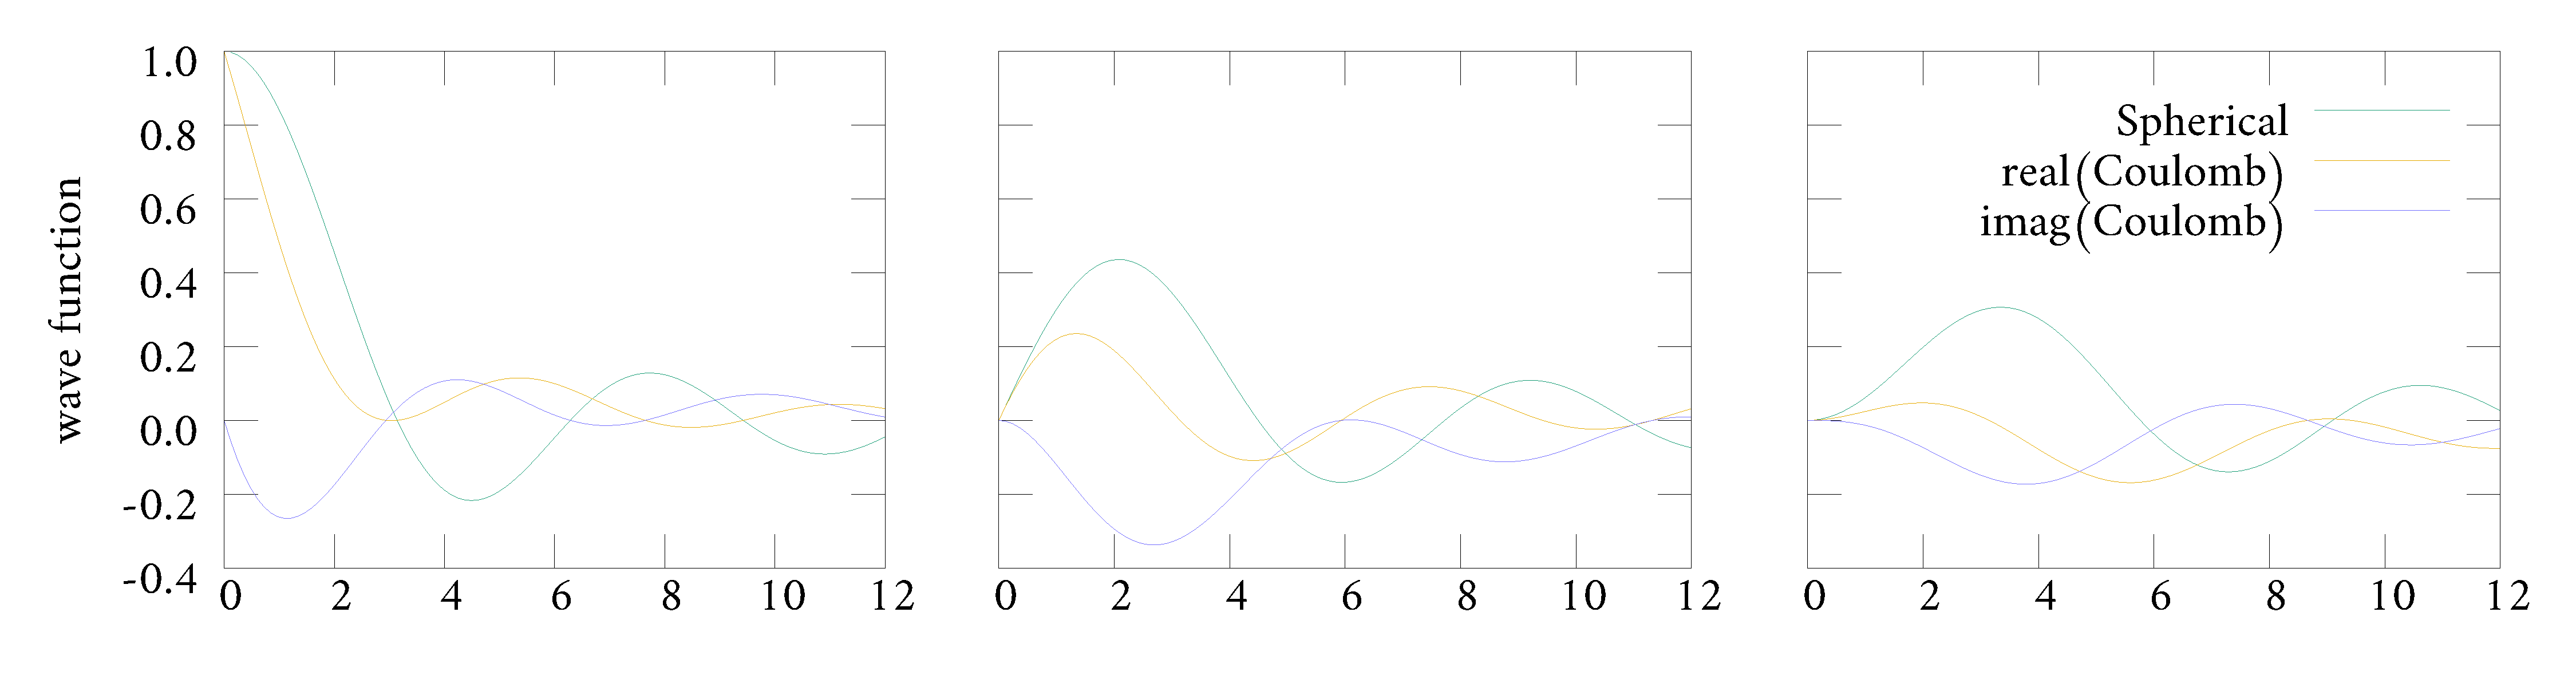
\includegraphics[width=\textwidth]{Figures/RBF/RadialPart}
\caption{Radial part of spherical waves and Coulomb waves (confluent hypergeometric function approximated with 35 terms each) for $l=0$ (left), $l=1$ (centre) and $l=2$ (right).
The Coulomb waves are not normalised.}
\label{fig:RadFun}
\end{figure}

A third expansion that is availible \textit{e.g.} in the program \prog{ezDyson} \cite{ezDyson} is an asymptotic Coulomb wave expression for vanishing momentum in which the confluent hypergeometric function can be approximated by a Bessel function as
\begin{equation}
\lim_{k\rightarrow 0} F_1(l+1+\frac{i}{k}, 2l+2, 2ikr) =(2l+1)! (2r)^{-l-\frac 12} J_{2l+1}(\sqrt{8r})
\end{equation}
where $Z=-1$ is assumed and $J_{2l+2}(x)$ is the Bessel function that is connected to the spherical Bessel functions $j_l(x)$ via the relation $j_l(x)=\sqrt{\frac{\pi}{2x}} J_{l+\frac 12}(x)$ \cite{Lifschitz}.
This case is separately available in \prog{ezDyson} \cite{ezDyson}.

The spherical Harmonics \cite{SphHarm} moreover have the form
\begin{equation}\label{eq:SphHarm}
Y_l^m(\theta,\phi)= (-1)^{(m+|m|)/2} i^l \sqrt{\frac{2l+1}{4\pi}\frac{(l-|m|)!}{(l+|m|)!}}  P_l^{|m|}(\cos(\theta)) e^{im\phi}
\end{equation}
where $P_l^m(x)$ are associated Legendre polynomials \cite{Lifschitz}.
The spherical harmonics are orthonormalised according to
\begin{equation}
\int Y_l^{\dagger m}(\phi,\theta)  Y_{l'}^{m'}(\phi,\theta) d\vec{r}=\delta_{l,l'} \delta_{m,m'}
\end{equation}
and have the property
\begin{equation} \label{eq:dipoleRule}
\int Y_l^{\dagger m}(\phi,\theta) \vec{r} Y_{l'}^{m'}(\phi,\theta) d\vec{r}=\delta_{l,l'\pm 1} C_{l,l', m,m'}
\end{equation}
if not both $l$ and $l'$ are $0$ where $C_{l,l',m,m'}$ are Clebsch-Gordan coefficients.
The relation  (\ref{eq:dipoleRule}) governs the dipole transition probabilities of molecular systems.

Both expansions (\ref{eq:spherWave}) and (\ref{eq:CoulWave}) do not take the molecular potential into account but give an easy picture for the photoelectron.
Since the spherical wave basis is obtained under the assumption of no potential $V(\vec{r})$, this is is assumed to be a good approximation for photodetachement when the initial state is neutral whereas the Coulomb wave expansion takes into account the electrostatic potential of the remaining anion at larger distances to the molecule and thus is more reasonable for ionised remainder systems \cite{do_modCoul}.
Due to these obvious deficiencies of the inflexible expansions, some modifications are used by several authors which involve the coise of an effective charge $Z^*<1$ in the expansion (\ref{eq:CoulWave}) \cite{do_modCoul} and an orthogonalisation of the expansion with respect to the DO \cite{do_modCoul,do_orthonorm,do_orthonorm1,do_pworth}.
The latter can be shown to be equivalent to a respective shift of the expansion centre such that the expectation value of the dipole moment of the DO vanishes \cite{do_orthonorm}.

In this work the spherical waves (\ref{eq:spherWave}) are used as reference basis for the computed solutions for an easier interpretation and comparison of different results.
To do so, the numerically obtained solution $|\Psi_\text{n}\rangle$ is projected onto spherical waves for different $l$ and $m$ which will be referred to as partial wave coefficient.
%j_l\left(kr\right), Y_l^m\left(\theta, \phi\right) Y^{\dagger,m}_l\left(\theta_k, \phi_k\right) 

In addition to the previously discussed questions abuot the relation of analytic and numeric FEFs, the infinite degeneracy of the analytical solutions has no numerical counterpart and thus leads to problems which are discussed on the example of the ionisation of a hydrogen-like atom whose analytical FEF is of the form (\ref{eq:CoulWave}) but with arbitrary coefficients for each term whose only prerequisite is that their squares add up to one \cite{Lifschitz}.
%
%In addition to the transition from a continuous to a discontinuous spectrum, also degerarcy plays an important role.
%This can be best discussed when taking the example of the ionisation process of a hydrogen atom where the corresponding FEF has the analytic form

The Coulomb wave basis is, given its energy $E=\frac 12 |\vec{k}|^2$, infinitely degenerate in the direction of $\vec{k}$ as well as in the quantum numbers $l$ and $m$.
%Hence the wave function of a photoelectron can consist of any superposition of the form (\ref{eq:CoulWave}), chosing the coffecients $c_{l,m}$ accordingly.
However, the coefficients of the physically observable FEF are determined by the matrix elements of the dipole operator with the DO (\ref{eq:sigma_do}).  
Considering the ionisation of hydrogen in its ground state, the FEF is in one of the three $p$-waves because the probability to access any of the other vaccum-states with the correct energy vanishes due to dipole selection rules eq. (\ref{eq:dipoleRule}) for spherically symmetric systems.

Unfortunately, as shown in section \ref{ch:resBench}, the considerations made above are not true for the numerical solution anymore where a finite set of superpositions is obtaind which, due to numerical treatment, differ in energy and thus can not be assigned to a common value of $\vec{k}$.
Chosing the energetically best-fitting solution though might in principle result in a function with vanishing contribution of the $p$-type orbitals whereas, for a slightly changed computational schem or target energy it could yield a solution with large $p-$contributions and high intensity, respectively.

%The coefficients $c_{l,m}$ moreover are arbitrary coefficients to this end since any of the linear combinations solves the SE for a given kinetic energy.
%Hence analytical the solutions are not only continuous in $\vec{k}$, but also infinitely degenerate in $l$ and $m$.
%In contrast to this, the numerical solution will be a linear combination of some of these terms; in the easiest case it is close to one of these $l$ and $m$.
%However, for the case of ionisation from the hydrogen ground state only the contributions with $l=1$ will lead to a transition probability; having a solution of $l=2$-character would lead to vanishing probability.
%Hence, the lifting of degeneracy would lead to intensities that are very sensitive to the kinetic energy of the photoelectron since the $l=1$ solution might be only few meV off that solution of $l=2$-type.
%Moreover, the numerical grid may influence this dependency since it could, by accident, supporting certain symmetries.
%
%A detailed discussion of the conceptual complications arising from this is not found in the literature.
%The FEF used to describe the ionisation of H$_2$ as discussed in \cite{H2pDeCleva} is chosen as that function which fits the target energy best.
%However, in their formulation this energy is well-separated from the others % (spline base without boundary conditions, leading to non-hermitian Hamiltonian). -> do they implicitly use some boundary conditions ?
%They also discuss formulation as minimisation problem: More stable but they don't need it.
%which will be later shown to be not the case here.

\subsection{Stieltjes Imaging}
\label{ch:stieltjes}
The Stieltjes imaging \cite{stieltjesCeder,langhoff3,stieltjeLanczos,langhoff} provides an elegant way to use the numerially obtained FEFs of a discrete character lying above the ionisation threshold for PES calculations.% by using moment theory.
To correct on the different character of the spectrum and the smaller extend of the numerically obtained solution, the Stieltjes imaging approach uses spectral moments 
\begin{equation} \label{eq:SpecMom}
\mu_n=\int_0^\infty \epsilon^n df(\epsilon)
\end{equation}
where $n<0$ denotes the order of the moment, $\epsilon=E-E_0$ is the transition energy and 
\begin{equation}
\frac{df}{d\varepsilon}=\frac 23 (E-E_0) \left|\langle \Psi_0 |\vec{\hat{d}}|\Psi_f \rangle \right|^2
\end{equation}
is the oscillator strength with the dipole operator $\vec{\hat{d}}$, the energes $E_0$ and $E$ of the ground state $|\Psi_0\rangle$ and final state $|\Psi_f\rangle$, respectively.
Since the final state can be of bound state character $|\Psi_\alpha\rangle$, where the enegies are discrete, as well as of continuous character $|\Psi_\varepsilon\rangle$ with continuous spectrum, one can rewrite the spectral moment (\ref{eq:SpecMom}) as \cite{langhoff3} 
%Inserting the closure relation $\sum_\alpha |\Psi_\alpha\rangle\langle \Psi_\alpha|+\int |\Psi_\varepsilon\rangle\langle \Psi_\varepsilon| d\varepsilon$ for the full (anatlytic) Hamiltonian results in
\begin{align}\label{eq:M_n_ana}
   \mu_n&=
   %\sum_\alpha \langle \Psi_0 |\hat{d} (\hat{H}-E_0)^n|\Psi_\alpha\rangle\langle \Psi_\alpha| \hat{d} | \Psi_0  \rangle
      %+ \int  \langle \Psi_0|\hat{d} (\hat{H}-E_0)^n|\Psi_\varepsilon\rangle\langle \Psi_\varepsilon| \hat{d} | \Psi_0  \rangle d\varepsilon \\
      \sum_\alpha \left(E_\alpha-E_0\right)^n \left|\langle \Psi_0 | \hat{d}| \Psi_\alpha\rangle \right|^2 + 
         \int_{0}^\infty \varepsilon^n \left|\langle \Psi_0 | \hat{d}| \Psi_\varepsilon\rangle \right|^2 d \varepsilon
\end{align}
where $\varepsilon$ denotes the kinetic energy of the FEF.
%However, inserting the unity expression for the numerical Hamiltonian which does not have continuum functions but an everywhere discrete spectrum and hence $L^2$-integrable eigenfunctions results in
Since, in contrast to the analytic case (\ref{eq:M_n_ana}), the numeric Hamiltonian has a discrete spectrum, the respective spectral moments here are of the form
\begin{equation} \label{eq:M_n_num}
      \mu_n= \sum_{j=0}^N (E_j-E_0) \left| \langle \Psi_0 | \hat{d}| \Psi_j\rangle \right|^2
\end{equation}
where $N$ denotes the number of eigenfunctions $|\Psi_j\rangle$ and the sum accounts for the bound as well as unbound states \cite{stieltjeLanczos,stieltjesCeder}.
%For a good numerical approximation, the expressions (\ref{eq:M_n_num}) and (\ref{eq:M_n_ana}) should be similar for as many $n$ as possible where, due to convergence of the spectral moments, $n<2$ \cite{stieltjesCeder}.
%These considerations are used in the Stieltjes imaging approach with moment theory \cite{langhoff, langhoff2}.
Assuming that the first $2l-1$ spectral moments can be restored by the numerical Hamiltonian in good approximation, they can be used to obtain a histogram representation of the cross section of the form
%In the protocol derived from this scheme thus the oscillator strength $|\langle \Psi_0|\hat{d}|\Psi_\text{el}\rangle|^2$ is approximated by the histogram
\begin{equation}
\sigma(\varepsilon)=\frac 23 \frac{df}{d\varepsilon}
      =\frac 23 \begin{cases} 0 & 0< \varepsilon <\varepsilon_1(l) \\
      \frac 12 \frac{(f_i+f_{i+1})}{\varepsilon_{i+1}-\varepsilon_i}  & \varepsilon_j(n)<\varepsilon<\varepsilon_{j+1}(l)\\
      0   & \varepsilon_n(l)<\varepsilon \end{cases}
\end{equation}
%where $f_i$ is obtained from enforcing the relation (\ref{eq:M_n_num}) for $n=1,\hdots, m$ which is done by solving the matrix equation
where $(\varepsilon_i,f_i)_{i=1,...,l}$ are a principal pseudo spectrum \cite{stieltjeLanczos}. 
The values $\varepsilon_i$ and $f_i$ are obtained from an eigenvalue equation of a symmetric tridiagonal matrix whose diagonal elements $\alpha_i$ and off-diagonal elements $\beta_i$ can be found as parameters a function 
\begin{equation}\label{eq:I_z1}
I(z)=\frac{\beta_0^2}{z-\alpha_1-\frac{\beta_1^2}{z-\alpha_2-\hdots-\frac{\beta_{l-1}^2}{z-a_l}}}
\end{equation}
which contains the full information about the first $2l-1$ spectral moments and has the alternative form \cite{nesbet}
\begin{equation} \label{eq:I_z2}
I(z)=\frac{\mu_0}{z}+\frac{\mu_1}{z^2}+\hdots+\frac{\mu_{2l-1}}{z^{2l}}
\end{equation}
where $\mu_i$ are the spectral moments (\ref{eq:m_n_num}) \cite{nesbet}.
The key task in Stieltjes imaging is the transformation from the form (\ref{eq:I_z2}) to (\ref{eq:I_z1}) \cite{nesbet}.

In practice, the Stieltjes imaging is very demanding if energetically narrow transitions occur since many terms in expression (\ref{eq:M_n_num}) are needed for convergence, making this method efficient mainly for low energy range \cite{H2pDeCleva}.
%Another disadvantage that no asymtotic information about this scheme is reported \cite{H2pDeCleva}.

\section{Finite Differences and Finite Volumes}
\label{ch:FD}
The most common and straightforward approach to solve differential equations such as the SE numerically is via the so-called finite difference (FD) scheme.
Starting from the one-particle SE in atomic units
\begin{equation} 
\left(-\frac 12 \nabla^2 + V(\vec{r}) \right) \Psi(\vec{r})=E\Psi(\vec{r})
\end{equation}
where $V(\vec{r})$ is an arbitrary potential at this point.
Considering a general problem where the low symmetry does not support a product ansatz as \textit{e.g.} eq. (\ref{eq:radSE}) which reduces the dimensionality and thus the complexity of the problem, the kinetic energy operator has in a matrix representation at least $6$ off-diagonal terms per line whose non-banded structure requires iterative solvers \cite{fd_Cart}.
An important disadvantage of finite difference schemes is that they require the evaluation points to be on a regular grid whose stepsize is governed by the sharpest features in the system while local refinement is hardly available.
If considering molecules and thus Coulomb-shaped potentials $V(\vec{r})$, the finest structures are expected to be close to the nuclei whereas at larger distances a respectively dense grid is not needed and thus computations of FEFs with a reasonable box size become very expensive \cite{richardsFD}.
Nonetheless, there are applications of this scheme to the SE \cite{fd_Cart,fd_Cart2}, some of them with massive parallelisation using MPI and multiple GPUs \cite{fd_gpu}.

To overcome this bottleneck for systems with non-uniform parameters, often the finite volume method is used.
The finite volume method is an integral method that is not based on a regular grid.
Instead, for the estimation of the kinetic energy Gau\ss's theorem $\int_V \nabla \vec{u}(\vec{r}) dV=\int_{S} \vec{u}(\vec{r}) \vec{n}dS $ is used where $\vec{u}(\vec{r})$ is a vector-valued function and $\vec{n}$ is the normal vector on the surface $S$ of the volume $V$ under consideration.
Chosing $\vec{u}(\vec{r})=\nabla\Psi(\vec{r})$ yields the relation
\begin{equation} \label{eq:kinFV}
   \nabla^2\Psi(\vec{r})=\lim_{V\rightarrow 0} \frac{ \int_{\partial V} \nabla\Psi(\vec{r}) \vec{n} dS}{V}.
\end{equation}
This scheme becomes especially interesting when the finite volume elements are chosen to be Voronoi cells \cite{Son_Chu0}.
A Voronoi-tesselation is associated with a grid and is constructed such that the Voronoi cell $T_i$ consists of all points in space that are closer to the point $i$ than to any other points in the grid, see Figure {\ref{fig:VorCell} \cite{voronoi,voronoi1,voronoi2}.

This description has the advantage that the quantities on the right-hand side of (\ref{eq:kinFV}) can be associated with properties of the Voronoi-Cell, leading to the first-order approximation of the kinetic energy
\begin{wrapfigure}{l}{0.5\textwidth}
   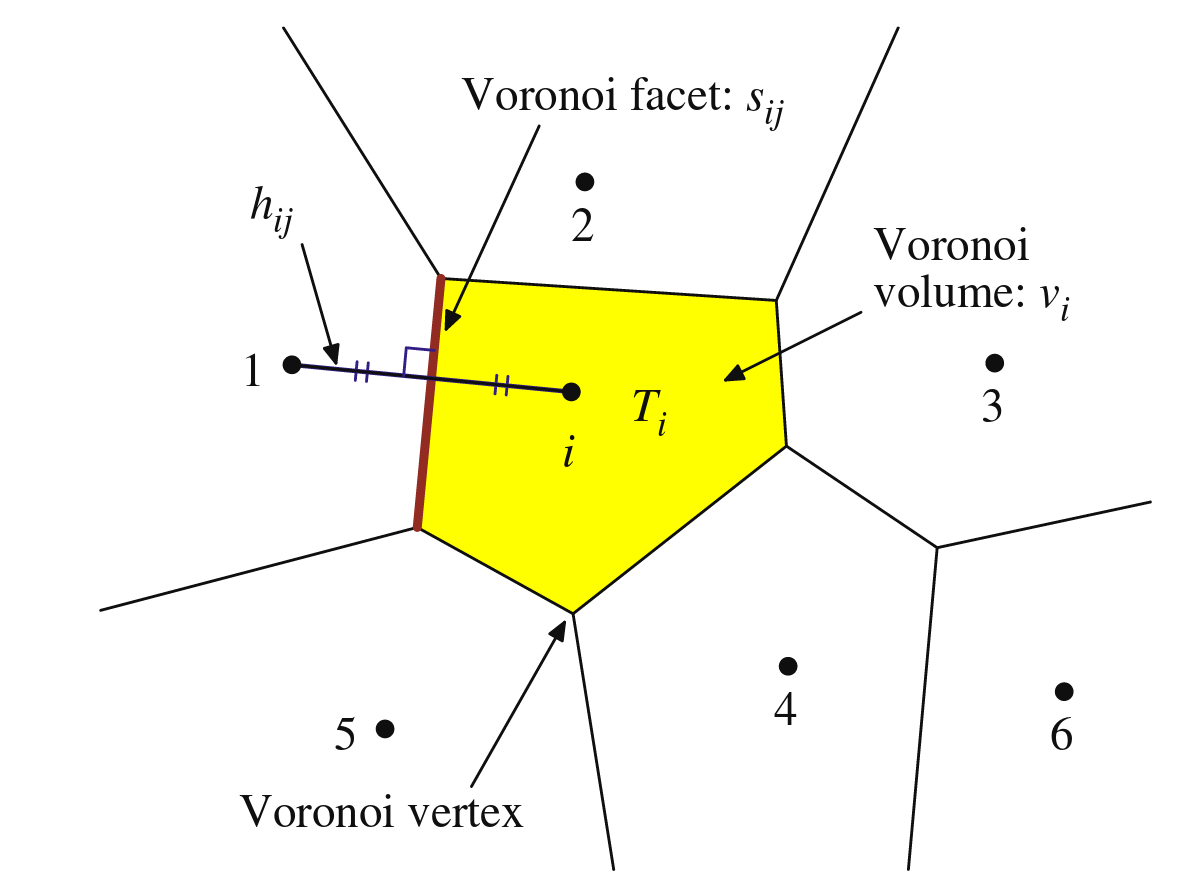
\includegraphics[width=0.5\textwidth]{Figures/VoronoiFD}
   \caption{2-dimensional Voronoi diagram on an arbitrary distribution of seven points \cite{Son_Chu}.}
   \label{fig:VorCell}
\end{wrapfigure}
\begin{equation}\label{eq:kinVoron}
   \nabla^2\Phi(\vec{r}_i)=\frac{1}{v_i} \sum_j^\text{neighbours} \frac{\Psi(\vec{r}_j)-\Psi(\vec{r}_i)}{h_{ij}} s_{ij}a
\end{equation}
where $v_i$ is the volume of the $i$-th Voronoi-cell (yellow area in Figure \ref{fig:VorCell}), $h_{ij}=|\vec{r}_i-\vec{r}_j|$ is the distance between the centres of the $i$-th and $j$-th Voronoi-cells (bolt black line) and $s_{ij}$ is the area of the common facet of the $i$-th and $j$-th Voronoi cells (red line in Figure \ref{fig:VorCell}).

Such a scheme is applied, \textit{e.g.}, by Son and Chu \cite{Son_Chu0, Son_Chu} to the time-dependent SE, studying multi-photon ionisation of several molecular systems.

%\section{Discrete Variable Representation and Splines}
\section{Pseudospectral Methods}
\label{ch:dvr}
Under the term (pse)udospectral methods a large group of methods is comprised which treat the differential equation of interest variationally using an orthogonal basis $\{\varphi_i(\vec{r})\}$, hence seeking for a solution of the form
\begin{equation}
\Psi(\vec{r})=\sum_i^n c_i \varphi_i(\vec{r})
\end{equation}
where $c_i$ are coefficients to be found \cite{SpectMeth}.
In the pseudospectral methods the basis functions $\varphi_i(\vec{r})$ are smooth global functions, \textit{e.g.} $\varphi_{\vec{k}}(\vec{r})=e^{\text{i}\vec{k}\vec{r}}$, resulting in the Fourier space \cite{Fourier}.
Alternatively Jacobi, Chebychef or Legendre polynomials are commonly used \cite{PSbook}.

To find the corresponding coefficients, the problem is solved on a grid, leading to a linear system of equations.
Depending on the technique used for determining the coefficients, it can be seen as a high-order FD or high-order FEM.
One prominent advantage of this class of methods is that the error of the solution $\psi(\vec{r})$ usually decays exponentially with the number $n$ of basis functions and the grid can be chosen coarsely, making the numerical scheme very efficient \cite{PSbook, Tannor}.
In addition, many formulations allow for an implementation making use of the fast fourier transform \cite{PSbook}.

A special representative subgroup of the pseudospectral methods are the so-called discrete variable representation (DVR) schemes which are frequently used to study electronic structure and vibrational problems in molecules \cite{yipDVR,impLDVR,coulDVR}.
Since this scheme is applicable in one dimension only, often symmetry-adapted coordinates such as spherical coordinates are used product functions such as (\ref{eq:RadSE}) are applied.

The basis functions used in this scheme commonly are Lagrange polynomials \cite{taoDVR,impLDVR,coulDVR} whose nodes are chosen by a general Gau\ss\, quadrature rule \cite{impLDVR} or from a quadrature rule for the radial Coulomb function which is in particular popular whene electronic structure problems are considered \cite{coulDVR,Tannor}.
Even if the DVR provides a flexible and fast-convergent basis, an extension to higher dimensionality can only be achieved by a product ansatz and thus is applicable to problems with high symmetry.

Moreover, as for the other pseudospectral methods, the system matrices are dense and thus the solution is numerically expensive.
This is at least partially solved by using a hybrid scheme of the finite element and DVR scheme where the DVR scheme is used on small segment only, connected by single bridge-functions each \cite{taoDVR,impLDVR}.

\section{Radial Basis Functions}
The radial basis function (RBF) technique is based on an arbitrary point distribution with very general properties.
The ansatz functions $\varphi_i(\vec{r})$ used in this technique need to be spherically symmetric, \textit{i.e.} $\varphi_i(\vec{r})=\varphi_i(|\vec{r}|)$ and are placed at the grid points on a given domain.
The RBF-scheme is used not only for solving differential equations but is also a usefull tool for interpolation of scattered data in arbitrary dimensions \cite{rbfInterpol} and surface reconstruction from scattered data \cite{rbfSurf}.

Among the commonly used functions are, besides linear and cubic ones, multiquadratic ($\sqrt { r^2 + r_0^2 }$), inverse multiquadratic ($( r^2 + r_0^2)^{-\frac 12}$) and Gaussian ($ \exp(-\frac{r^2}{2r_0^2})$) functions are to be mentioned where $r_0$ is the radius, respectively \cite{rbfSE,rbfWave}.

If the parameter $r_0$ is chosen reasonably, the scheme is numerically stable and fast convergeing \cite{rbfSE}, but the choise of $r_0$ can be non-trivial especially for highly non-regular grids where a good quality of of the representation between two points with a large distance require a respectively large radius $r_0$ whereas too large radii can make the scheme numerically instable for close-lying points.
Moreover the resulting system matrices are dense due to the global definition of the ansatz functions, making it compputationally expensive when large domains are considered.
%Another advantage is the straight-forward implementation and generality of this method.
%\begin{wrapfigure}{r}{0.6\textwidth}
%   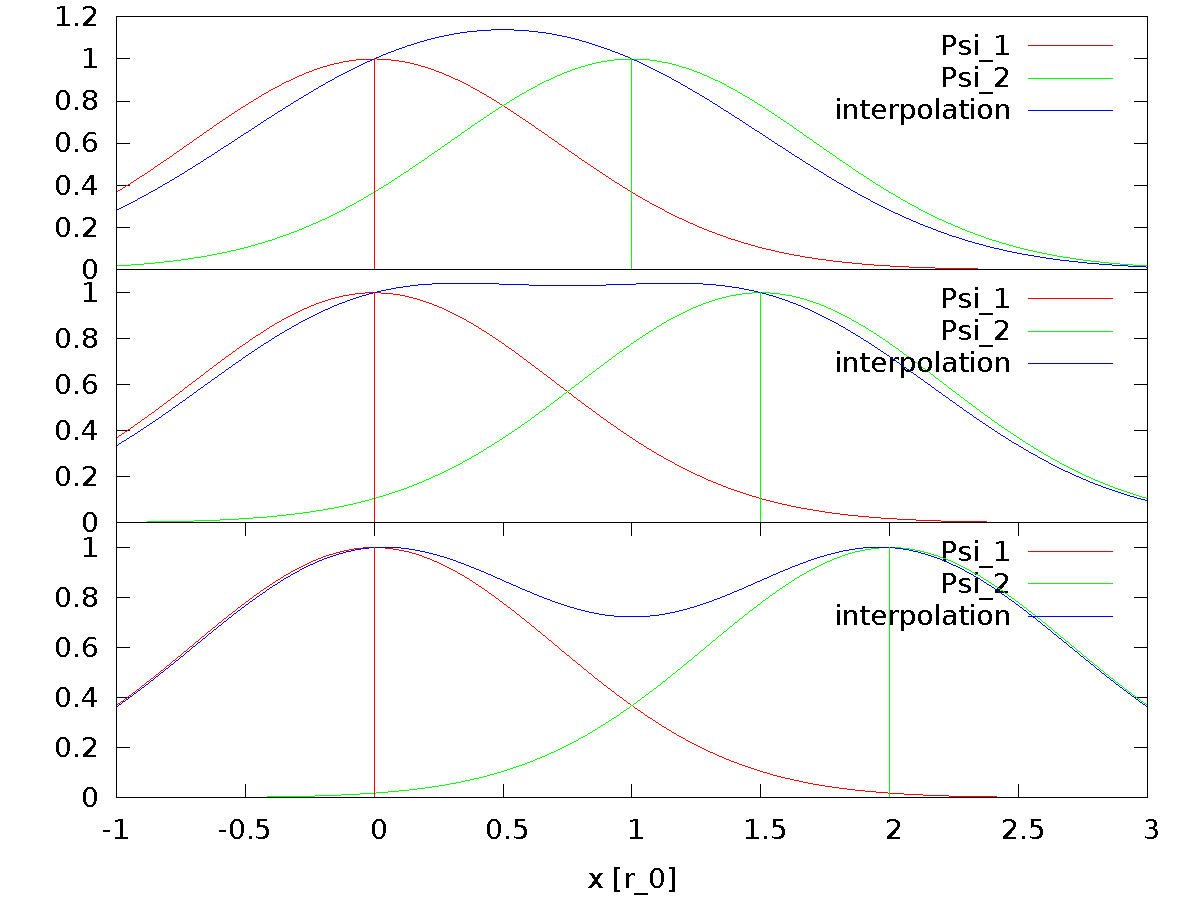
\includegraphics[width=0.6\textwidth]{Figures/RBF/RBFerror}
%   \caption{A function (blue) represented in a RBF basis with Gaussian functions, centred at different distances compared to the broadening parameter $r_0$.}
%   \label{fig:rbfError}
%\end{wrapfigure}
%An important disadvantage of the RBF scheme is that the space between two interpolation points is interpolated non-linearly and, depending on the distance of the two functions, the values are over- or underestimated.
%This error is visualised in Figure \ref{fig:rbfError} for the case of a function that is one at both supporting points, represented by a Gaussian RBF basis.
%The intermediate values of the function depends strongly on the ratio of the broadening $r_0$ and the difference between the supporting points.
%While this behaviour is not problematic for visual purposes, it may introduce a substructure which can lead to unintended behaviour of the solution.

\section{Finite Elements}
\label{ch:introFEM}
In the FEM the differential equations to be solved are formulated in their weak form which is an integro-differential equation and can be understood as a generalisation of the differential equation \cite{femBraess}.
Starting with the well-known (strong) form of the SE defined on a domain $ \Gamma$ in atomic units which are used here and in the following chapters
\begin{equation} \label{eq:SEstrong}
-\frac 12 \nabla^2\Psi(\vec{r})+ V(\vec{r})\Psi(\vec{r})=E \Psi(\vec{r}) \qquad  \vec{r}\in \Gamma
\end{equation}
with the condition 
\begin{equation}
    %\lim_{\vec{r}\longrightarrow \infty} \Psi(\vec{r})=0
    \Psi(\vec{r})=0  \qquad \vec{r} \in \partial \Gamma
\end{equation}
for the boundary domain $\partial \Gamma$ which is assumed to be Lipschitz continuous.
The first term in equation (\ref{eq:SEstrong}) corresponds to the kinetic energy and $V(\vec{r})$ is a potential that is not further specified at this point.
The unknowns of this equation are the wave function $\Psi(\vec{r})$ and respective energy $E$.
To bring equation (\ref{eq:SEstrong}) into the weak form, it is first multiplied by the complex conjugate of a test function $\Phi(\vec{r})$ which fulfils the same boundary conditions and needs to be differentiable.
In the second step, one integrates over the whole space of interest resulting in the equation
\begin{align}
\int d \vec{r} & \left( - \frac 12 \left(\nabla^2\Phi^*(\vec{r})\right)\Psi(\vec{r})
               + V(r) \Phi^*(\vec{r}) \Psi(\vec{r})\right) = E \int d \vec{r} \Phi^*(\vec{r}) \Psi(\vec{r}).
\end{align}
The kinetic energy term can be symmetrised using Green's first identity $\int_\Gamma (\nabla^2\Psi)\Phi^* d\vec{r}=\int_{\partial \Gamma} (\nabla\Psi)\Phi^* ds -\int_\Gamma (\nabla\Psi)(\nabla\Phi^*) d\vec{r}$ to obtain the final expression
\begin{align}\label{eq:SEweak}
\int_\Gamma d \vec{r} & \left(  \frac 12 \left(\nabla\Phi^*(\vec{r})\right) \left(\nabla\Psi(\vec{r})\right) 
               + V(r) \Phi^*(\vec{r}) \Psi(\vec{r})\right) = E \int_\Gamma d \vec{r} \Phi^*(\vec{r}) \Psi(\vec{r})\\
   % &\lim_{\vec{r}\longrightarrow \infty} \Phi(\vec{r})=0.\qquad
   % \lim_{\vec{r}\longrightarrow \infty} \Psi(\vec{r})=0.
    &\Phi(\vec{r})=0\quad
     \Psi(\vec{r})=0\quad  \vec{r}\in\partial\Gamma
\end{align}
which is denoted as the weak form of the SE.
A function $\Psi(\vec{r})$ is considered as a solution of (\ref{eq:SEweak}) if the equation holds for any test function $\Phi(\vec{r})$.
Since usually only real-valued bases functions are used, in the literature the complex conjugation is omitted.
Moreover, from a mathematical point of view, since $\Phi(\vec{r})$ is an arbitrary function, complex conjugation does not change anything here but it will be shown later that it is more reasonable from a physical point of view if the weak formulation is defined as given in equation (\ref{eq:SEweak}).

The weak formulation (\ref{eq:SEweak}) has two main changes in its properties compared to the strong formulation (\ref{eq:SEstrong}).
The first is that any solution of (\ref{eq:SEstrong}) solves (\ref{eq:SEweak}) while the space of solutions of the weak form is larger since only first derivatives need to be defined, which lead to the terms weak and strong respectively.
In addition, a weak solution is defined only up to a cardinal number of zero; hence changing the values of a given solution $\Psi(\vec{r})$ along a finite number of planes in three dimensions yields a function that still solves (\ref{eq:SEweak}).
These properties play an important role here since they allow \textit{e.g.} the use of piecewise linear basis functions as they are commonly used in the FEM scheme which do not have a second derivative and whose first derivative is undefined on certain planes.

As usual for numerical methods, in the FEM scheme one restricts the search for solutions to a subspace spanned by a finite set of test functions for both $\Psi(\vec{r})$ and $\Phi(\vec{r})$, leading to the Petrov-Galerkin scheme.
To get best flexibility for the wave function, the domain $\Gamma$ is subdivided into finite volume elements with a close packing.
These volume elements, denoted as finite elements, give this method its name.
Having this subdivision of space, the ansatz (basis) functions $\varphi(\vec{r})$ used to construct $\Psi(\vec{r})$ and $\Phi(\vec{r})$ are defined as piecewise polynomials being non-zero only on one or few elements.\\
Considering $\Gamma$ to describe a 2D-plane, the elements can be, for example, triangles as shown in Figure \ref{fig:2Del}.
Enumerating the vertices of the triangles as $\vec{r}_i\, i=1,\hdots ,N $, the piecewise linear (Langrange-) basis functions are defined as
\begin{equation}\label{eq:femAnsatz}
   \varphi_i(\vec{r}_j)=
           \begin{cases} 1  & j=i \\
                         0  & j\neq i \end{cases}
\end{equation}
resulting it two-dimensional ``hat'' functions as depicted in Figure \ref{fig:2Del} for an index $i$.
\begin{wrapfigure}{r}{0.75\textwidth}
   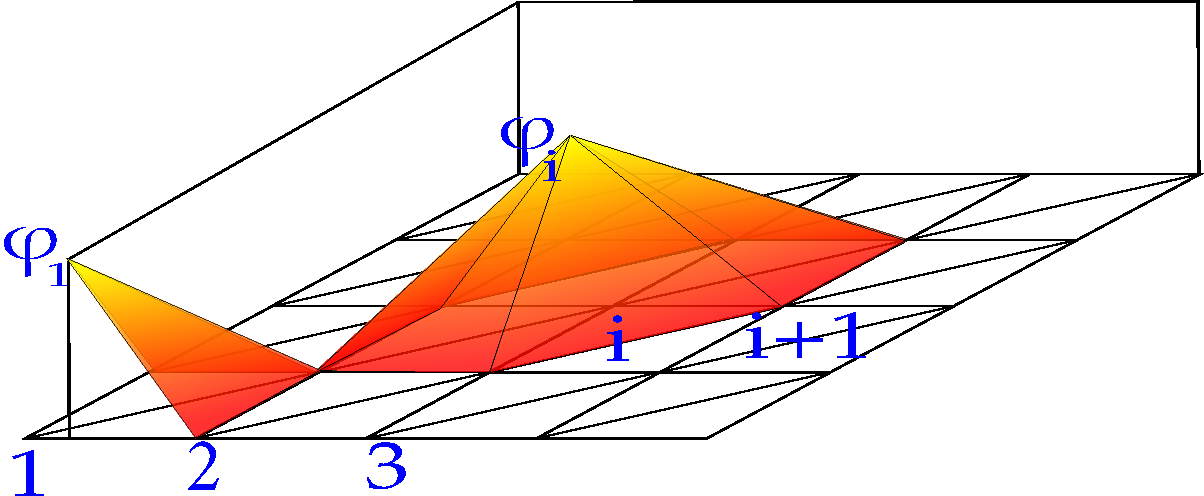
\includegraphics[width=.75\textwidth]{Figures/FEM2d-crop}
   \caption{Example of finite elements in 2D of triangular shape and linear basis functions $\varphi_i(\vec{r})$ defined on them.}
   \label{fig:2Del}
\end{wrapfigure}
This definition of a basis ensures continuity of the solution over $\Gamma$ while the first derivatives are continuous only within each element.
To assure continuity of the first derivatives as well, second order polynomials are needed.
At the boarder of $\Gamma$, respectively truncated ``hat'' functions are used whose coefficients are given by the boundary condition.

As usual in variational schemes, the wave function of interest is constructed as a linear combination of these basis functions $\Psi(\vec{r})=\sum_i c_i \varphi_i(\vec{r})$ where $c_i$ are weighting coefficients.
The test functions are chosen from the same space of ansatz functions, testing each basis separately $\Phi(\vec{r})=\varphi_j(\vec{r}), j\in {1,\hdots, N}$.
Hence, the SE (\ref{eq:SEweak}) with the finite basis reads
\begin{multline}
     \sum_i \int d  \vec{r} \left(\frac 12 \left(\nabla\varphi_i(\vec{r})\right) \left(\nabla\varphi_j(\vec{r})\right) +
                             V(r) \varphi_i(\vec{r}) \varphi_j(\vec{r}) \right) c_i =
               E \sum_i \int d \vec{r} \varphi_i(\vec{r}) \varphi_j(\vec{r}) c_i \\
                      \quad \forall j \in \{1,\hdots ,N\}
\end{multline}
which is the $j$-th component of the generalised matrix eigenvalue problem
\begin{equation}\label{eq:SEmat}
\left(\frac 12 \mat{A} +\mat{V}\right)\vec{c} =E\mat{M}\vec{c}. 
\end{equation}
\text{with}
\begin{align} \label{eq:FEMmatrix}
      \mat{A}_{ij} &=\int d \vec{r} \left(\nabla\varphi_i(\vec{r})\right) \left(\nabla\varphi_j(\vec{r})\right) \quad
      \mat{V}_{i,j}&=\int d \vec{r} V(\vec{r}) \varphi_i(\vec{r}) \varphi_j(\vec{r}) \quad
      \mat{M}_{i,j}&=\int d \vec{r} \varphi_i(\vec{r}) \varphi_j(\vec{r})
\end{align}
and the vector $\vec{c}$ in equation (\ref{eq:SEmat}) contains the coefficients $c_i$ to be found.

The quality of this basis depends strongly on the size and shape of the finite elements:
The stronger the solution varies, the smaller element sizes or higher order ansatz functions are required to be able to represent the wave function.
Knowledge about ranges of sharp structures and areas with smooth variation of the wave function $\Psi(\vec{r})$ hence is crucial for the setup of a good mesh.

In chapter \ref{ch:fem} more details about the finite element formulation are given with a special focus on how to setup a grid that is well suited for describing free particles in quantum mechanics.

\section{Hybrid Methods}
In addition to the three methods presented above also mixed forms exists, utilizing the advantages of the respective ideas.
One of the most prominent combinations of the above-mentioned methods is the finite element discrete-variable representation (FE-DVR) \cite{impLDVR,taoDVR}.
In this schem, a DVR is used with a set of ansatz functions each defined on a given interval only, referred to as the finite element.
A single function connects these intervals respectively, similarly to the ``hat'' functions in FEM.
Using this approach, more flexibility is obtained by varying the size of the elements or the number of basis functions per element which is especially advantageous for problems involving a Coulomb potential where the local kinetic energy varies strongly \cite{yipDVR}.
Moreover, the usually dense matrix of DVR schemes changes to a block-structure, each weakly coupled \cite{taoDVR}.

Another scheme based on the FEM scheme are the so-called spectral elements \cite{sem1,sem2,sem3} used by several authors on quantum mechanical problems.
In contrast to the FE-DVR-scheme it is based on the weak formulation and typically uses Chebychev or Lagrange polynomials \cite{sem1} and hence allows for larger elements than usual FEM.
While the spectral elements are found to be well suited for linear problems, they require a complex implementation and lead to denser system matrices.
The larger density in the resulting matrices in general leads to a reduced numerical stability and computationally more expensive solution strategies.
Finally, complex geometries usually benefit more from smaller elements that from higher orders \cite{hf_dreyer}.

A successfull variety of spectral elements and the finite element method is the so-called spectral difference method \cite{SpectDiff,sd_mult}.
In this scheme, a spacially uniform grid is used (as usual in the finite difference scheme) while employing a stepwise defined pseudospectral basis.
The appealing properties of this method are an exponential convergence as known from finite difference methods by employing the sparsity of the equation system obtained in FEM \cite{SpectDiff}.

More advanced methods based on the spectral difference schemes are available as well \cite{sd_mult,sd_unstructured} but are for brevity not discussed here in more detail.

\section{Wavelets}
\label{ch:wavelet}
The wavelet method was developed in the 1980s \cite{waveletLA} and combines the advantages of the Fourier method and FEM by decomposing objects into features of different scales but using a local basis \cite{waveletLA, dahlke, FdFeWavelet}.
Even though wavelets posess very advantagous features, they are not very well-established untill today.
The most prominent and widely distributed application of Wavelets is compression of data as used for example in the jpeg2000 standard \cite{iso15444}.

%A wavelet is a basis of the function space $L_p(\mathbb{R}^d)$ of functions $\phi(\vec{r})$ for which $\int \phi(\vec{r})^p d\vec{r}<\infty$ which has the form
In general, a wavelet is a basis of the function space $L_p(\mathbb{R}^d)$ \textit{i.e.}, the space of functions $\phi(\vec{r})$ for which $\int \phi(\vec{r})^p d\vec{r}<\infty$ where $\vec{r}\in\mathbb{R}^d$.
A particular wavelet is defined by a finite set of orthonormal mother wavelets $\varphi_i(\vec{r})$ for which
\begin{equation} \label{eq:waveBasis}
\varphi_{i,j,\vec{\alpha}}(\vec{r})=m^{\frac{j}{2}} \varphi_i(\mat{M}^j\vec{r}-\vec{\alpha})
\end{equation}
with the expanding scaling matrix $\mat{M}$ (\textit{i.e.} all eigen values have modulus larger than one), $m=|det(\mat{M})|$ and the running indices $j\in \mathbb{Z}\, \vec{\alpha}\in \mathbb{Z}^d$ span $L_p(\mathbb{R}^d)$ \cite{dahlke}.
%The condition for (\ref{eq:waveBasis}) to be a wavelet basis is that these functionst span $L_p(\mathbb{R}^d)$.
In practice, this very general definition is often restricted by additional requirements such as orthogonality of $\varphi_{i,j,\vec{\alpha}}(\vec{r})$ and only one mother-wavelet $\varphi(\vec{r})=\varphi_i(\vec{r})$ is used.
For brevity, in the following only the space $L_2(\mathbb{R})$ with $\mat{M}=2$ is considered which corresponds to the initial definition of wavelets \cite{Tasche}.
The most prominent representatives are the Haar-wavelet and Daubechies wavelets which are orthogonal functions with finite support as depicted in Figure \ref{fig:wavelets}.
%The most prominent and by far simplest example of a wavelet is the so-called Haar-wavelet wich hase one mother wavelet of the form
%\begin{equation} \label{eq:haar}
%\varphi(x)=\begin{cases} 1 &0\leq x < \frac 12 \\ -1 & \frac 12 \leq x <1 \\ 0 & \text{else}\end{cases}
%\end{equation}
%for which (\ref{eq:waveBasis}) is a orthonormal basis with compact support.

Another set of orthogonal wavelets with compact support are the Daubechies wavelets that are a series with increasing smoothness and support.
The Haar-wavelet, shown in Figure \ref{fig:wavelets} on the left, can be seen as the first order Daubechies-wavelet.
In contrast to most other bases, here no smootheness properties are required but are helpfull of course since the functions to be represented usually are smooth \cite{daubechies}.
\begin{figure}
   \begin{subfigure}{0.32\textwidth}
   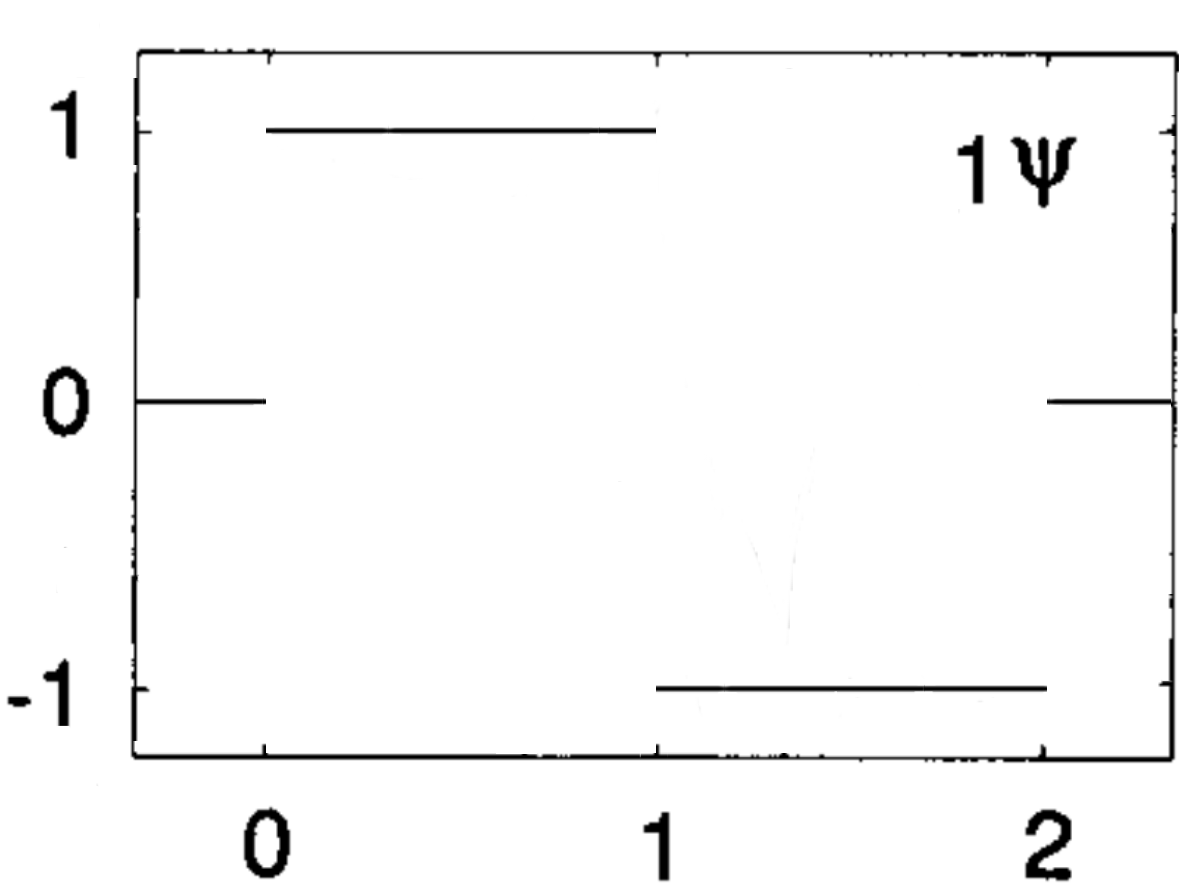
\includegraphics[width=\textwidth]{Figures/Daubechies1}
   \end{subfigure}
   \begin{subfigure}{0.32\textwidth}
   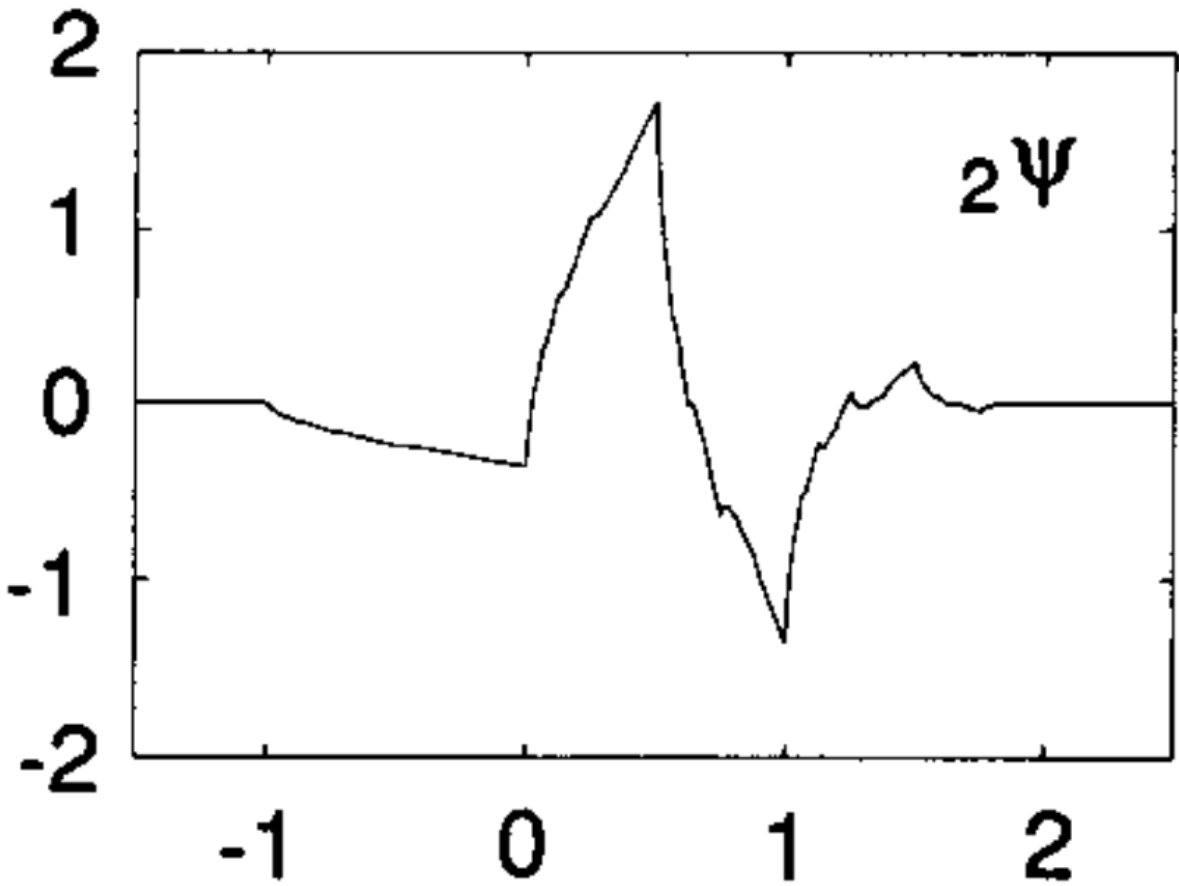
\includegraphics[width=\textwidth]{Figures/Daubechies2}
   \end{subfigure}
   \begin{subfigure}{0.32\textwidth}
   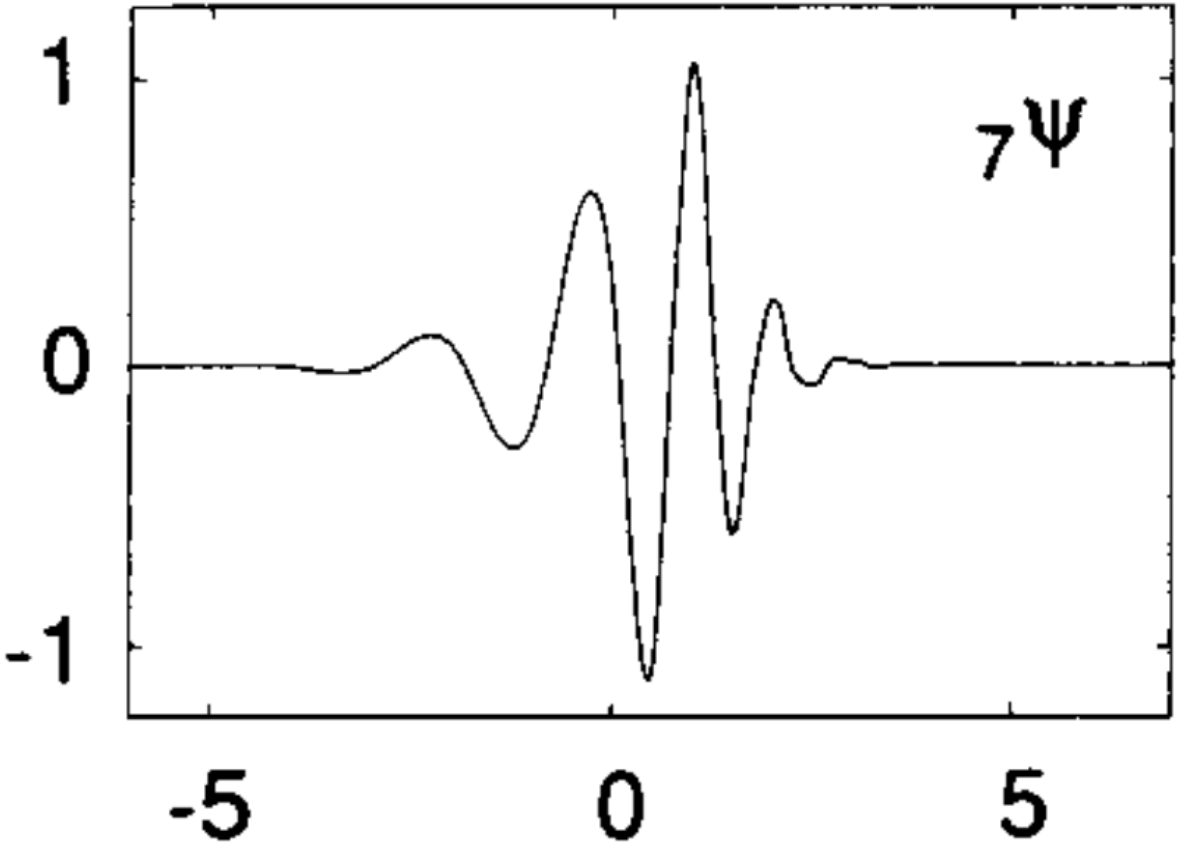
\includegraphics[width=\textwidth]{Figures/Daubechies7}
   \end{subfigure}
   \caption{Daubechies wavelets of the orders 1, 2 and 7 (from left to right) \cite{daubechies}.}
   \label{fig:wavelets}
\end{figure}

Besides their broad use in data compression and analysis, wavelet bases also provide a handy tool to solve partial differential equations and are found to have similar numerical properties as the FEM \cite{FdFeWavelet,CoulWavelet}.
When applying a wavelet basis to solve a partial differential equation, the weak form (\ref{eq:SEweak}) is used, leading to a similar description as in the FEM scheme \cite{dahlke}.
However, not all wavelets provide a valid basis for partial derivatives since, for example, the Haar-wavelet has a constant derivative of zero and the Daubechies-wavelet $2$ (shown in Figure \ref{fig:wavelets}) is only semi-differentiable at some points \cite{WaveletChem}.
At the same time hand the generality of the wavelet formulation allows to use problem-specific bases that are \textit{e.g.} especially adapted to certain pseudo-differential operators, increasing the convergence properties \cite{dahlke}.
Finding such optimised bases in a systematic way is under current research but one can expect that they could obtain numerically stable, fast and accurate partial derivative solvers \cite{dahlke,kunoth}.


\chapter{Finite Element Methods}
\label{ch:fem}
As a conclusion of the previous chapter one can see that the number of methods that are currently available to describe a free electron function in presence of an intricate electrostatic background potential is not that large.
In this work the method of choise to model the free electron function is the FEM which had been applied to quantum mechanical problems already by several authors \cite{fem_hydro, vib_fem, fe_hf, fe_dft1}, however, to the best of my knowledge, only to bound state problems so far.
A brief review about these works is given in section \ref{ch:feQM}.
Besides its large flexibility and computational efficiency pointed out in section \ref{ch:introFEM} already, the large amount of available libraries for FEM \cite{libmesh,dealII,freefem, hermes,oofem} is another advantage of practical importance due to the complexity of the generation of a suitable mesh, assembling of matrices and solution of matrix equations.

In the following chapter the integration of the matrix elements (section \ref{ch:feInt}) and set up of the mesh (section \ref{ch:feAss}) will be described.
Thereby the focus is put on the application to the one-particle SE that is to be solved with molecular ESP.
Since the interest thereby is on free particle solutions, the spectrum is expected to be very dense and the wave function to be delocalised, requirering for well-designed boundary conditions.
A discussion of various boundary conditions and asymptotic descriptions available for FEM is described in section \ref{ch:BC}.

\section{Finite Element Calculations in Quantum Chemistry}
\label{ch:feQM}
The FEM is mainly known from engineering disciplines where it is used in a broad range of applications such as modelling of fluids \cite{fluid1,fluid2}, heat transfer and flow \cite{heat1, heat2,heat3} or material deformation under mechanical stress \cite{deform1, deform2}.
However, also several different quantum chemical problems have been solved with this method: SE solvers for small systems such as light atoms \cite{fem_hydro,fem_He,fem_He1, fem_h1, LiGS_fem} or diatomics \cite{fem_H_refine}, vibrational model systems \cite{vib_fem} and solid state problems \cite{fem_crystal, fem_crystal1}.
Moreover, even Hartree-Fock \cite{fe_hf} and DFT calculations on systems up to the size of benzene \cite{fe_dft1, fe_dft2, fe_dft3} have been performed, yielding results comparable to those obtained by the usual linear combination of atomic orbitals (LCAO) approach.

The above-mentioned publications have shown that the FEM is able to obtain reasonable results for molecular systems where the errors were comparable to those obtained with standard quantum-chemistry schemes even though their computational costs are higher.
This suggests that the FEM is a good tool for computations in the field of quantum chemistry for going beyond the capabilities of the established schemes such as the description of unbound states.

%\section{From Weak Form to a Matrix Equation}
\section{Integration of Matrix Elements and Formulations of the Equation System}
\label{ch:feInt}
In section \ref{ch:introFEM} the basics of the FEM were described and the generalised eigen system shown in eq. (\ref{eq:SEmat}) to solve the SE was derived.
Here this is taken as starting point and a closer look at the computation of the matrix elements as well as solving strategies for the large sparse generalised eigen problems are taken.

The generalised eigenproblem as given in eq. (\ref{eq:SEmat}) consists of three matrices.
Since the ansatz functions (shape functions) $\varphi_i(\vec{r})$ have only a small support, most of the matrix elements are zero. 
However, in two and three dimensions no distinct band structure is achievable and the matrices are irreducible.
Thereby matrix elements are zero when the elements involved are not neighboured.
The computation of the non-zero matrix elements involve an integration as \textit{e.g.} the overlap integral $\mat{M}_{i,j}=\int d \vec{r} \varphi_i(\vec{r}) \varphi_j(\vec{r})$ of ansatz functions,.
Since these functions are the same for all elements, the evaluation of these integrals can be done via a lookup-table or an efficient numerical integration scheme whose required order is well-known and need only be multiplied by the Jacobian of the respective elements involved.
The matrix elements $\mat{A}_{i,j}=\int d \vec{r} \left(\nabla \varphi_i(\vec{r})\right)\left(\nabla \varphi_j(\vec{r})\right)$ consist similar to those of $\mat{M}$ of overlap integrals of known functions.
The only matrix containing system-specific information is the potential $\mat{V}_{i,j}=\int d \vec{r} \varphi_i(\vec{r}) V(\vec{r}) \varphi_j(\vec{r})$ which requires numerical integration by which $V(\vec{r})$ is approximated as a spline of given order.

After assembling the matrices the eigenpair $(e_i, \vec{c}_i)$ of the system
\begin{equation} \label{eq:SEmat2}
\left(\frac 12 \mat{A}+\mat{V}\right)\vec{c}_i = e_i \mat{M}\vec{c}_i
\end{equation}
need to be found where $e_i$ should be closest to the analytic value of the kinetic energy of the photoelectron.
Since matrix eigenvalue equations with several thousands of dimensions occur in many fields, numerous schemes have been developed to solve them efficiently \cite{davidson,arnoldi, gpusolver,krylov}, a selection of them is described in section \ref{ch:ghep}.
Despite the numerical complexity due to the high dimensionality of this problem (several thousands of basis functions) the second problem is due to the fact that the eigenenergies $e_i$ are expected to be close to each other since the corresponding analytical problem has a continuous spectrum in this range.
It is well known in numerics that this leads to instabilities especially for the eigen vectors, making a regularisation of the problem (described in section \ref{ch:regular}) indispensable.

\section{Element Types and Mesh Types}
\label{ch:feAss}
Among the FEM formulations several `flavours' were designed for different purposes.
Given a certain equation to be solved in FEM there are in general two systematic ways to increase the accuracy.
The first way is to increase the number of elements witch is referred to as the $h$-FEM approach \cite{dreyer,}.
The refinement of the mesh is in principle always possible but technically demanding since it is not known in which regions of a mesh are too coarse in general \cite{dreyer}.
To overcome this, some FEM implementations such as that of \prog{Libmesh} \cite{libmesh} which is used here, provide an adaptive mesh refinement scheme, iteratively refining the mesh using local error estimations and thus fully automatic \cite{libmesh}.
But theses schemes are numerically demanding and hence can be only applied to benchmark systems.

The second strategy is called $p$-FEM. 
In the $p$-FEM scheme, the order $p$ of the test functions in increased, resulting in smother and more flexible solutions.
This scheme requires a large set of functions to be implemented but is known to yield good results if the function is smooth \cite{p-fem}.
While standard FEM-libraries usually have only $p=1,2$ implemented, others have high-order polynomials implemented \cite{hermes}.
Combined schemes where the grid-size as well as the element order are adapted is referred to as $hp$-fem \cite{hp-fem}.

Besides these different refinement strategies, finite element types also vary in their use of the degrees of freedom.
While Lagrange elements are integrated by evaluating certain inner or boarder points, \textit{e.g.} in Argyris or Hsieh-Clough-Tocher elements also first or even second derivatives are evaluated \cite{femPraxis,femCiarlet}.
Moreover, the arrangement of elements one distinguishes conforming and the more general non-conforming meshes \cite{nonconfFEM}. In case of the latter, more general structures are supported as \textit{e.g.} hanging nodes which occur when a vertex of one element is on the edge of an other as can be found in Figure \ref{fig:HexBenz} \cite{femCiarlet}.
The setup of the mesh is, as mentioned above already, critical to the quality of the solution and hence of special importance.
Moreover, it is technically non trivial to set up a close packing of volume elements with the desired properties in a systematic way.
There are different element types available, each with their techniques for set up.
Although in principle any element shape can be chosen, in three dimensions only tetrahedral (simplex), prism- and pyramid-shaped as well as hexahedral elements commonly are used.
By choosing the element shape and the polynomial order, also the type of shape functions is defined.
%When using hexahedral elements the ansatz functions usually are of the type $\varphi(\vec{r})=x^ky^lz^m$ where $p=k+l+m$ is the element order.

When considering meshes to describe molecular properties it is clear that the element size should be smaller in the vicinity of the nuclei while it may be broader at larger distances.
One way to create a hexahedral mesh with local refinement is to start with a coarse uniform lattice and subdivide the hexahedra where necessary as shown in Figure \ref{fig:HexBenz} for a benzene molecule.
Another way is to setup small regular cubic grids around the nuclei and expand them radially in boxes of growing size as shown in Figure \ref{fig:HexDia}.
These brick-shaped elements however have the disadvantages that the regular cube-like structures therein might be not well-suited for atoms and molecules that rely rather on spherical shapes.
%Further hexahedral elements are known to give less accurate solutions than tetrahedra which are commonly used nowadays \textcolor{green}{cite}.

%\begin{wrapfigure}{r}{\textwidth}
%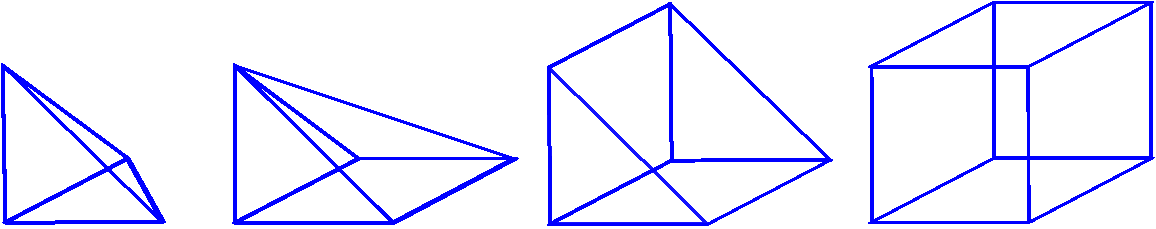
\includegraphics[width=\textwidth]{Figures/Elements3d-crop.pdf}
%\caption{The different Shapes of 3D elements.}
%\end{wrapfigure}
Another approach used by Lehtovaara \textit{et al.} \cite{fe_dft2} is to put layers of polyhedra around the atoms with increasing number of points and radii.
Thereby the overlapping regions of these spheres are removed by deleting elements that are closer to another atom.
\begin{figure}
  \begin{subfigure}{0.23\textwidth}
   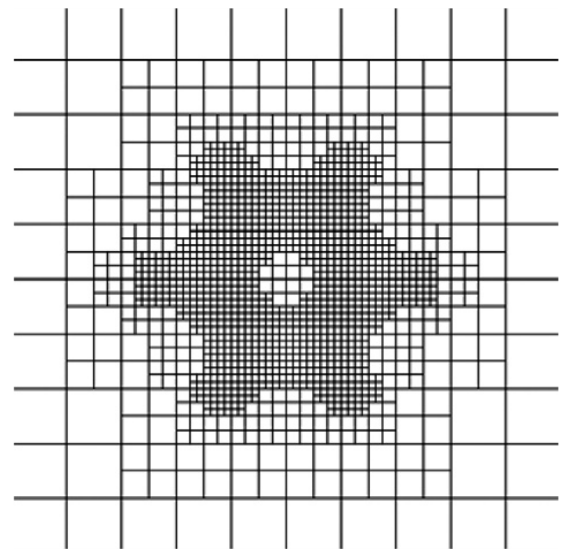
\includegraphics[width=\textwidth]{Figures/QuadMeshBenzene}
   \vspace{-43mm}\caption{$\qquad\qquad\qquad\qquad$}
   \label{fig:HexBenz}
  \end{subfigure}
  \begin{subfigure}{0.28\textwidth}
   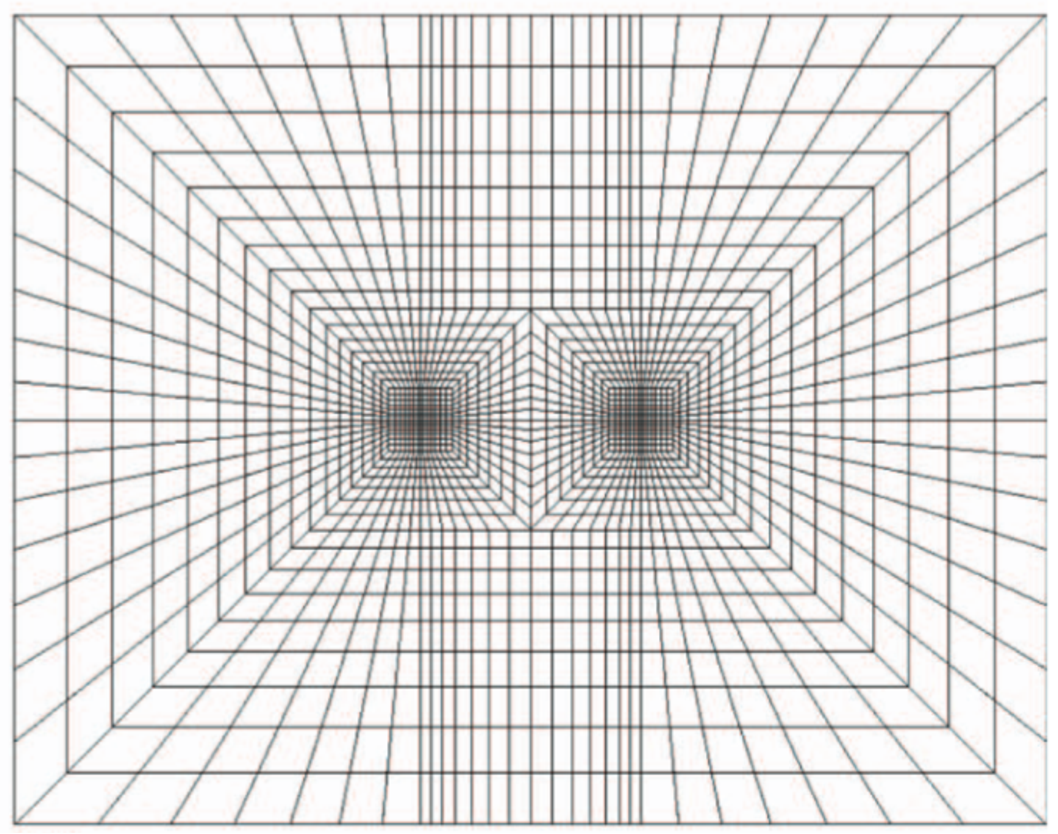
\includegraphics[width=\textwidth]{Figures/QuadDiatomic}
   \vspace{-43mm}\caption{$\qquad\qquad\qquad\qquad\quad$}
   \label{fig:HexDia}
  \end{subfigure}
  \begin{subfigure}{0.23\textwidth}
   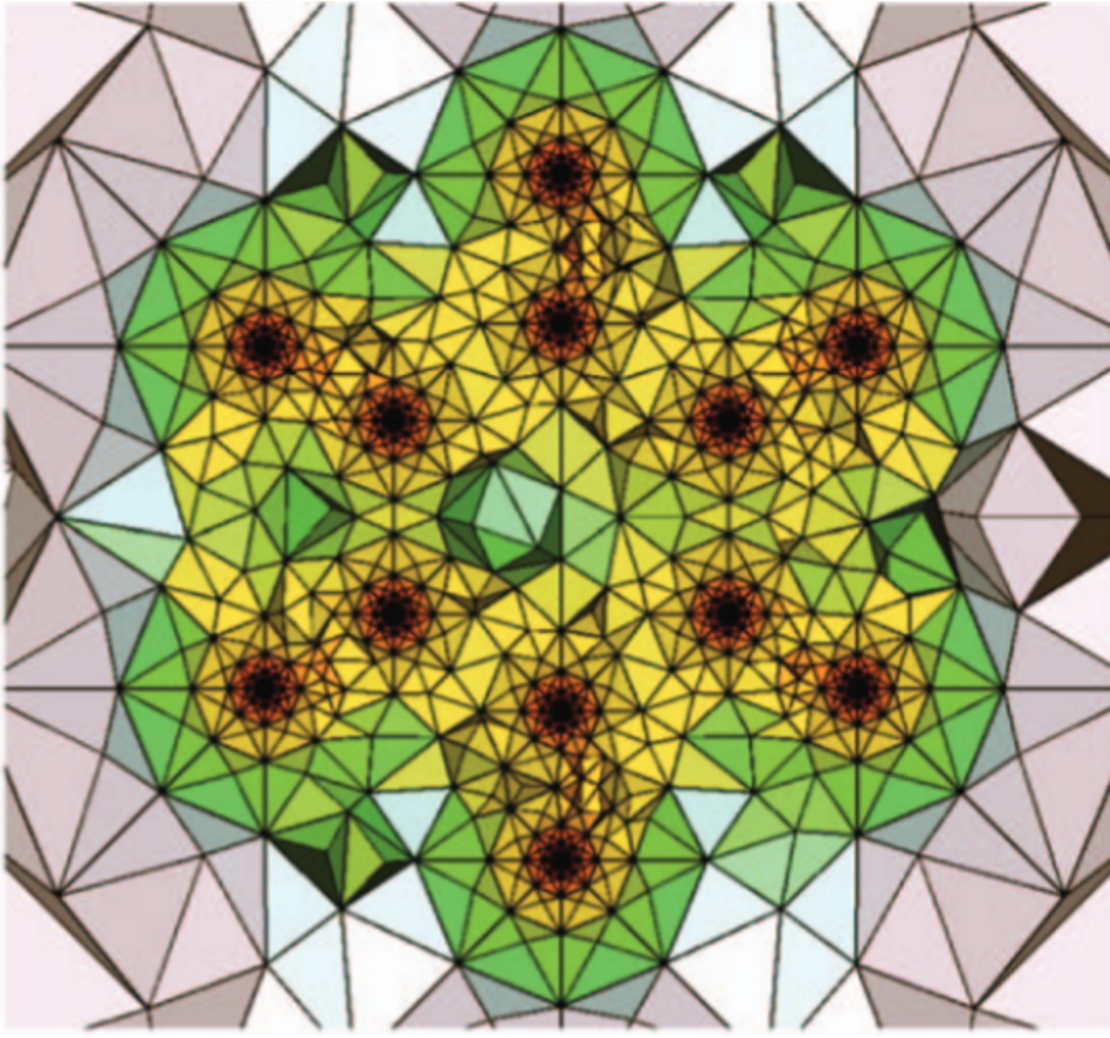
\includegraphics[width=\textwidth]{Figures/PolyBenzene}
   \vspace{-42mm}\caption{$\quad\qquad\qquad\qquad\quad$}
   \label{fig:PolyBenz}
  \end{subfigure}
  \begin{subfigure}{0.23\textwidth}
   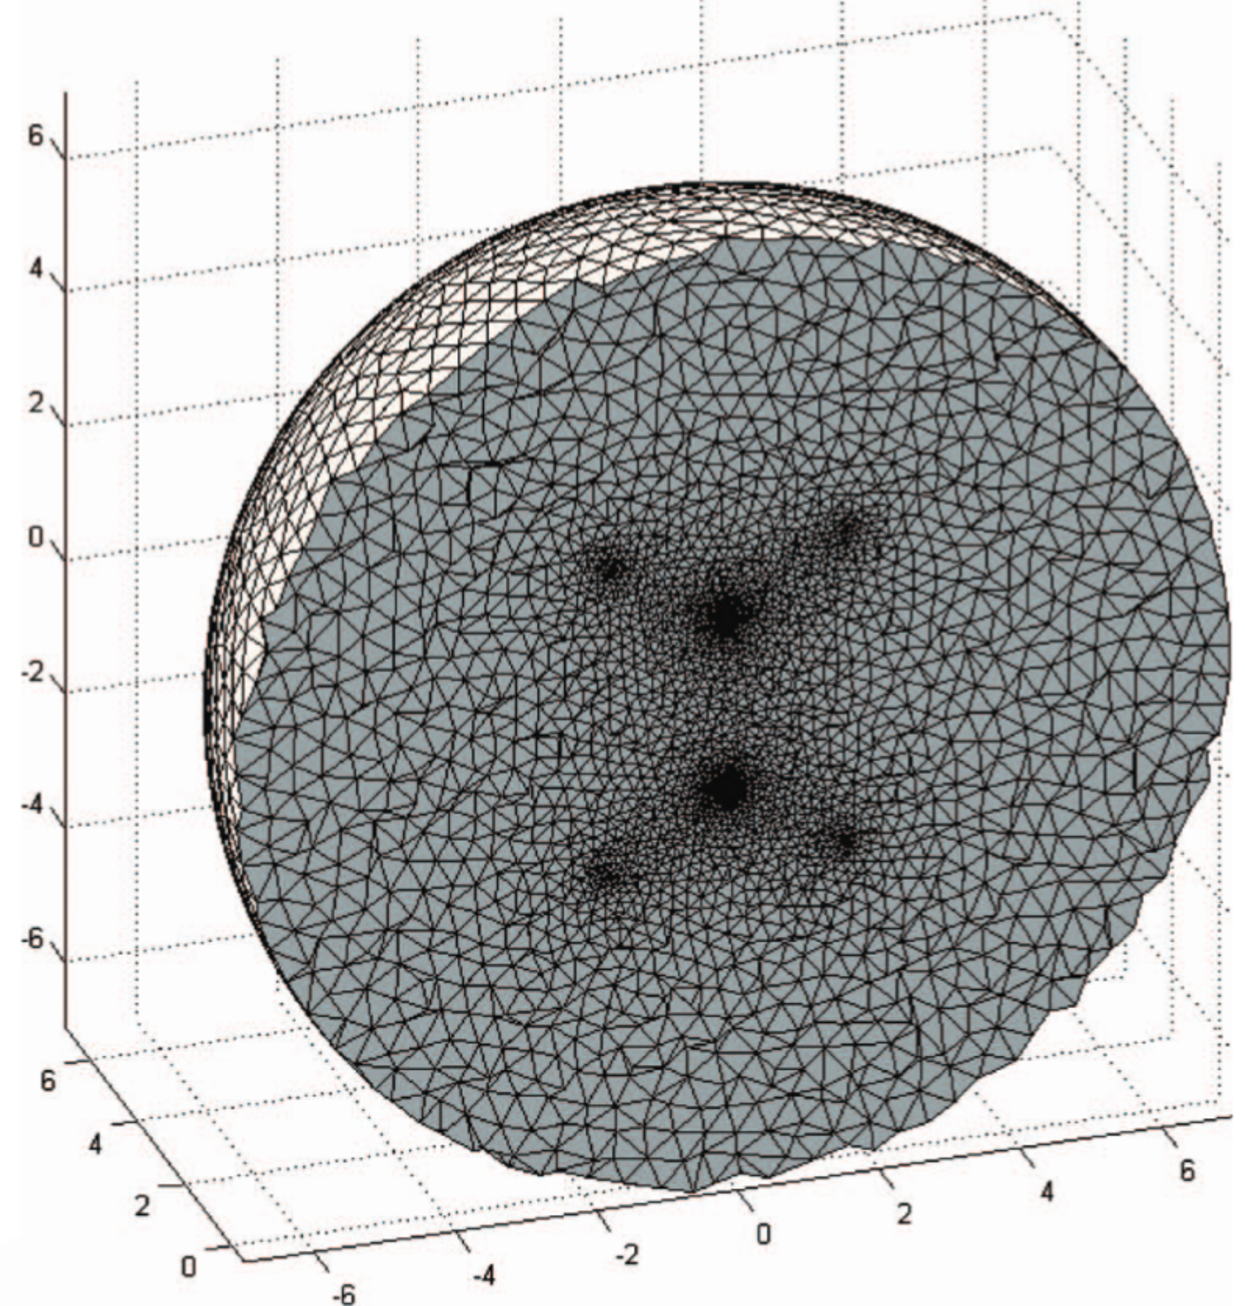
\includegraphics[width=\textwidth]{Figures/AdaptiveEthylene}
   \vspace{-44mm}\caption{$\qquad\quad\qquad\qquad$}
   \label{fig:AdapEthyl}
  \end{subfigure}
  \vspace{34mm}
  \caption{2D cuts through 3D meshes for molecular systems obtained with different schemes for local refinement:
    (a) hexahedral elements adapted for the benzene molecules \cite{fe_dft1}
    (b) hexahedral mesh for a diatomic \cite{fe_hf}
    (c) Polyhedral mesh for a benzene geometry \cite{fe_dft2}
    (d) Adaptive refined tetrahedral Mesh for ethylene. \cite{fe_hf}
    }
\end{figure}
The mesh obtained with this procedure for a benzene molecule \cite{fe_dft1} is shown in Figure \ref{fig:PolyBenz}.

When restricting oneself to tetrahedral elements, other design principles are possible: Since they are simplexes in three dimensions, they can be designed from general grids using \textit{e.g.} Voronoi \cite{voronoi} or Delaunay \cite{delaunay} tessellations (the latter is described in section \ref{app:delaunay} in appendix) from a set of points with the required properties.
Son and Chu \cite{Son_Chu, Son_Chu0} constructed sets of points resembling molecular geometries by inserting $N$ spherical grids with different radii $r_i$ around the atoms and cutting off the overlapping regions.
Thereby the respective radii are chosen as
\begin{equation}
r_i=\frac{il}{N-i+\frac{lN}{r_\text{max}}} \qquad i=1,\hdots ,N 
\end{equation}
where$r_\text{max}$ is the radius of the largest sphere and $l$ is a parameter smoothly changing between a linear $l\rightarrow \infty$ and a $1/r$-mapping.
As spherical grids they suggested the use of Lebedev-grids \cite{lebedev} and a design of Womersley \cite{Womersley2001,Sloan}.
A more detailed discussion about the choices of grids will be given in section \ref{sec:grid}.
%Choises for angular and radial grid distributions in this scheme are discussed in.% the chapters \ref{app:Sphere} and \ref{app:radius} respectively.

A more entangled method is used by Alizadegan \textit{et al.} \cite{fe_hf}. 
They start with an initial guess for the wave function and create a grid whose distances are inverse proportional to the second gradient of the electron density
\[
d \propto \left[ max\left\{\left|\frac{\partial^2 \rho}{\partial^2 x}\right| ,
                           \left|\frac{\partial^2 \rho}{\partial^2 y}\right| ,
                           \left|\frac{\partial^2 \rho}{\partial^2 z}\right| \right\} \right]^{-1}.
\]
which gives an estimate for the error due to linear approximation within each element.
After solving the eigenvalue equation on this grid, they recompute another mesh on the basis of the new function, iterating this procedure several times.
A cut through a mesh obtained by this procedure is shown in Figure \ref{fig:AdapEthyl}.

\section{Boundary Conditions}
\label{ch:BC}
Boundary conditions have not been addressed in this thesis so far for any of the methods but play an important role for the properties of the solution.
Hence there is a large number of boundary conditions.
The simplest case applicable here are Dirichlet-boundaries, requiring the wave function to vanish at the boundaries of the finite element box.
In the FEM this condition can be applied especially simple by setting the coefficients of the outermost shape functions to zero.

Due to the large extend of the free particle, these boundaries however are unphysical if they are not applied at distances that are several times larger than the wavelength.
However, considering a particle with $0.1\,$eV kinetic energy, its wavelength is $~4.4\,$Angstroms and the box would need to have a diameter of several tens of Angstroms which is not feasible any more while kinetic energies in the $m$eV-range would lead to even worse scenarios.

%These considerations make clear that a more advanced boundary condition is needed which has only local influence on the wave function.
%In the following sub chapters, three boundaries that can be applied in FEMs are introduced and discussed.
Besides the numerical restriction to a finite box also mapping schemes can be used as \textit{e.g.} $x=\tan (\frac y2)$ that maps $[-\infty:\infty]$ to $[-\pi:\pi]$ \cite{PSbook}.
However, using such a mapping directly is infeasible since the oscillations of the wave function would become arbitrarily sharp in the mapped range and hence the representation of the FEF would still be poor.

\subsection{Complex Absorbing Potential}
\label{ch:cap}
The complex absorbing potential (CAP) is a method often found in the literature when describing particles with infinite extent\cite{bauch1, bauch2}.
In this scheme, an artificial potential usually of the form
\begin{equation}
   W_\text{CAP}(\vec{r})=\begin{cases} i\nu(\vec{r}-\vec{r}_0)^2 & \vec{r}>\vec{r}_0 \\
                                           0    & \text{else} \end{cases}
\end{equation}
is added where $\vec{r}_0$ is larger than the bound part of the system.
Such a potential damps the reflection of the wave function at the boarders and thus enhances the quality of states obtained on a finite region \cite{cap1, cap2}.
However, studies with different shapes of these potentials show that it influences the wave function not only close to the boarders and a proper design of the parameters is non-trivial \cite{CAPfreshlook}.

To minimise the error due to the CAP, the parameter $\eta$ can be chosen such that its dependency on the energy vanishes in first order, \textit{i,e.} $\eta\frac{dE}{d\eta}=0$ \cite{CAPccEOM,CAPfreshlook}.
Moreover, due to non-hermiticity the usual scalar product is not suitable when calculating overlap integrals any more.
Too strong $\eta$ introcudes reflections, too weak $\eta$ lead to unstable resonances, making them strongly basis-set dependent \cite{CAPfreshlook}.
Moreover, for Helmholtz problems, a dependence of the error on the frequency was observed \cite{babuska}.

The idea of damping down a function and making sure no reflections are scattered back to the region of interest is common to further approaches as \textit{e.g.} absorbing boundary conditions \cite{Engquist}, transparent boundaries \cite{HelmhPrec}, perfectly matched layer schemes \cite{pmlBook,pml1, pml2} or certain variable transformations \cite{taoDVR}.

\subsection{Mode-matching Schemes}
Consider the solution in an inner and outer region as different variables following the equations
\begin{equation}
   \nabla^2\Psi_1 +V(\vec{r})\Psi_1-E\Psi_1=0 \qquad \nabla^2\Psi_2 -E\Psi_2=0 
\end{equation}
whereby the outer function needs to satisfy the Sommerfeld condition $r^\alpha \left(\frac{\partial \Psi_2}{\partial r} - ik \Psi_2  \right)\rightarrow 0$.
These equations are coupled by the conditions
\begin{equation}
\Psi_1=\Psi_2  \qquad \nabla \Psi_1 \vec{n}=\Psi_2 \vec{n}
\end{equation}
to ensure continuity of the solution and the gradient normal to the boundary \cite{AstleyMM}.
Thereby, the asymptotic behaviour of the outer function is ensured by taking basis functions that individually fulfil the condition and the boundaries enter the weak formulation since the application of Greens' theorem leads to an extra term.

The mode-matching scheme can be considered as a generalisation of the R-matrix approach in a finite element formulation.

\subsection{The Boundary Element Method}
The boundary element method (BEM) can be used as a self-standing method for solving partial differential equations using the weak formulation \cite{bemDai,bemCostabel}.
In its pure form, the BEM solves the problems using only conditions given at its boundaries that are connected to the volume properties via Greens' theorem, the Gauss-Ostrogradskii (divergence) theorem as well as Stokes theorem \cite{bemBook}.
Even though the BEM procedure suffers strongly from the restriction of being applicable only to linear systems for which a fundamental solution is known as well as the disadvantage of leading to dense, unsymmetric matrix equations \cite{bemCostabel} it has some popularity until these days \cite{bem1,bem2,bem3}.
But its main advantages come into play when being used with the FEM \cite{bem-fem} where the FEM can be used to obtain an accurate solution in the inner region and the boundaries are treated with the BEM.
Considering an unbound domain as, \textit{e.g.} the problem of the outgoing electron, the infinite domain $\Gamma$ can be divided into a finite region $\Gamma_i$ where the ionic ESP leads to a system-specific wave-function and the remaining domain $\Gamma_o$ in which the time-independent SE reduces to the Helmholtz-problem whose fundamental solutions are well-known and thus the BEM is applicable \cite{bemCostabel, bettessBEM}.

\subsection{Infinite Elements}
\label{ch:InfEl}
The infinite element approach was developed in the 1980-ths for acoustical caluculations and is specificly designed for the Helmholtz equation and can be understood as a advancement of the BEM that is speciallised for the Helmholtz equation.
The general idea of the infinite elements is that the solution of the radial Helmholtz equation in spherical symmetry is well-known to be of the form
\begin{equation} \label{eq:infAnsatz}
 \Psi(r) = \left(\frac ar +\frac{b}{r^2} + \hdots \right) e^{ikr}
\end{equation}
where $k=|\vec{k}|$ is the absolut value of the momentum of the particle and the prefactors thus correspond to different angular momenta of the outgoing electron.
In the complete limit any function fulfilling the Sommerfeld radiation condition \cite{sommerfeldCond} can be represented.

To use this asymptotic information, in the infinite element region a layer of elements is set onto the outer surface of the finite element region in which the shape functions are of the form (\ref{eq:infAnsatz}).
To fulfill the continuity conditions, the front-face of these elements coincides with the outer face of the respective finite element. while their radial faces have ray-like edges with a common centre in the middle of the finite element region.

Over the decades several formulations of infinite elements were developed which each make an ansatz for the solution of the form
\begin{equation} \label{eq:Infansatz}
 \Psi(\vec{r}) = \varphi(\vec{r}) e^{ik(r-r_0)},
\end{equation}
where $\varphi(\vec{r})=f(r)\varphi_2(\vec{r})$ is a product of a transversal shape function $\varphi_2(\vec{r)}$ which is orthogonal to the radial direction $r$.
The function $f(r)$ is a multipole expansion \textit{i.e.} a polynomial in $\frac{r_0}{r}$ where Jacobi-polynomials turned out te be most stable \cite{dreyer_improved}.
The differences in the formulations are introduced by the test functions applied \cite{Astley}.
%An overwiev about different formulations is given in the references \cite{dreyer} and \cite{Astley}.

\subsubsection{Burnett Elements}
In the original Burnett formulation, the test functions are given in the form
\begin{equation} \label{eq:BUelem}
 \Phi(\vec{r}) = \varphi(\vec{r}) e^{-ik(r-r_0)}.
\end{equation}
In the literature, usually the sign in the exponent is changed due to the use of an other convention in the notation of the weak formulation \ref{eq:SEweak}.
Important is, however, that in the equation later on the test and ansatz functions enter both with same oscillatory factor, introducing oscillations with $e^{2ik(r-r_0)}$ in the Hamiltonian.
These oscillations make the Hamiltonian non-hermitian and introduce a strong dependence on the energy $E=\frac{k^2}{2}$.
Moreover it was found that this formulation can lead to numerical instabilities \cite{Astley} and a wrong asymptotic behaviour.

This reformulation though lead to a quadratic eigenvalue problem instead of the generalised eigenvalue problem from before.
However, assuming that the difference between the eigenvalues of (\ref{eq:SEinf}) and the target energy of the outgoing electron is small, the quadratic eigenvalue problem can be approximated by the generalised eigenvalue problem (\ref{eq:SEmat}) by setting $k$ to the respective target momentum in the Hamiltonian.
However, this approximation, which is applied here for simplicity, needs to be verified.

\subsubsection{Conjugate Burnett Elements}
To get rid of the oscillatory terms, a modification of the test functions applied was introduced such that, in the notation used within this thesis, the test functions coincide with the space of ansatz functions, having the form
\begin{equation}
 \Phi(\vec{r}) = \varphi(\vec{r}) e^{ik(r-r_0)}.
\end{equation}
An important disadvantage of this formulation is, however, that in this formulation integrals with infinite contribution arise.

\subsubsection{Asley-Leis Formulation}
To regularise the matrix elements, an additional damping is needed.
Since the ansatz function (\ref{eq:Infansatz}) should not be changed for physical reasons, Astley suggested to chose test functions of the shape
\begin{equation} \label{eq:ALelem}
 \Phi(\vec{r}) = D(r)\varphi(\vec{r}) e^{-ik\mu(r)}
\end{equation}
where in three dimensions $D(r)=\frac{1}{r^2}$ \cite{astley2}.
This choise of basis functions is done at the expense that the Hamiltonian (\ref{eq:FEMmatrix}) is not hermitian.

Even though the oscillating term $e^{ikr}$ cancels out, the Hamiltonian is energy dependent and thus the generalised eigenvalue problem (\ref{eq:SEmat}) formulated in chapter \ref{ch:introFEM} changes to
\begin{equation} \label{eq:SEinf}
\mat{A}\vec{c} +ik \mat{B}\vec{c}- k^2 \mat{C}\vec{c} =0 
\end{equation}
with
\begin{align} \label{eq:InFEMmatrix}
\mat{A}_{i,j}& =\int \left(V(\vec{r}) D(r) \varphi_i(\vec{r}) \varphi_j(\vec{r}) 
                 -\frac 12 D'(r) \varphi_i(\vec{r})\varphi'_j(\vec{r})
                 +\frac 12 D(r) \varphi'_i(\vec{r})\varphi'_j(\vec{r}) \right) d\vec{r}\\
\mat{B}_{i,j}&=\frac 12 \int\left( -\mu'(r)D'(r) \varphi_i(\vec{r})\varphi_j(\vec{r})
                + D(r) \left(\varphi'_i(\vec{r})\varphi_j(\vec{r}) -\varphi_i(\vec{r})\varphi'_j(\vec{r})\right) \right) d\vec{r} \\
\mat{C}_{i,j}&= \frac 12 \int\left( (D(r) \mu'(r) \mu'(r) + 1) D(r) \varphi_i(\vec{r}) \varphi_j(\vec{r})\right) d\vec{r}
\end{align}
where the prime is used as short-form of the spacial derivative and the relation $E=\frac 12 k^2$ is used \cite{dreyer}.

This formulation has been shown to be computationally robust for exterior acoustics \cite{dreyer_effectiveness,astley_stability}.
The nonhermiticity of this Hamiltonian is, however, an important drawback of this formulation \cite{HamSelfAdj}.
The introduced imaginary part of the eigenvalue can be considered as a broadening of the line width and thus as a lifetime as well as an uncertainty of the energy.
However, this is not very meaningfull since the ansatz is done in praticular in such a way that the wave function is not changed in an unphysical sense.
To understand the respective results, here a symmetrised ansatz is suggested in the following.

\subsubsection{Symmetrised Formulation}
Besides those formulations mentioned above, further infinite element formulations are used \cite{dreyer}.
For example, a formulation to the Burnett-elements using a quadratic decay was applied to the harmonic oscillator \cite{bettessHarmonic} and DFT calculations \cite{sobaMolecule} successfully.
However, the application of infinite elements to FEFs is to my knowledge a novelty in this work.

Since the Astley-Leis elements suffer from their non-symmetric space of ansatz- and test-functions whereas the conjugate Burnett formulation has problems due to infinitely large matrix elements, here a symmetric but damped ansatz of the form
\begin{align} \label{eq:ALsymm}
\Psi(\vec{r}) &= D(r)^p\varphi(\vec{r}) e^{ik\mu(r)} \\
\Phi(\vec{r}) &= D(r)^p\varphi(\vec{r}) e^{ik\mu(r)}
\end{align}
is suggested where $\varphi(\vec{r})$ is of the form as before but $D(\vec{r})=\frac{1}{r^2}$ with $p>0$ ensures that the matrix elements are finite-valued.
The basis formulation (\ref{eq:ALsymm}) changes the mass and potential energy matrices only in a trivial way whereas the kinetic energy matrix, which is in the original Astley-Leis formulation non-hermitian, becomes now
\begin{multline} \label{eq:SymmKinE}
\int \left(\nabla \Phi^*_i(\vec{r})\right) \left(\nabla \Psi_j(\vec{r})\right) d\vec{r}=
\int D^{2p}\big(
p^2 \frac{D'(r) D'(r)}{D^2(r)} +p \frac{D'(r)}{D(r)} \left(\varphi_i(\vec{r})\varphi'_j(\vec{r})+ \varphi'_i(\vec{r})\varphi_j(\vec{r}) \right)\\
+ \left(  \varphi'_i(\vec{r})\varphi'_j(\vec{r}) + ik\mu'(r) \left(\varphi_i(\vec{r})\varphi'_j(\vec{r})- \varphi'_i(\vec{r})\varphi_j(\vec{r})  \right) -(ik\mu'(r))^2 \varphi_i(\vec{r})\varphi_i(\vec{r}) \right)
\big)d\vec{r}  
\end{multline}

\section{Solving Large Eigenvalue Problems}
In finite element applications such as those being proposed in this work, matrix equations with hundreds up to hundredthousands of dimensions need to be solved.
This requries elaborate strategies, using the sparsity of these matrices.

The focus here is on solving the generalised eigenvalue problem (\ref{eq:SEmat}) and the quadratic problem (\ref{eq:SEinf}) respectively.
However, efficient strategies are only known for regular eigenvalue problems of the form 
\begin{equation} \label{eq:eigenprob}
\mat{A}\vec{x}=\lambda\vec{x}.
\end{equation}
Hence, the more general forms will be rewritten to become (\ref{eq:eigenprob}) as discussed in sections \ref{ch:GenEV} respectively.
Moreover, since the state of interest is a free state, one needs to expect a high density of states for an appropriate mesh. 
This, however, is a well-known problem in numerical methematics since almost degenerate eigenvalues are very sensitive to small perturbations and their respective eigenvectors even more.
Though section \ref{ch:regular} addresses these problems and a way for numerical stabilisation is sketched.

Finally in section \ref{ch:ghep} a few methos are presented showing how a small number of approximate eigenpairs can be obtained in a numerically efficient way from the usual eigenproblem (\ref{eq:eigenprob}).
% general overview: http://www.sciencedirect.com/science/article/pii/S0377042700004131

%How is this inversion done numerically?
%
%\subsection{Quadratic Eigenproblem}
%\label{ch:quadEV}
%--> Probably this chapter is not of interest here since I don't use the respective formulation!?

\subsection{Generalised Eigenproblem}
\label{ch:GenEV}
The most straight-forward way to reformulate the generalised eigenvalue problem
\begin{equation} \label{eq:Gep}
\mat{A}\vec{x}=\lambda\mat{B}\vec{x},
\end{equation}
is te invert the matrix $\mat{B}$, obtaining the regular Eigenproblem $\mat{B}^-1\mat{A}\vec{x}=\lambda\vec{x}$.
This way is possible as long as $\mat{B}$ is invertable and not too large since inversion is a demanding task and the resulting matrix is not sparse anymore \cite{slepcManual}.

To prevent the use of dense matrices, libraries often do not operate with the matrices themselves but rather with a set of vector on which these matrices act \cite{slepcManual}.
The most popular scheme of this kind is the Rayleigh-Ritz projection where the initial problem is approximated on a small subspace $\mathcal{V}_j=span \{\vec{v}_1,\hdots,\vec{v}_j\}$, spanned by appropriate vectors $\vec{v}_i$.

Projecting the original problem (\ref{eq:Gep}) onto this subspace yields the new system $\mat{\Sigma}_j \vec{s}=\theta\mat{\Theta}_j\vec{s}$ where $\mat{\Sigma}_j=\mat{V}_j^T\mat{A}\mat{V}_j$ and $\mat{\Theta}_j=\mat{V}_j^T\mat{B}\mat{V}_j$ respectively which is only of dimensionality $j$.
The matrix $\mat{V}_j$ is unitary with the rows $(\mat{V}_j)_i=\vec{v}_i$.
After solving this dense but small problem, the original eigenvectors can be approximated as $\vec{x}_j=\mat{V}_j\vec{s}_j$ and $\lambda=\theta_j$.
The obtained eigenpair is a good approximation to the actual one as long as the subspace $\mathcal{V}_j$ contains the respective solution or contains a vector which is at least close to it.
A commonly used approach the Krylov subspace.

\subsection{Stabilisation of Eigenproblems}
\label{ch:regular}
Independent of the efficiency and robustness of the eigensolver in use, seeking solutions of the SE for free particles means that eigenpairs are to be found whose energies are, if the numerical parameters are chosen well, very dense or even degenerate.
Unfortunately, dense-lying eigenvalues lead to numerical difficulties and especially the eigenvectors are known to be unreliable in this case.
In practice this means that the iterative schemes do not converge anymore, requireing a reformulation of the mathematical probelm.

One way to circumvent the instabilities in the original problem (\ref{eq:Gep}) is to reformulate it as a minimisation problem \cite{H2pDeCleva}.
Therefore eq. (\ref{eq:SEmat2}) is rewritten as $\left(\frac 12 \mat{A}+\mat{V} - E \mat{M}\right)\vec{c}_i = 0$ where $E$ is the target energy.
Since this will have most likely no unambiguous solution, one minimises the residuum
\begin{equation}
\text{min}_{||\vec{x}||=1}\left\{\left|\left|\left(\frac 12 \mat{A}+\mat{V}-E\mat{M}\right)\vec{x} \right|\right| \right\}.
\end{equation}
Using the $L_2$-norm, this equivalent to finding the smallest eigenvalue of
\begin{equation} \label{eq:SEmin}
\left(\frac 12 \mat{A}+\mat{V}-E\mat{M}\right)^\dagger
\left(\frac 12 \mat{A}+\mat{V}-E\mat{M}\right) \vec{x}_i = \theta \vec{x}_i
\end{equation}
where $\theta$ is a measure for the error in energy.
%To avoid the costly multiplication of two matrices, one can use  Hermiticity of the matrices and take compute the
%square root as
%\begin{equation} \label{eq:SEmin}
%\left(\frac 12 \mat{A}+\mat{V}-E\mat{M}\right)\vec{c}_i = \lambda \vec{c}_i
%\end{equation}
%which is a usual eigenvalue problem \cite{H2pDeCleva} and $\lambda$ with smallest absolute value is searched.
%
%Nonetheless, the latter formulation is only an approximation as the comparison of (\ref{eq:Gep}) and (\ref{eq:SEmin}) shows, the latter approximates the mass matrix$\mat{M}$ as unity $\mat{1}$.
%Furthermore, eq. (\ref{eq:SEmin}) still is expected to have a very dense spectrum and $\lambda$ is an interior eigenvalue so the initial problem is not expected to be solved in this approach.

Whereas eq (\ref{eq:SEmin}) is only an approximation to the original problem, it has the advantage that it is a quadratic expression.
Similar schemes which are, in contrast to that mentioned above, only reformulations of the original problem are often referred to as spectral transformations \cite{slepcManual}.
One example is the harmonic extraction, where the eigenvalues of original expression (\ref{eq:Gep}) are first shifted such that the target value is $0$, leading to the equation 
\begin{equation} \label{eq:Shift}
\left(\mat{A}-\tilde{\lambda}\mat{M}\right)\vec{x}=(\lambda-\tilde{\lambda})\vec{x}
\end{equation}
where $\tilde{\lambda}$ is the target value of the original problem.
Than, the equation is multiplied by $\mat{A}$, resulting in the problem 
\begin{equation}
\left(\mat{A}-\tilde{\lambda}\mat{M}\right)\left(\mat{A}-\tilde{\lambda}\mat{M}\right)\vec{x}=(\lambda-\tilde{\lambda})\left(\mat{A}-\tilde{\lambda}\mat{M}\right)\mat{M}\vec{x}
\end{equation}
which is observed to lead to faster convergence for Krylov-subspace methods \cite{slepcManual}.

Further spectral transformations are the spectral folding \cite{slepcManual} where the left and right side of equation (\ref{eq:Shift}) are squared respectively which often leads to higher stability but the squaring of eigenvalues leads to ambiguities with respect to the eigenvalues $\lambda$ of the original problem.
%Instead of the reformulation, here a regularisation of the problem used, applying the spectral transformation shift and invert.
%Starting thit the problem: $\mat{A}\vec{x}=\lambda\mat{B}\vec{x}$ where the eigenvalues closest to the target energy $\varepsilon$ are of interest, the spectrum can be shifted to a target energy of $0$ by
%\begin{equation}
%\left(\mat{A}-\varepsilon\mat{B}\right)\vec{x}=(\lambda-\varepsilon)\mat{B}\vec{x}
%\end{equation}
The scheme that turned out to be most beneficial for the matrices used in this work is the shift and invert scheme where the inverted problem of eq. (\ref{eq:Shift}), \textit{i.e.}
\begin{equation}\label{eq:stSI}
\left(\mat{A}-\tilde{\lambda}\mat{M}\right)^{-1}\mat{M}\vec{x}=\frac{1}{\lambda-\tilde{\lambda}}\vec{x},
\end{equation}
is solved. 
The formulation (\ref{eq:stSI}) has the advantage that the transformed eigenvalues $\frac{1}{\lambda-\tilde{\lambda}}$ are well-separated and on the extrema of the new spectrum, making the convergence faster and more stable \cite{str-7}.
A more generalised transformation is the Cayley-transform which has two parameters $\tilde{\lambda}$ and $\tilde{\tilde{\lambda}}$ and yields the usual eigenvalue problem
\begin{equation}
\left(\mat{A}-\tilde{\lambda}\mat{M}\right)^{-1}\left(\mat{A}+\tilde{\tilde{\lambda}}\mat{M}\right)\vec{x}=\frac{\lambda+\tilde{\tilde{\lambda}}}{\lambda-\tilde{\lambda}}\vec{x}.
\end{equation}

Finally, a regularisation of eigenvalue problems can be performed using matrix preconditioners.
Many different types of preconditioners are developed \cite{Helmke2010} but most of them are effective only on a small class of problems as \textit{e.g.} especially well-suited for matrices originating from FEM-problems \cite{PrecFem, PrecFem2} and can be even specialised to a FEM structure \cite{MultPrec,MultPrec2} or for a particular physical problem \cite{HelmhPrec}. 
Often their performance moreover depends on the solver to be used later \cite{PrecKr}.
This makes their effective use more intricate and can easily lead to higher costs than their benefit is.
In this thesis, the shift-and-invert scheme (\ref{eq:stSI}) is used.

\subsection{Solving Large Eigenproblems}
\label{ch:ghep}
For the computation of eigenpairs, many classes of solvers have been developed with various numerical properties.
Besides direct solvers such as the Gau\ss-elimination, many iterative solvers have been developed that are especially well-suited for large but spares problems.
Besides the famous Jacobi- and Gau\ss-Seidel algorithms which converge only in certain cases, also the Davidson method and several Krylov subspace methods are commonly used.
For finite element problems, the Krylov subspace solvers turned out to be the most efficient class.

As discussed in the sections \ref{ch:GenEV} and \ref{ch:regular} already, the solution of a generalised eigenvalue problem involves matrix operations which need to be avoided to keep their sparse structure.

As a popular choise for such classes of problems, the Krylov subspace is used.
An $r$-dimensional Krylov subspace is generated by a vector $\vec{x}$ and a matrix $\mat{A}$ and has the form
\begin{equation}
   \mathcal{K}_r(\mat{A},\vec{x})=span\left\{ \vec{x},\mat{A}\vec{x},\mat{A}^2\vec{x},\hdots,\mat{A}^{r-1}\vec{b} \right\}.
\end{equation}
If $\mat{A}$ is sparse, the evaluation of these expressions is only of order $\mathcal{O}(d)$ where $d$ is the dimensionality of $\vec{x}$.
The vectors obtained with large powers of $\mat{A}$ however usually become more and more linearly dependent.
To prevent this, the vectors usually are orthonormalised subsequently.

An important issue in this scheme is a good choise for $\vec{x}$ which crucially determines the speed of convergence.
If a reasonable start-vector is not given, the space $\mathcal{K}_r$ needs to be extended by increasing $r$ iteratively.
The orthogonalisation method being used distinguishes different Krylov subspace methods such as the Arnoldi \cite{str-4} or Lanczos \cite{str-5}.
In the particular implementation, the Krylov-Schur algorithm is used \cite{str-7,KrSch}.
To keep the dimensionality low, in this algorithm the subspace iteration is restarted after $r$ reached a certain value, starting with a better guess $\vec{x}$.
%The efficient restart is another critical issue in this scheme.
%In the Krylov-Schur algorithm \cite{KrSch} used here, the restart is conducted implicitly as described in more detail in ref. \cite{str-7}.

%\subsubsection{Inverse iteration and Power methods}
%not suitable for the initial problem, but maybe for the transformed one?
%How well do they work if only an approximate eigenvalue is known?
%
%\subsubsection{Arnoldi, ... Methods}
%
%more description and some explanations on convergence, compared to other methods etc.: http://onlinelibrary.wiley.com/doi/10.1002/gamm.201490008/pdf
% http://www.ams.org/journals/mcom/1981-37-155/S0025-5718-1981-0616364-6/
% GRMES description: http://epubs.siam.org/doi/abs/10.1137/0907058

% alternative: Jacobi-Davidson: http://epubs.siam.org/doi/abs/10.1137/S0036144599363084


%\chapter{Our Procedure}
\chapter{Applied Protocol}
\label{ch:proced}
After describing different approaches to compute PESs in chapter \ref{ch:calcPES} and pointing out why the DO formalism combined with a finite element method for the computation of the photoelectron function is well-suited for our needs, in this chapter the protocol as being used to obtain the PESs is be presented.

In the first section the computation of the wave functions of initial (unionised) and final (ionised) states will be described.
Thereafter, in section \ref{sec:grid} the setup of the finite element system that is used to compute the free electron function as well as the dipole matrix element will be described.
In the final section, the computation of Dyson orbitals will be sketched and it will be described how to transfer it to the finite element setup.

\section{Bound State Functions}
The DO formalism as it is described in \ref{ch:do} can be used with any self-consistent field method which can predict excited state energies and wave functions.
In this work,  density functional theory (DFT) is used for ground state calculations and its time dependent counterpart TDDFT to compute excited state energies.
The DFT formalism which is introduced in the sections \ref{ch:dft} and \ref{ch:tddft} has shown to be accurate and numerically cheap.
%In this work the calculations are done using a locally modified version of the program package \prog{NWChem} \cite{nwchem} where a more verbose output enables the reconstruction of all molecular orbitals and thus the computation of the DOs.

\subsection{Ground State Density}
\label{ch:dft}
The DFT is formally based on the Hohenberg-Kohn theorems \cite{HohenbergKohn} which state that the ground-state electron density determines the potential in the SE and with this also the wave-function.
Moreover, the second Hohenberg-Kohn theorem states that the energy of the ground state can be found variationally from the density.
Thus, the electron density contains all information needed and the computation of the $N$-electron wave function can be omitted.
Since the Hohenberk-Kohn theorems do not point out a way how to determine the electron density without knowing the wave-function, usually the Kohn-Sham scheme \cite{KohnSham} is used where the electrons are described as non-interacting particles in a respective pseudo-potential that is constructed such that the electron density of these Kohn-Sham orbitals corresponds to the real electron density.
Since the particles do not interact with each other, the Kohn-Sham orbitals $\Psi_j(\vec{r})$ can be obtaind from the one-particle SE
\begin{equation}
\left( -\frac 12  \nabla^2 + V_\text{eff}(\vec{r}) \right) \Psi_j(\vec{r})=\epsilon_j \Psi_j(\vec{r})
\end{equation}
where $\epsilon_j$ is the binding energy of the respective Kohn-Sham orbital and the effective potential 
\begin{equation}
V_\text{eff}(\vec{r})=V_\text{ext}(\vec{r})+ \int \frac{\rho(\vec{r}')}{|\vec{r}-\vec{r}'|} d\vec{r}' + V_\text{xc}(\vec{r})
\end{equation}
can be separated into the external potential $V_\text{ext}(\vec{r})$ which consists of the attractive nuclear electrostatic potential and external fields the electrostatic interaction of the particles where $\rho(\vec{r})=\sum_{i\neq j} |\Psi_i|^2$ and the exchange correlation potential $V_\text{xc}(\vec{r})$.
The exchange correlation potential $V_\text{xc}(\vec{r})$ contains, besides contributions from exchange and correlation, also the error of kinetic energy in the Kohn-Sham scheme to account for the fact that the Kohn-Sham wave-functions differ from the real orbitals and thus have another kinetic energy as well \cite{Holthausen}.

Assuming that the Kohn-Sham orbitals coincide with the physical orbitals, the exchange potential acts on an orbital $\Psi_i(\vec{r})$ as
\begin{equation} \label{eq:HF_exch}
V_{x;j}(\vec{r})\Psi_i(\vec{r}) =\int \frac{\Psi_j^\dagger(\vec{r}') \Psi_i(\vec{r}')}{\left|\vec{r}-\vec{r'}\right|} d\vec{r}' \Psi_j(\vec{r})
\end{equation}
and thus is non-local \cite{Holthausen}. % the ``exact'' exchange energy thus corresponds the term $E_{x}=\sum_{i<j}\int \Psi_i^\dagger(\vec{r}) V_{x;j}(\vec{r}) \Psi_i(\vec{r}) d\vec{r}$  respectively.
In DFT usually the exchange energy is approximated as a local functional of the density and its derivative, leading to the so-called local density approximation and gradient corrected functionals.
The Becke \cite{blyp} exchange-functional used in this work has the form
\begin{equation} \label{eq:blypXC}
E_x=\frac 32 \left(\frac{3}{4\pi}\right)^\frac 13 \sum_\sigma \int \rho_\sigma(\vec{r})^\frac 43 d^3\vec{r} 
-\beta \sum_\sigma \int \rho(\vec{r})^\frac 43 \frac{x_\sigma(\vec{r})^2}{1+6\beta x_\sigma \text{sinh}^{-1}( x_\sigma (\vec{r}))} d^3\vec{r}
\end{equation}
where the first summand corresponds to the local density approximation and the second is a semi-empirical gradient correction, $\sigma$ denotes the spin polarisations and $x_\sigma(\vec{r})=\frac{|\nabla \rho_\sigma(\vec{r})|}{\rho_\sigma^\frac 43}$. 
The gradient correction in this functional is constructed such that the asymptotic behaviour of the exchange energy and electron density follow
\begin{align}
  \lim_{r\rightarrow\infty} E_x^\sigma(\vec{r}) & =-\frac{1}{|\vec{r}|} \\
  \lim_{r\rightarrow\infty} \rho(\vec{r}) & =e^{-a_\sigma |\vec{r}|}
\end{align}
with $a_\sigma$ is a constant related to the ionisation potential of the system under study \cite{blyp}.
The prefactor of the gradient correction, $\beta$, was determined by fitting to several atomic noble-gas systems and is set to be $\beta=0.0042$ in atomic units \cite{blyp}.

%Finally, the correlation energy is defined as the difference between the sum of the previously discussed terms and the correct energy.
The correlation potential finally is defined as the functional derivative of the correlation energy with respect to the electron density $V_c(\vec{r})=\frac{\partial E_c[\rho]}{\partial\rho(\vec{r})}$.
In the case of the
The LYP-correlation energy functional is based on the Colle-Salvetti formula which estimates the correlation energy in the Hartree-Fock approach and introduces two parameters that are set by fitting to experimental data \cite{lyp}.

\subsection{Excited State Properties}
\label{ch:tddft}
The DFT is not only a well-established method to obtain ground-state properties of many different kinds of systems, but it has also a time-dependent counterpart, formally based on the Runge-Gro\ss\, theorem \cite{RungeGross}.
Commonly, when referring to TDDFT, respective the linear-response scheme is meant \cite{dreuw}.
It is a first order perturbation expansion and can be used to obtain the energies and occupation numbers of excited states using the so-called Casida-equation \cite{casida}
\begin{equation} \label{eq:casida}
\begin{bmatrix} \mat{A} & \mat{B} \\ \mat{B}^\dagger & \mat{A}^\dagger\end{bmatrix}
\begin{bmatrix} \vec{X} \\ \vec{Y} \end{bmatrix} =
\omega \begin{bmatrix} \mat{1} & \mat{0} \\ \mat{0} & -\mat{1}\end{bmatrix}
\begin{bmatrix} \vec{X} \\ \vec{Y} \end{bmatrix}
\end{equation}
where the matrix elements are
\begin{align}
\mat{A}_{ia,jb}& =\delta_{ij}\delta_{ab}(\varepsilon_a-\varepsilon_i)+ 
\int \int d\vec{r} d\vec{r}'\frac{ \Psi_i(\vec{r}) \Psi_a(\vec{r})  \Psi_j(\vec{r}') \Psi_b(\vec{r}')- 
\Psi_i(\vec{r}) \Psi_j(\vec{r}) \Psi_a(\vec{r}') \Psi_b(\vec{r}')}{|\vec{r}-\vec{r}'|} ,\\
\mat{B}_{ia,jb}& = \int \int d\vec{r} d\vec{r}'\frac{\Psi_i(\vec{r}) \Psi_a(\vec{r})  \Psi_b(\vec{r}') \Psi_j(\vec{r}')- 
\Psi_i(\vec{r}) \Psi_b(\vec{r})  \Psi_a(\vec{r}') \Psi_j(\vec{r}')}{|\vec{r}-\vec{r}'|}
\end{align}
where $i,j$ denote occupied and $a,b$ virtual states and $\mat{1}$ is the unity matrix, $\varepsilon_\alpha$ are (Kohn-Sham) orbital binding energies of the Kohn-Sham orbitals $\Psi_\alpha(\vec{r})$.
The indices $i,j$ and $a,b$ denote occupied and virtual orbitals with binding energy $\varepsilon_i, \varepsilon_a$ respectively \cite{dreuw}.
The Casida equation (\ref{eq:casida}) is an non-hermitian eigenvalue problem whose eigenvalues $\omega$ correspond to the transition energies and the eigenvectors denote the transition coefficients.
The different blocks in equation (\ref{eq:casida}) have different physical interpretation.
As the negative sign of the transition energy in the lower block indicates, lower half of the eigen vector, denoted as $\vec{Y}$, corresponds to negative excitation energies $\varepsilon_i$ and can be assigned to de-excitations from virtual orbitals which makes no physical sense if the reference state is a ground state \cite{dreuw}.
Since the matrix $\mat{B}$ contains usually only small elements, it is often set to zero which is refferred to as Tamm-Dancoff approximation and reduces the original equation to a hermitian equation of half dimensionality \cite{casida}.

\subsection{OTRSH-scheme}
One main issue concerned with the DFT-formalism is that the approximate exchange functional decays exponentially instead of $\frac 1r$ and $\frac{1}{r^4}$ for the exchange and correlation terms respectively \cite{Bokareva}. \textcolor{red}{But the Becke functional should have fixed this!?}
This wrong behaviour affects the obtained wave functions and thus the orbital energies \cite{OT-RSH}.

To reduce this error, so-called range-separated hybrid (RSH) functionals are used, in which the DFT-exchange term as \textit{e.g.} the Becke functional (\ref{eq:blypXC}) is used for small interelectronic distances only, while at larger distances, where correlation effects are not that important, the Hartree-Fock exact-exchange (\ref{eq:HF_exch}) is used.
The interchange between the schemes is done by the scheme
\begin{equation}
   \frac 1r = \underbrace{\frac{\alpha +\beta erf(\omega r)}{r}}_{\text{exact exchange}} +\underbrace{\frac{1-\alpha-\beta erf(\omega r)}{r}}_{\text{DFT exchange}}
\end{equation}
where $\alpha+\beta=1$ and $\omega$ are parameters to be chosen.
Besides taking the standard parameters that are fitted to a set of testing-systems, ab-initio schemes for chosing $\alpha$ and $\omega$ are available which are referred to as optimally-tuned RSH (OTRSH) schemes.
Using such a scheme, the degrees of freedom obtained are used to optimise a particular system-property such as Koopmans' theorem by minimising the functional \cite{Bokareva}
\begin{equation}\label{eq:J_ao}
   J(\alpha_\text{opt},\omega_\text{opt})=min_{\alpha, \omega} \left\{ |E_N(\alpha,\omega)-E_{N-1}(\alpha,\omega)-\varepsilon_\text{HOMO}| \right\}
\end{equation}
or a similar one which can also account for lower-lying orbitals or the electron affinities which should resemble the binding energies of the lowest unoccupied molecular orbital (LUMO).

Another quantity to optimise is the derivative discontinuity \cite{sanchez}.

For this optimization procedure the Gaussian package \prog{G09} \cite{g09} is used with the 6-31G(d) \cite{6-31g,6-31gd} basis set and the functional LC-BLYP \cite{lcblyp}. 
The ground state DFT calculation, determination of geometries and the linear-response TDDFT calculations have been conducted with a locally modified version of \prog{NWChem} \cite{nwchem}, employing the basis set def2-tzvp \cite{def2tzvp} without symmetry restrictions.
The Kohn-Sham orbitals (obtained by ground state DFT) and CI-coefficients (obtained by linear-response TDDFT which yields the configuration interaction singles expansion for a number of excited states) as well as the atomic overlap matrix are interfaced to the in-house software \prog{DYSON} \cite{MAgg} that computes the DOs.
The integration of the transition dipole matrix elements in eq. (\ref{eq:sigma_do}) finally is performed using \prog{ezDyson} \cite{ezDyson}.

\subsection{Computing the Dyson orbital}
The DO is computed in the framework of this thesis with the in-house code \prog{DYSON} \cite{MAgg}.
%Considering a state as linear combination of CI-states is denoted as weak-coupling representation \cite{McCarthy}.

\section{Free electron function}
The FEF is computed with a finite element scheme, using the program \prog{Free Willy} developed in the framework of this thesis.
It is based on the library \prog{Libmesh} \cite{libmesh} which itself uses several libraries for the required linear algebra and the mesh-setup.

\subsection{Setup of the Grid}
\label{sec:grid}
The most crucial part in a FEM simulation is the mesh being used. 
In the program \prog{FreeWilly} the distribution of elements is obtained from a set of points via Delaunay triangulation (see \ref{app:delaunay} for details) using the library \prog{tetgen} \cite{tetgen}.
The distribution of these points is responsible for the quality of the obtained solution via many parameters in a non-trivial way.
It is expected that the main parameters, the mesh should depend on are
\begin{description}
   \item[The molecular geometry] Close to the cores it should be denser, at larger distances a coarser grid is possible.
   \item[The kinetic energy] of the photo electron which gives the maximum distance between two points
   \item[The largest angular momentum of the Dyson orbital] determines the angular momentum of the photoelectron to be resembled.
\end{description}

In this work the generation of the point-distribution is chosen similarly to the grid used by Son and Chu \cite{Son_Chu} which is based on spherical distributions around the atoms whose overlapping regions are cut off.
To yield a reasonable mesh, the radii of these spheres need to be much larger than the bond lengths to avoid holes or interatomic gaps in the molecule, \textit{e.g.} between different ligands.
Using such a scheme, the parameters are determined by the size of the largest sphere $r_\text{max}$, number $N$ of spheres being used as well as the radial distribution and angular distributions, respectively.
\begin{figure}
   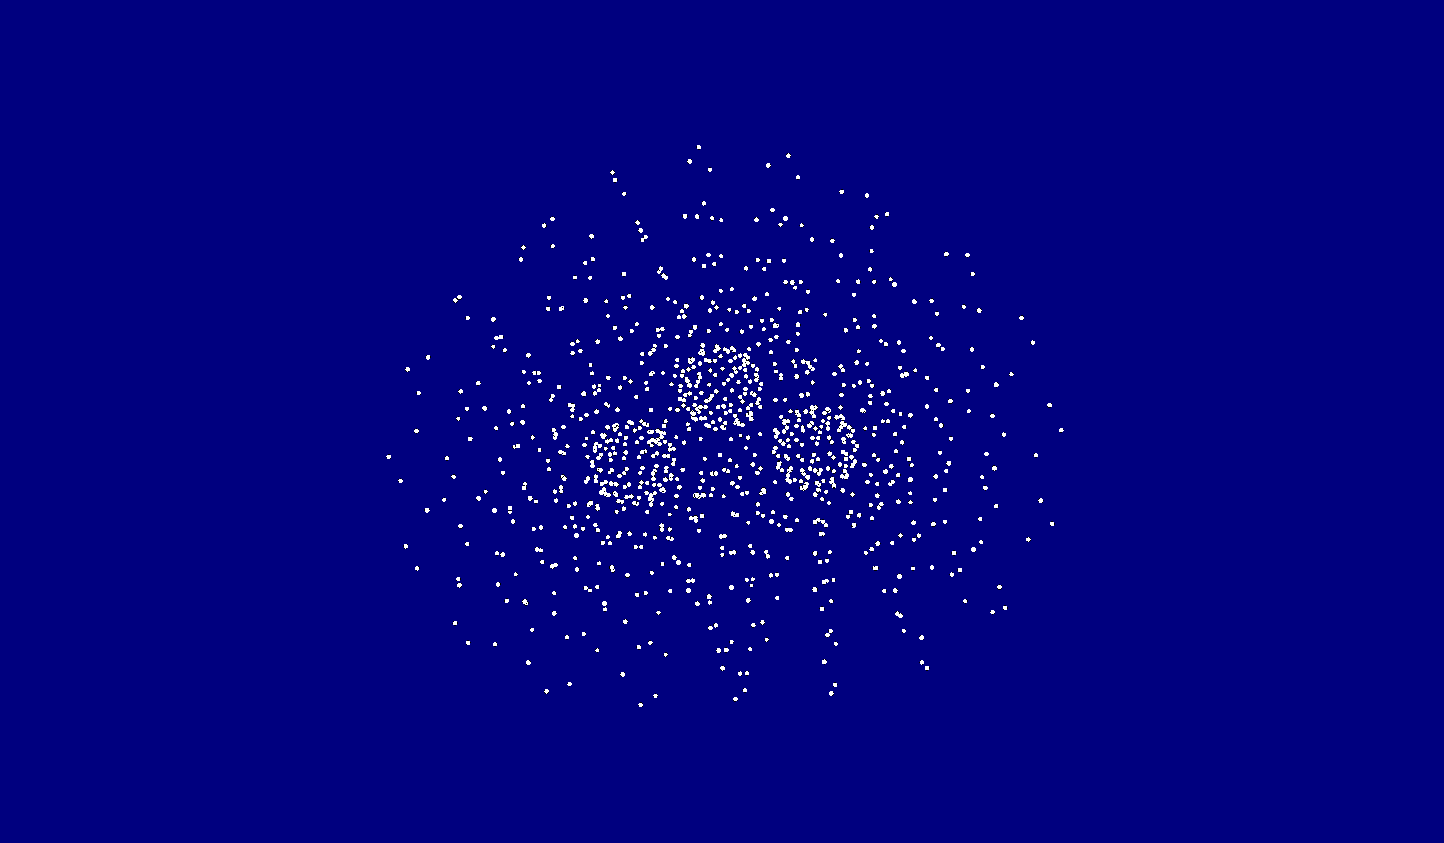
\includegraphics[width=0.5\textwidth]{water1}
   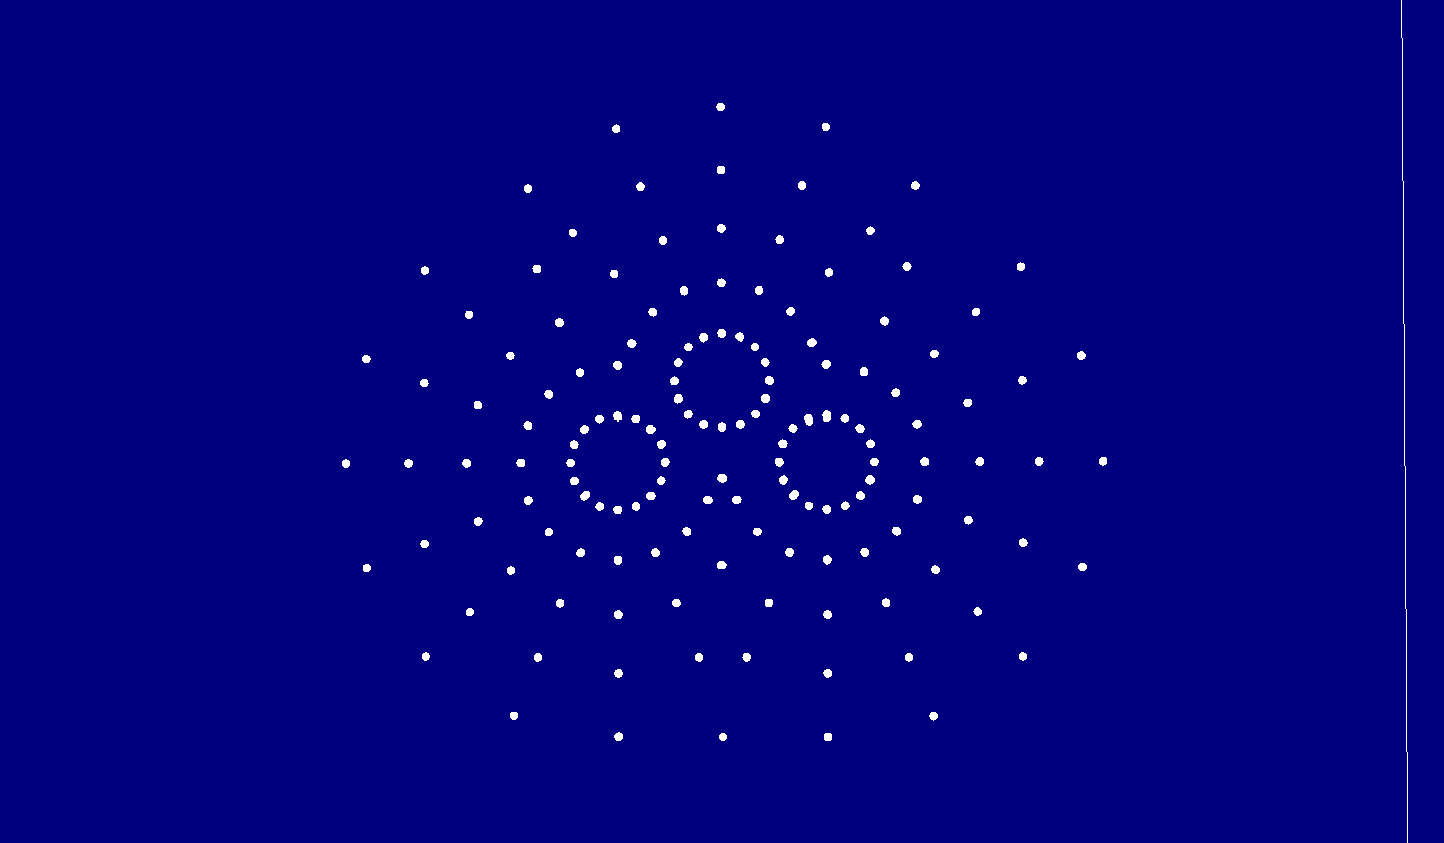
\includegraphics[width=0.5\textwidth]{water2}
   \caption{Example of a mesh for the water-geometry. It consists of $5$ spheres with constant number of points per sphere. The overlapping regions are cut off. Left: cut through the nuclear plane. 
   \textcolor{red}{add figure with distribution: tm}}
   \label{fig:molmesh}
\end{figure}

For the radial distribution of $N$ spheres Son and Chu \cite{Son_Chu0} suggested the scheme
\begin{equation}
r_i=\frac{il}{N-i+\frac{lN}{r_\text{max}}} \qquad i=1,\hdots ,N 
\end{equation}
where $l$ is a free parameter.
As an alternative distribution, in this work the formula
\begin{equation}
r_i=\frac{il}{\left( \frac Ni \right)^p \left(\frac{Nl}{r_\text{max}}-1\right) +1} \qquad i=1,\hdots ,N 
\end{equation}
is suggested where two degrees of freedom $l$ and $p\geq 1$ are given and the condition $N<\frac{r_\text{max}}{l}$ needs to be fulfilled to prevent the singularity.
%Thereby it is important to mention that in this scheme (in contrast to the above one) the (asymptotic for $r\rightarrow \infty$) maximum distance between two spheres is $l$ and hence could be physically chosen to $l\approx \frac \lambda 2$.

While the distribution of spheres follows, at least on a qualitative level, a clear scheme since it should always resemble the local kinetic energy, the distribution of points on the surface of each sphere more complicated.
Here, a regular distribution is a good choise, but on the non-linear topology of the sphere, regularity is in general more challenging.
While so-called geodesic grids are popular in earth sciences \cite{geodesic1,geodesic2,geodes_charge}, their construction allows only for exponentially growing mesh-sizes.
Another common approach is to use quadrature points of integration rules of a given order which lead to Lebedev-grids \cite{lebedev,lebedev2} and spherical t-designs \cite{t-design1, t-design2} that are found more often in quantum chemical contexts \cite{LebQC1,LebQC2,lebDFT,lebDFT2} and will be used in this thesis.
Further methods involve the search of extrem such as minimisation of the Riesz s-energy, and other geometric properties \cite{fliegeMaier,womersley,wom2,wom3} or a set of qualitatively lower but computationally much easier schemes such as the spherical fibonacci mapping \cite{fibonacci,fibonacci2}.

Since in finite element theory the sphere neither needs to be really round nor is there any global functional defined on it,
the complicated distributions described above may be not even needed. 
An other approach therefore is to use an algorithm that gives just a more or less uniform distribution.

%Some explanations are given here:\\ %https://www.maths.unsw.edu.au/about/distributing-points-sphere
%Approach used for climate models: so-called geodesic grids: subdivision of polyhedra, projected onto the sphere\cite{geodesic1, geodesic2}, see also
%http://kiwi.atmos.colostate.edu/BUGS/geodesic/
%http://kiwi.atmos.colostate.edu/BUGS/pdf/ZM-grid.pdf
%http://kiwi.atmos.colostate.edu/BUGS/pdf/conservation.pdf
%http://kiwi.atmos.colostate.edu/BUGS/pdf/ccsr.pdf

The above mentioned techniques show the large variety of different approaches and it is not very clear which one will meet our needs best.
Moreover, here the problem is not only two dimensional but the whole sphere (not only its surface) needs to be subdivided. 
Hence, besides the question of a radial density of different spherical surfaces, also the number of points per sphere as function of the radial distance 
needs to be considered.

Whether the approach of subdividing the atomic meshes into radial and angular parts as opposed to another volume tessellation can be questioned and 
may turn out to be inefficient.
Application of Geodesic grid in calculating surface charges: \cite{geodes_charge}, also mentioning Connolly algorithm (refs 26, 29 therein).

The second scheme has a divergence around $Nl=r_\text{max}$. 
It can be shown that the condition $N\leq \frac rl $ is enough here to stabilise it.

%\textcolor{yellow}{
%If the above described procedures prove to be too inefficient, one could try to implement some WKB-based scheme similar to \cite{impLDVR} but in 3D.
%Thereby, the number of points in a given volume element is determined by $N_i=\frac{\alpha_i}{\alpha} N$ where $\alpha=\sum_i \alpha_i $ and
%\[ \alpha_i= \int_V dV \sqrt{2\mu (E-V(r))} \]
%.This ensures dense points there, where the potential is lowest and a coarse mesh far away; however, a consistent formulation in 3D would need to be invented.
%}

To account for the molecular geometry and the general tendency of the photo electron to oscillate stronger in the vicinity of the nuclei, the mesh is built out of spheres, centred at the nuclear positions.
Thereby, a study of Son \cite{Son_Chu0} had shown that it is numerically most efficient when the overlapping regions of these spheres are cut out.
Figure \ref{fig:molmesh} shows an example for the water molecule.

For the radial distribution we will use the the function
\[
r_i = \frac{1+x_i}{1-x_i+\frac{2L}{r_{max}}} L \qquad x_i = \frac{2i}{N_r} -1
\]
suggested by Son \textit{et. al.}\cite{Son_Chu0, Son_Chu}.
The parameters $N_r$, $L$ specifying the number of spheres and their distribution; the larger $L$ is, the denser are the spheres close to the centre.

The optimal choice of these parameters as well as the angular distribution of points on the spheres is still an open question.
Finally, after putting the points together as described above, they are connected to a Delaunay triangulation using \prog{tetgen} \cite{tetgen}. 
Here additional points may be introduced to guarantee well-shaped elements (\texttt{i.e.} no sharp peaks).

One scheme suggested by Son and Chu \cite{Son_Chu0}:
\begin{equation}
r_i=\frac{il}{N-i+\frac{lN}{r_\text{max}}} \qquad i=1,\hdots ,N 
\end{equation}
where $l$ is a parameter to chose.
Own scheme:
\begin{equation} \label{eq:tm_map}
r_i=\frac{il}{\left( \frac Ni \right)^p \left(\frac{Nl}{r_\text{max}}-1\right) +1} \qquad i=1,\hdots ,N 
\end{equation}
where $l$ and $p\leq 1$ are parameters to chose. Thereby it is important to mention that in this scheme (in contrast to the above one) the (asymptotic for $r\rightarrow \infty$) maximum distance between two spheres is $l$ and hence could be physically chosen to $l\approx \frac \lambda 2$.

The second scheme has a divergence around $Nl=r_\text{max}$. 
It can be shown that the condition $N\leq \frac rl $ is enough here to stabilise it.

Besides the tricky question about this mapping, also the number of points per sphere depending on the radial distance should be considered. 
In \cite{Son_Chu0} this is chosen to be constant without further discussion but of course there are several possible design criteria as well.
Besides a constant number, also a constant spherical density (hence $N\propto r^2$) are possible; However, it might be sensible to follow a similar idea than in the radial mapping: Being fine close to the nuclei and get coarser with increasing distance.
In particular, I followed the design rule of keeping the space between points in radial direction similar to space between points in angular distribution.
Hence, $d_\text{spheric}=\sqrt{\frac{4\pi r_i^2}{N_i}}\approx r_i-r_{i-1}$.
For the above described radial schemes, this results in 
\[
N_i= \frac{4\pi}{ \left(1-\frac{i-1 }{i}\frac{N-i+\frac{lN}{r_\text{max}}}{N-i+1+\frac{lN}{r_\text{max}}}\right)^2 }
\]
for the first scheme and 
\[
N_i= \frac{4\pi}{\left(1-\frac{i-1 }{i}\frac{ (\frac{N}{i})^p \left(\frac{lN}{r_\text{max}}-1\right)+1}{ (\frac{N}{i-1})^p\left( \frac{Nl}{r_\text{max}} -1 \right) +1 } \right)^2 }
\]
for the latter.

The respective radii and number of points per sphere are shown in figure \ref{fig:maps}.\\
Special mapping schemes are the constant radial mapping $r_i=a i$ which corresponds to a constant spherical grid density $N_i=4\pi a^2 i^2$ and an exponential map $r_i=q^i r_0$ which would require a constant number of spherical grid points $N_i=\frac{4\pi q^2}{(1-q)^2}$ according to the rule derived above.

\begin{figure}
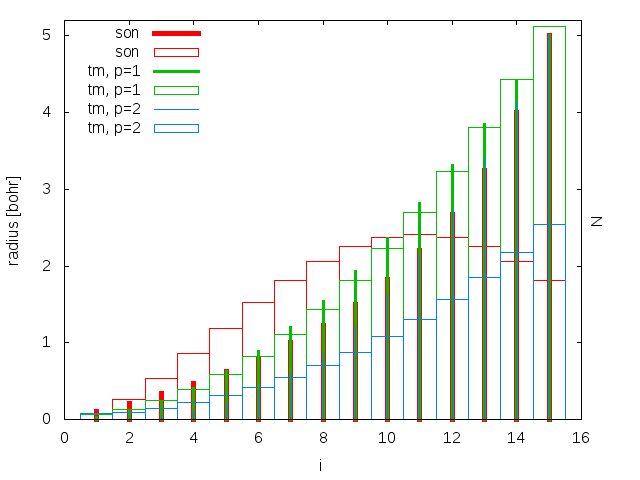
\includegraphics[width=0.7\textwidth]{Figures/RadialMap}
\caption{the radius and number of points of the spheres as for $N=15$, $r_\text{max}=5$ and $l=2$.}
\label{fig:maps}
\end{figure}

Since some of the spherical schemes described above allow only for certain numbers of points each, here, the best approximation is used respectively.

\subsection{Obtaining ESP}
 - obtained from \prog{NWChem}
 - interpolation of that grid

\section{Obtaining the DOs}
 - from coefficients to values


\chapter{Results and Discussion}
\label{ch:res}
In the previous chapters, many different methods that can be used to compute PESs numerically are described and in chapter \ref{ch:proced} the method used within this work is described in more detail.
In this chapter some results are shown and explained.

Since the method developed in this work combines several techniques that have not been used together so far and several conceptual questions need to be clarified before computing actual PESs, is section \ref{ch:BCbench} two BCs are compared in their influence on the wave-function. In section \ref{sec:NumConve} further benchmarking calculations on some numerical parameters are shown.
For simplicity, these calculations were performed using a Lithium atom as test system.

In section \ref{ch:resLI} further results for atomic Lithium are presented, showing several conceptual ... .

%There is a paper\cite{vibPES} with vibronically resolved PES from experiment.\\
%PES of N2 with 'angular resolution' (latter not directly) \cite{PESN2}.
%purine and pyrimidine: comparison to Green's function methods via the \cite{PottsHolland}-paper.
%For AlO$^-$ there is a paper with 2 spectra with one and two transitions each, having vibrational
%structure\cite{AlO}.
%Atomic Systems have some experimental data as well: For Xe and Kr the spectra at photon energies of 150$\,$eV are shown in reference \cite{KrXe}.
%A combined theoretical and experimental study on CH$_2$F$_2$ is in ref. \cite{ch2f2}. Here, theory is quite bad and experiment is also angular resolved, thus may be interesting.

\section{Comparison of Boundary Conditions}
\label{ch:BCbench}
In section \ref{ch:BC}, many BCs which give rise to diverse properties for the solution are briefly described.
Detailed comparisons of some of these BCs are studied in various works \cite{babuska,artBC,capComp,absRev,nrBCrev} for several systems.
For simplicity, here only two BCs are studied in more detail.
First, in section \ref{sec:DBCbench} several properties of the grids introduced in section \ref{sec:grid} are studied with Dirichlet boundaries which are particularly easy to set up and understand in their physical consequences.
In section \ref{sec:iBCbench}, several properties of the mesh with infinite elements are investigated.
Since it turns out that the solutions obtained with infinite elements are very sensitive to the parameters, this study is performed more extensively.
For simplicity, the tests shown here are on atomic systems using, unless specified otherwise, an analytic Coulomb potential with charge $1$, corresponding to the ionised hydrogen atom.

\subsection{Dirichlet Boundary Condition}
\label{sec:DBCbench}
Dirichlet boundaries are conceptually the easiest BCs but are known to have a large influence on the solution, especially for continuous functions since they reflect outgoing waves fully.
%\begin{wrapfigure}{l}{0.6\textwidth}
%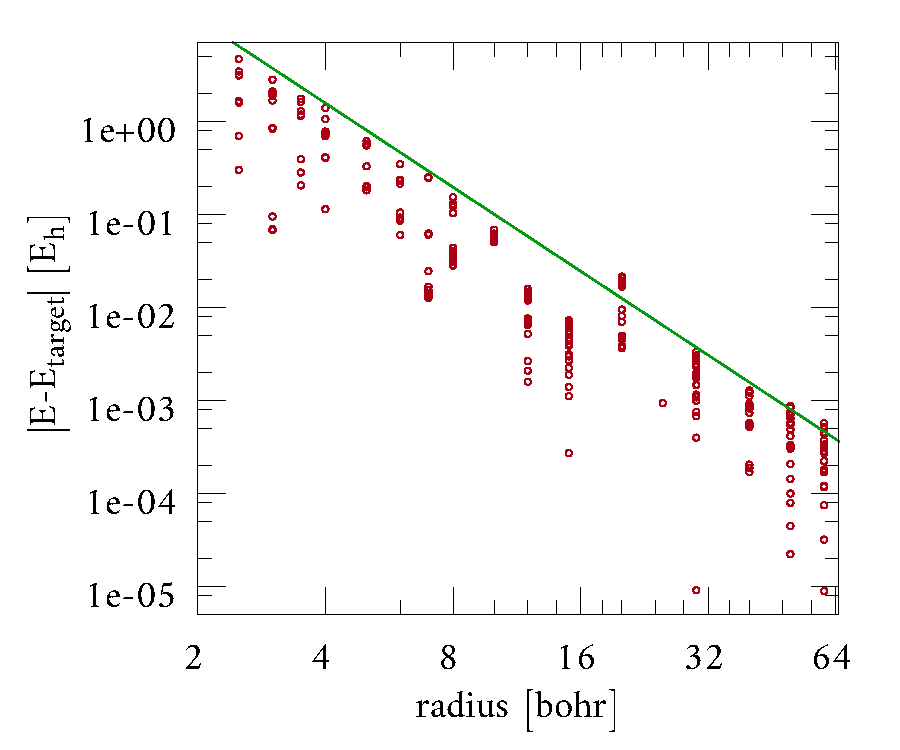
\includegraphics[width=0.6\textwidth]{Figures/BC/DBCenergies}
%\caption{double-logarithmic plot of the error in energy of the energetically closest solutions in dependence on the radius
%of the sphere. The comparison with $\propto \frac{1}{r^3}$ shows the general behaviour of the error.}
%\label{fig:dbcRad}
%\end{wrapfigure}
\begin{figure}
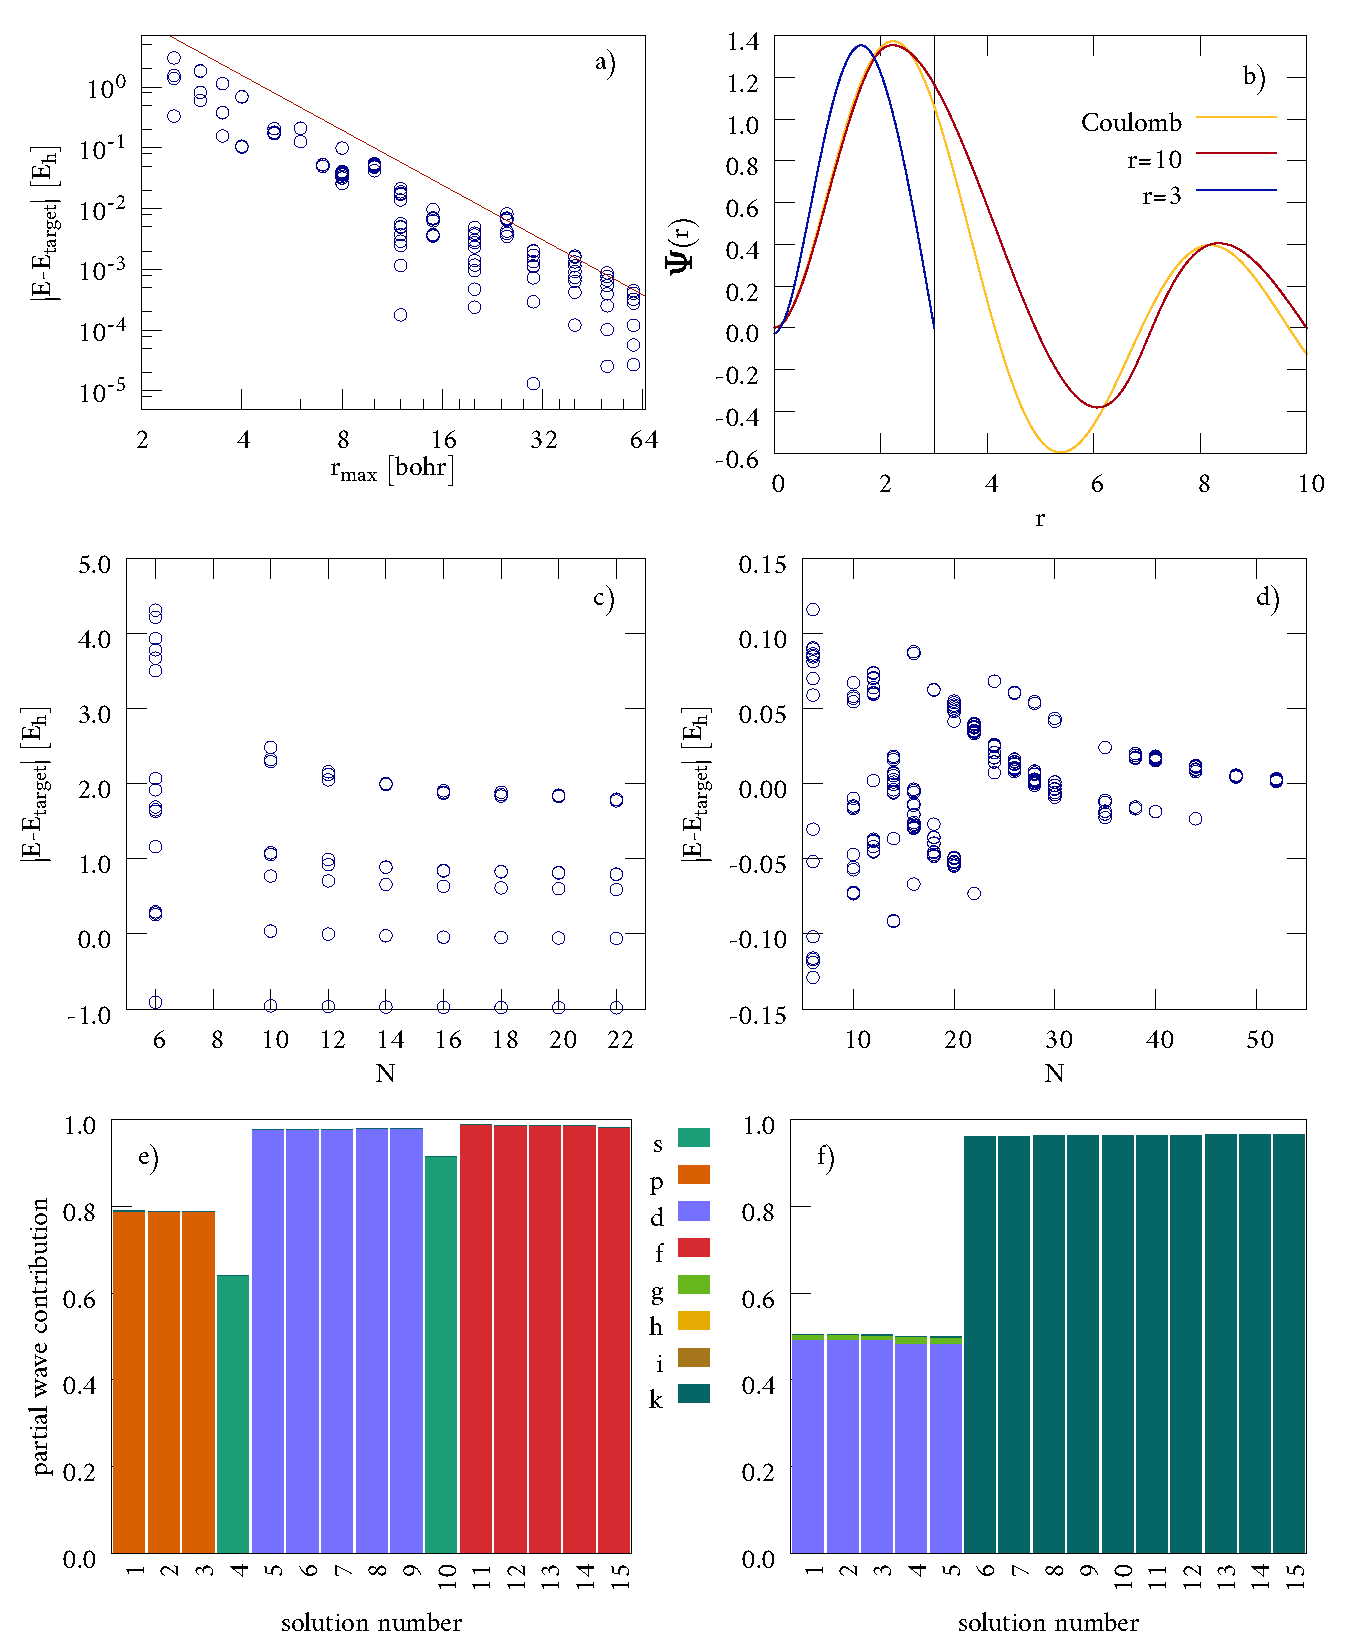
\includegraphics[width=\textwidth]{Figures/BC/DirichletBC}
\caption{Several properties of the solutions obtained with Dirichlet BCs using different box sizes:\\
a) double-logarithmic plot of the error in energy of the energetically closest solutions in dependence on the radius
b) radial part of $d$-wave functions obtained with different box-sizes( $r=4$, blue line and $r=10$, red line); Coulomb wave (yellow line) for comparison.
c) and d) plot of the error in energy for radii of $4\,$bohr, and $10\,$bohr,\ varying the number of spheres in the box
e) and f) show the partial wave coefficient (\ref{eq:PartWaveCoeff}) of different angular momenta of the respective solutions with $r=4$ and $N=16$ (left) as well as $r=10$ and $N=38$, respectively.}
\label{fig:dbcRad}
\end{figure}
Moreover, its requirement for the solutions to vanish at the boundaries results in an artificial discretisation of the radial solution similar to that of bound states which leads to a banded spectrum with a size-dependent energy gap between two states with same angular momentum.
Moreover, these boundaries enforce the real and imaginary part of the solution to be identical up to symmetry operations (such as rotations and reflections for spherical systems) which does not hold for continuum waves such as Coulomb waves as can be seen in Figure \ref{fig:RadFun} and plane waves that have a constant phase shift.

These properties are found in various tests conducted to find reasonable parameters for application to more complex systems.
In Figure \ref{fig:dbcRad} a), the error in the energy of $20$ solutions is shown for different radii.
The comparison with the red line that represents a cubic decay, shows that the error is inverse proportional to the volume of the box which is a well-known result for particles in a box with infinite potential walls. 
The number of spheres is kept constant at $N=20$.
The influence of the number of spheres on the energies is shown in the panels c) and d) of Figure \ref{fig:dbcRad}.
In these figures several branches of solutions can be seen that correspond to different angular momenta.
For smaller radii ($r=4$, panel c)), these branches are well-separated but become closer and finally interfere with each other at larger radii ($r=10$, panel d)) where also strong coupling of angular momenta can occur.
Following the expectations, the energies of the respective branches decay when the number of degrees of freedom is increased.
The lowest panels in Figure \ref{fig:dbcRad} show the contributions from plane wave functions with respective kinetic energy and different angular momentum where the partial wave coefficient is defined as
\begin{equation} \label{eq:PartWaveCoeff}
|\langle \Psi_\text{num} | \Psi_{\vec{k}}^\text{Sph}\rangle |^2
\end{equation}
where $|\Psi_{vec{k}}^\text{Sph}\rangle$ is the spherical wave (\ref{eq:spherWave}) and $|\Psi_\text{num}\rangle$ denotes the respective numerically obtained solution.
For numerical reasons, here the comparison is done against the spherical waves and not against Coulomb waves.
In Figure \ref{fig:dbcRad} b), two solutions with $l=2$ along one axis are shown (the fifth one for $r=4$ and the first one for $r=10$) for two different box-sizes and compared to the Coulomb wave.

However, the density of solutions is not the only important quantity: To obtain reasonable intensities, the respective angular momentum is more important to obtain reasonable results.
Respective tests show that for a given energy of the photoelectron of $E=0.566\,$ Hartree the obtained solutions have a well-defined angular momentum only for small boxes where the critical radius is in the order of $r_\text{max}=10\,$bohr.
For larger meshes, the states have large contributions from different angular momenta and are very sensitive to different parameters such as the number of spheres $N_i$ and the parameters $p$ and $q$ of the distributions of the spheres (\ref{eq:tm_map}) and (\ref{eq:son_map}) respectively.
Moreover, for example the comparison of the Figures \ref{fig:dbcRad} e) and f) shows that solutions on larger meshes tend to have higher angular momenta which is an important argument in favour of smaller boxes since for most atomic systems angular momenta larger than $4$ are not of interest.

%\subsection{Complex Absorbing Potential}
%Using a CAP as described in section \ref{ch:cap}, two additional degrees of freedom comared to the Dirichlet BCs arise: the strength $\eta$ of the artificial potential (\ref{eq:cap}) and the offset $r_0$ where it starts, the latter has the only restriction to be larger than the radius of the DO.
%In section \ref{ch:cap} it was suggested to chose the parameters such that the respective derivatives of the energy vanish \cite{CAPccEOM,CAPfreshlook}.
%This procedure is, however, only valid if one solution should be taken into account and thus is not directly applicable here.
%Interpreting the real part of the eigenvalues of the eigenproblem (\ref{eq:SEmat}) as the energy of the respective state, the influence of the CAP on the density of states varies strongly when changing other parameters.

\subsection{Infinite Elements}
\label{sec:iBCbench}
In section \ref{ch:InfEl}, several formulations of infinite elements are presented.

which require some investigation to get an understanding of the properties of the numerical setup described so far.
Among these questions is the formulation of infinite elements, discussed in section \ref{ch:InfEl} of which the most important ones are studied in section \ref{ch:bmFormul}.
\begin{wrapfigure}{L}{0.5\textwidth}
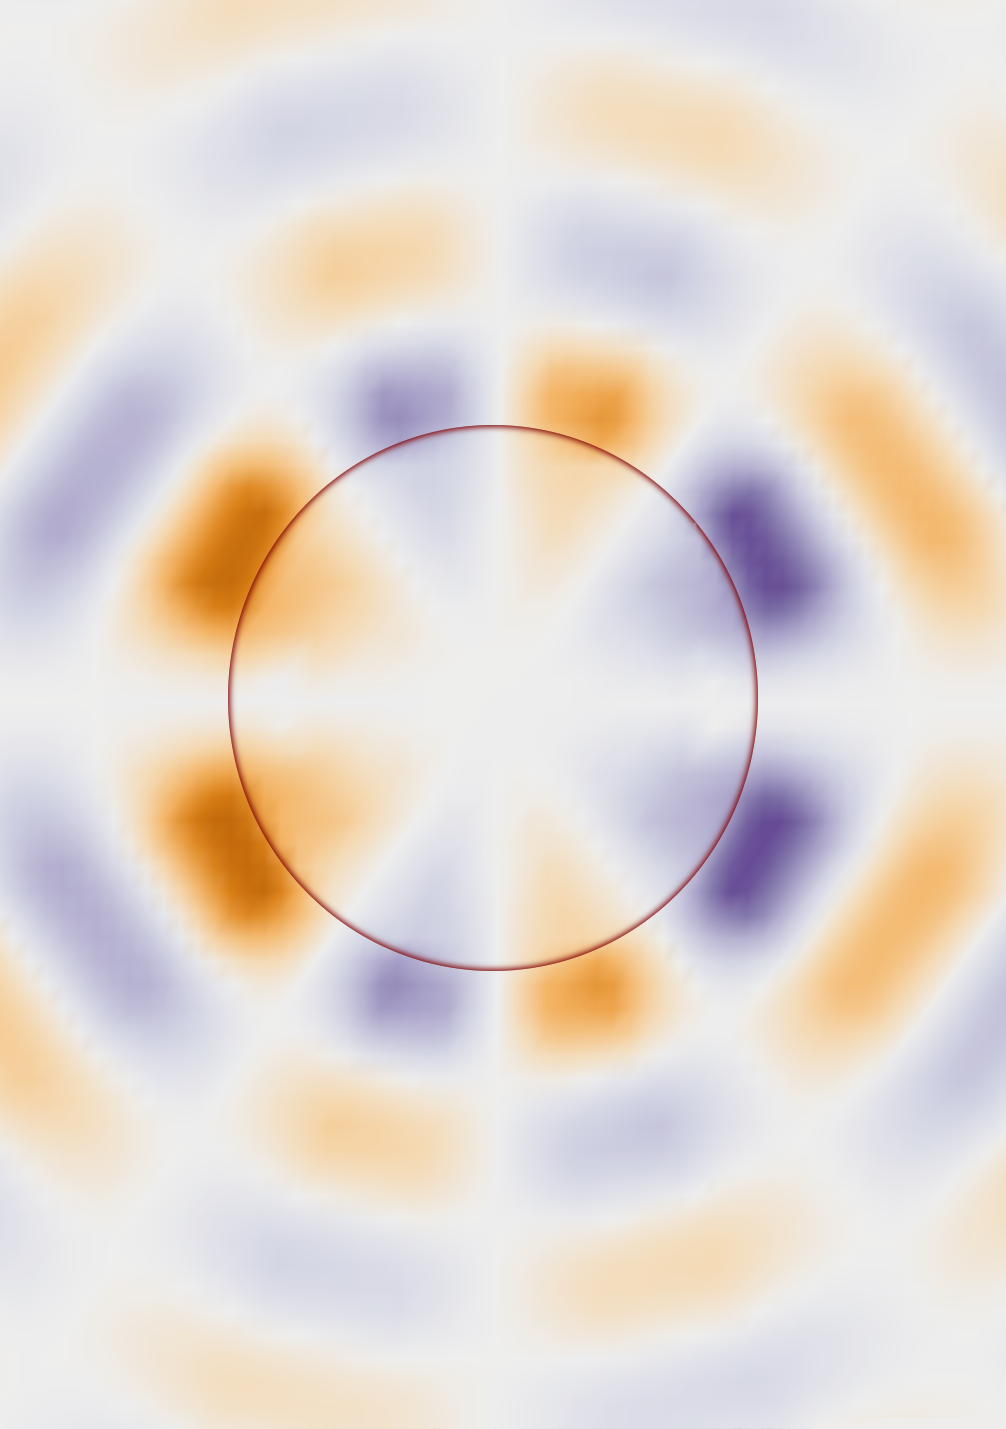
\includegraphics[width=0.5\textwidth]{Figures/BC/plane_fin}
\caption{2D-cut of a solution with infinite elemnts using a spherical finite element region indicated by the red circle with a radius of $r=6\,$bohr and $N=11$ spheres.}
\label{fig:cutInf}
\end{wrapfigure}
In Figure \ref{fig:cutInf}, a 2D-cut of a solution obtained with infinite elements for the Hydrogen atom is shown, the red circle indicates the region of finite elements.
The features shown in Figure \ref{fig:cutInf} are prototypic for the properties that are found for the infinite elements here.
It is clearly visible from the graph that the infinite region resembles the asymtotic behaviour, showing the expected regular oscillations of an outgoing wave.
However, the angular momentum is quite large, leading to only small contributions in the finite element region.

%\subsubsection{Formulation of Infinite Elements}
\subsubsection{Comparison of Formulations}
\label{ch:bmFormul}
Before having a closer look at the convergence of different parameters, first the formulation of infinite elements to be used later is investigated.
Since the unconjugated Burnett-formulation was not very successful \cite{dreyer}, the conjugated formulations of Burnett and Astley-Leis both have interesting features to use for quantum mechanical problems.
Since the conjugated Burnett elements lead to infinitely large matrix elements, here the Astley-Leis elements (\ref{eq:ALelem}) are compared with the symmetrised form (\ref{eq:ALsymm}) using different powers $p$.
Moreover, to study the influence of the damping function in the Astley-Leis formulation (\ref{eq:ALelem}) in more detail, also a test function space similar to eq. (\ref{eq:ALelem}) but using the squared damping function $D(r)^2$ instead of $D(r)$.

The 50 real solutions whose energy is closest to the target value of $15.44\,$eV ($0.5675\,E_h$) obtained with the original Astley-Leis formulations with the damping function taken to the powers $p=1,2$ as well as the symmetrised formulation (\ref{eq:ALsymm}) suggested in this thesis with powers $p<0.5$ are shown in Figure \ref{fig:IFEMform_spect}.
For the unsymmetric formulations only the real part is shown which is assigned to the physical energy of the respective state.
\begin{figure}
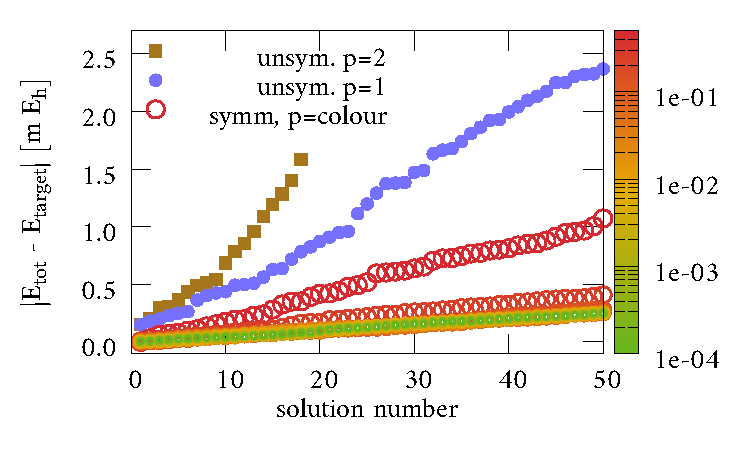
\includegraphics[width=\textwidth]{Figures/IFem_form_spectra}
\caption{The first 50 eigenvalues obtained with the original Astley-Leis formulation (imaginary part not shown) and with the symmetrised form (\ref{eq:ALsymm}).}
\label{fig:IFEMform_spect}
\end{figure}
The results shown in Figure \ref{fig:IFEMform_spect} show clearly that the obtained density of states decreases with the power $p$ and converges for $p\approx \frac 18$ for the given parameters (the radial mapping scheme (\ref{eq:tm_map}) is used with $N=25$, $l=0.5$, $p=2.5$ and $r_\text{max}=7\,$bohr.).

The dependence of the obtained spectrum of the Hamiltonian on the power of the damping function shows that, at least for FEFs, the asymptotic behaviour is crucial for the properties of the wave function. 
The dependence converges for $p=1/8$, see also Figure \ref{fig:powerSpect} in supplement.
Moreover, even for small powers $p\approx 10^{-4}$, no numerical instabilities are observable so that there is some freedom in this parameter and it does not need to be optimised for different systems individually.
The observations made on the convergence-properties using the spectrum in Figure \ref{fig:IFEMform_spect} are supported by the projections of the solutions on spherical waves of which some are shown in Figure \ref{fig:IFEMform_project}.
\begin{figure}
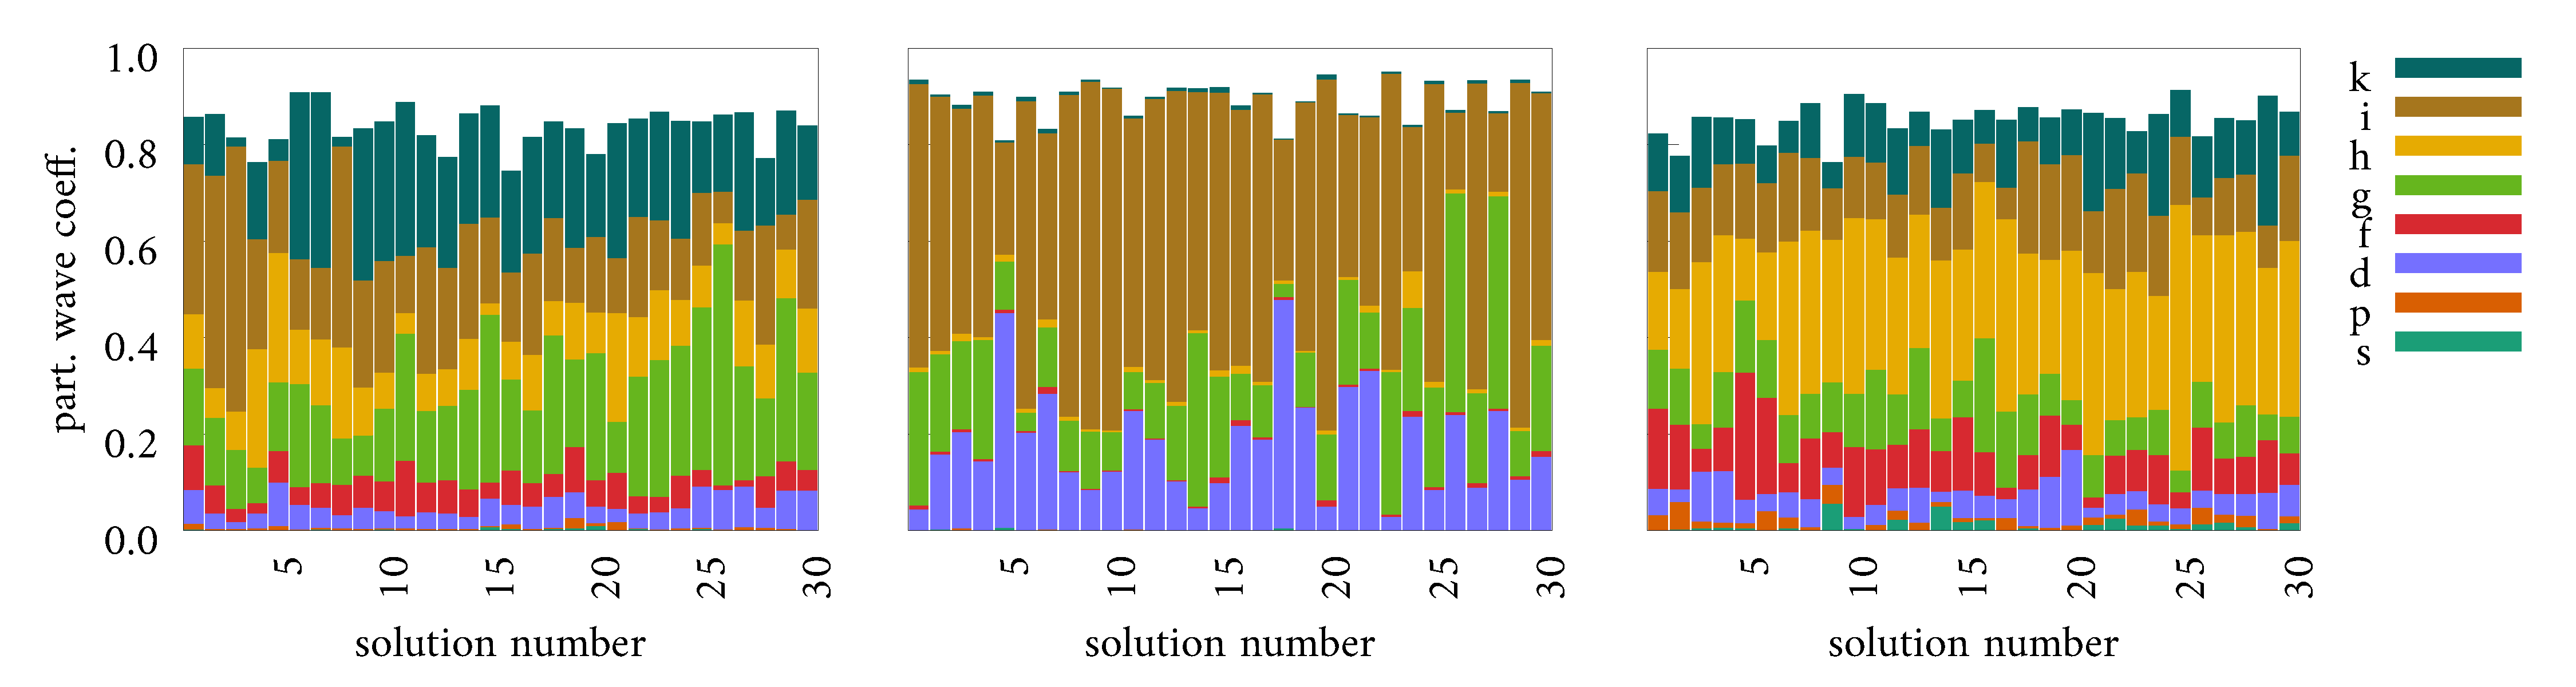
\includegraphics[width=\textwidth]{Figures/Ifem_forms}
\caption{Decomposition of the first 30 solutions into spherical waves with angular momenta up to $l=7$.
Left: Astley-Leis-formulation ($p=1$), middle: symmetrised form ($p=0.5$) right: symmetrised form ($p=10^{-4}$).}
\label{fig:IFEMform_project}
\end{figure}

As shown in the Figure \ref{fig:IFEMform_project}, the nature of the states obtained is in all cases strongly mixed in the quantum number $l$ with significant contributions even for $l>7$.
However, the relative contributions of the angular momenta critically depends on the power $p$, making a reasonable choice of this parameter important.
Further it is expected that the convergence of $p$ depends on further parameters such as the box-size and kinetic energy of the photoelectron which is, however, not studied here in more detail.
Instead, in the following the power of the damping function $D$ is chosen to be $p=0.0001$ if not specified differently.
This value is far in the convergence region of Figure \ref{fig:IFEMform_project} and thus is hoped to be reasonable also for other systems.

%\subsection{Size of Finite Element Region}
\subsubsection{Radius of the Finite Element Region}
\label{ch:bmSize}
%More important than the subspace used numerically is obviously the size of the sphere used for the FEM description.
Similarly to the Dirichlet BCs discussed in section \ref{sec:DBCbench}, also for infinite element the size of the finite element region has a strong influence on the solution, even if the dependency is weaker as can be seen in Figure \ref{fig:InfBoxs} where the energy of the energies closest to the target value is plotted for different box sizes.
However, the energy-dependence on the box-size is much weaker than in the case of Dirichlet BCs as the comparison with the $\frac{1}{r^3}$-curve in Figure \ref{fig:InfBoxs} and \ref{fig:dbcRad} (a) shows.
\begin{wrapfigure}{L}{0.6\textwidth}
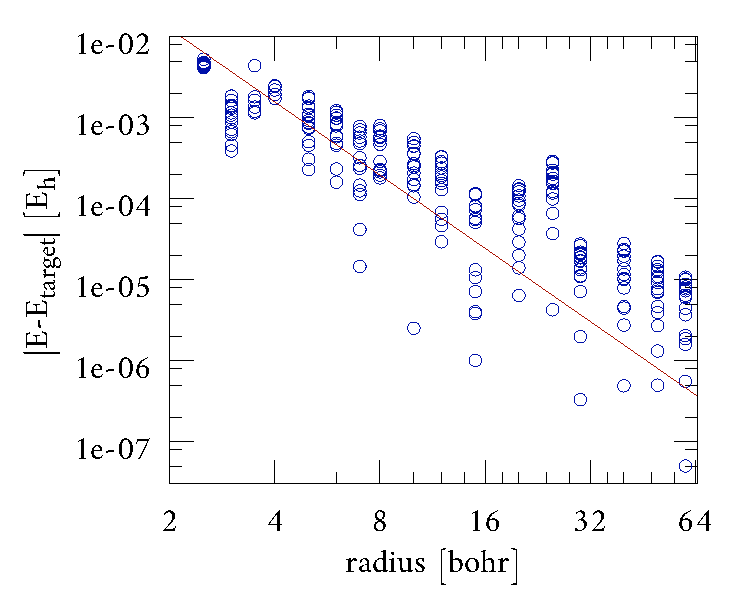
\includegraphics[width=0.6\textwidth]{Figures/BC/BoxsInfEL}
\caption{Double-logarithmic plot of the error in energy for different radii of the finite element region.}
\label{fig:InfBoxs}
\end{wrapfigure}
Moreover, the error in energy is in general much lower with infinite elements which is a further indicate for the higher accuracy of infinite elements compared to the Dirichlet boundaries.
On the other side, also the angular momenta of the solutions are larger than those occurring with Dirichlet BC at the same box-size.
\begin{figure}
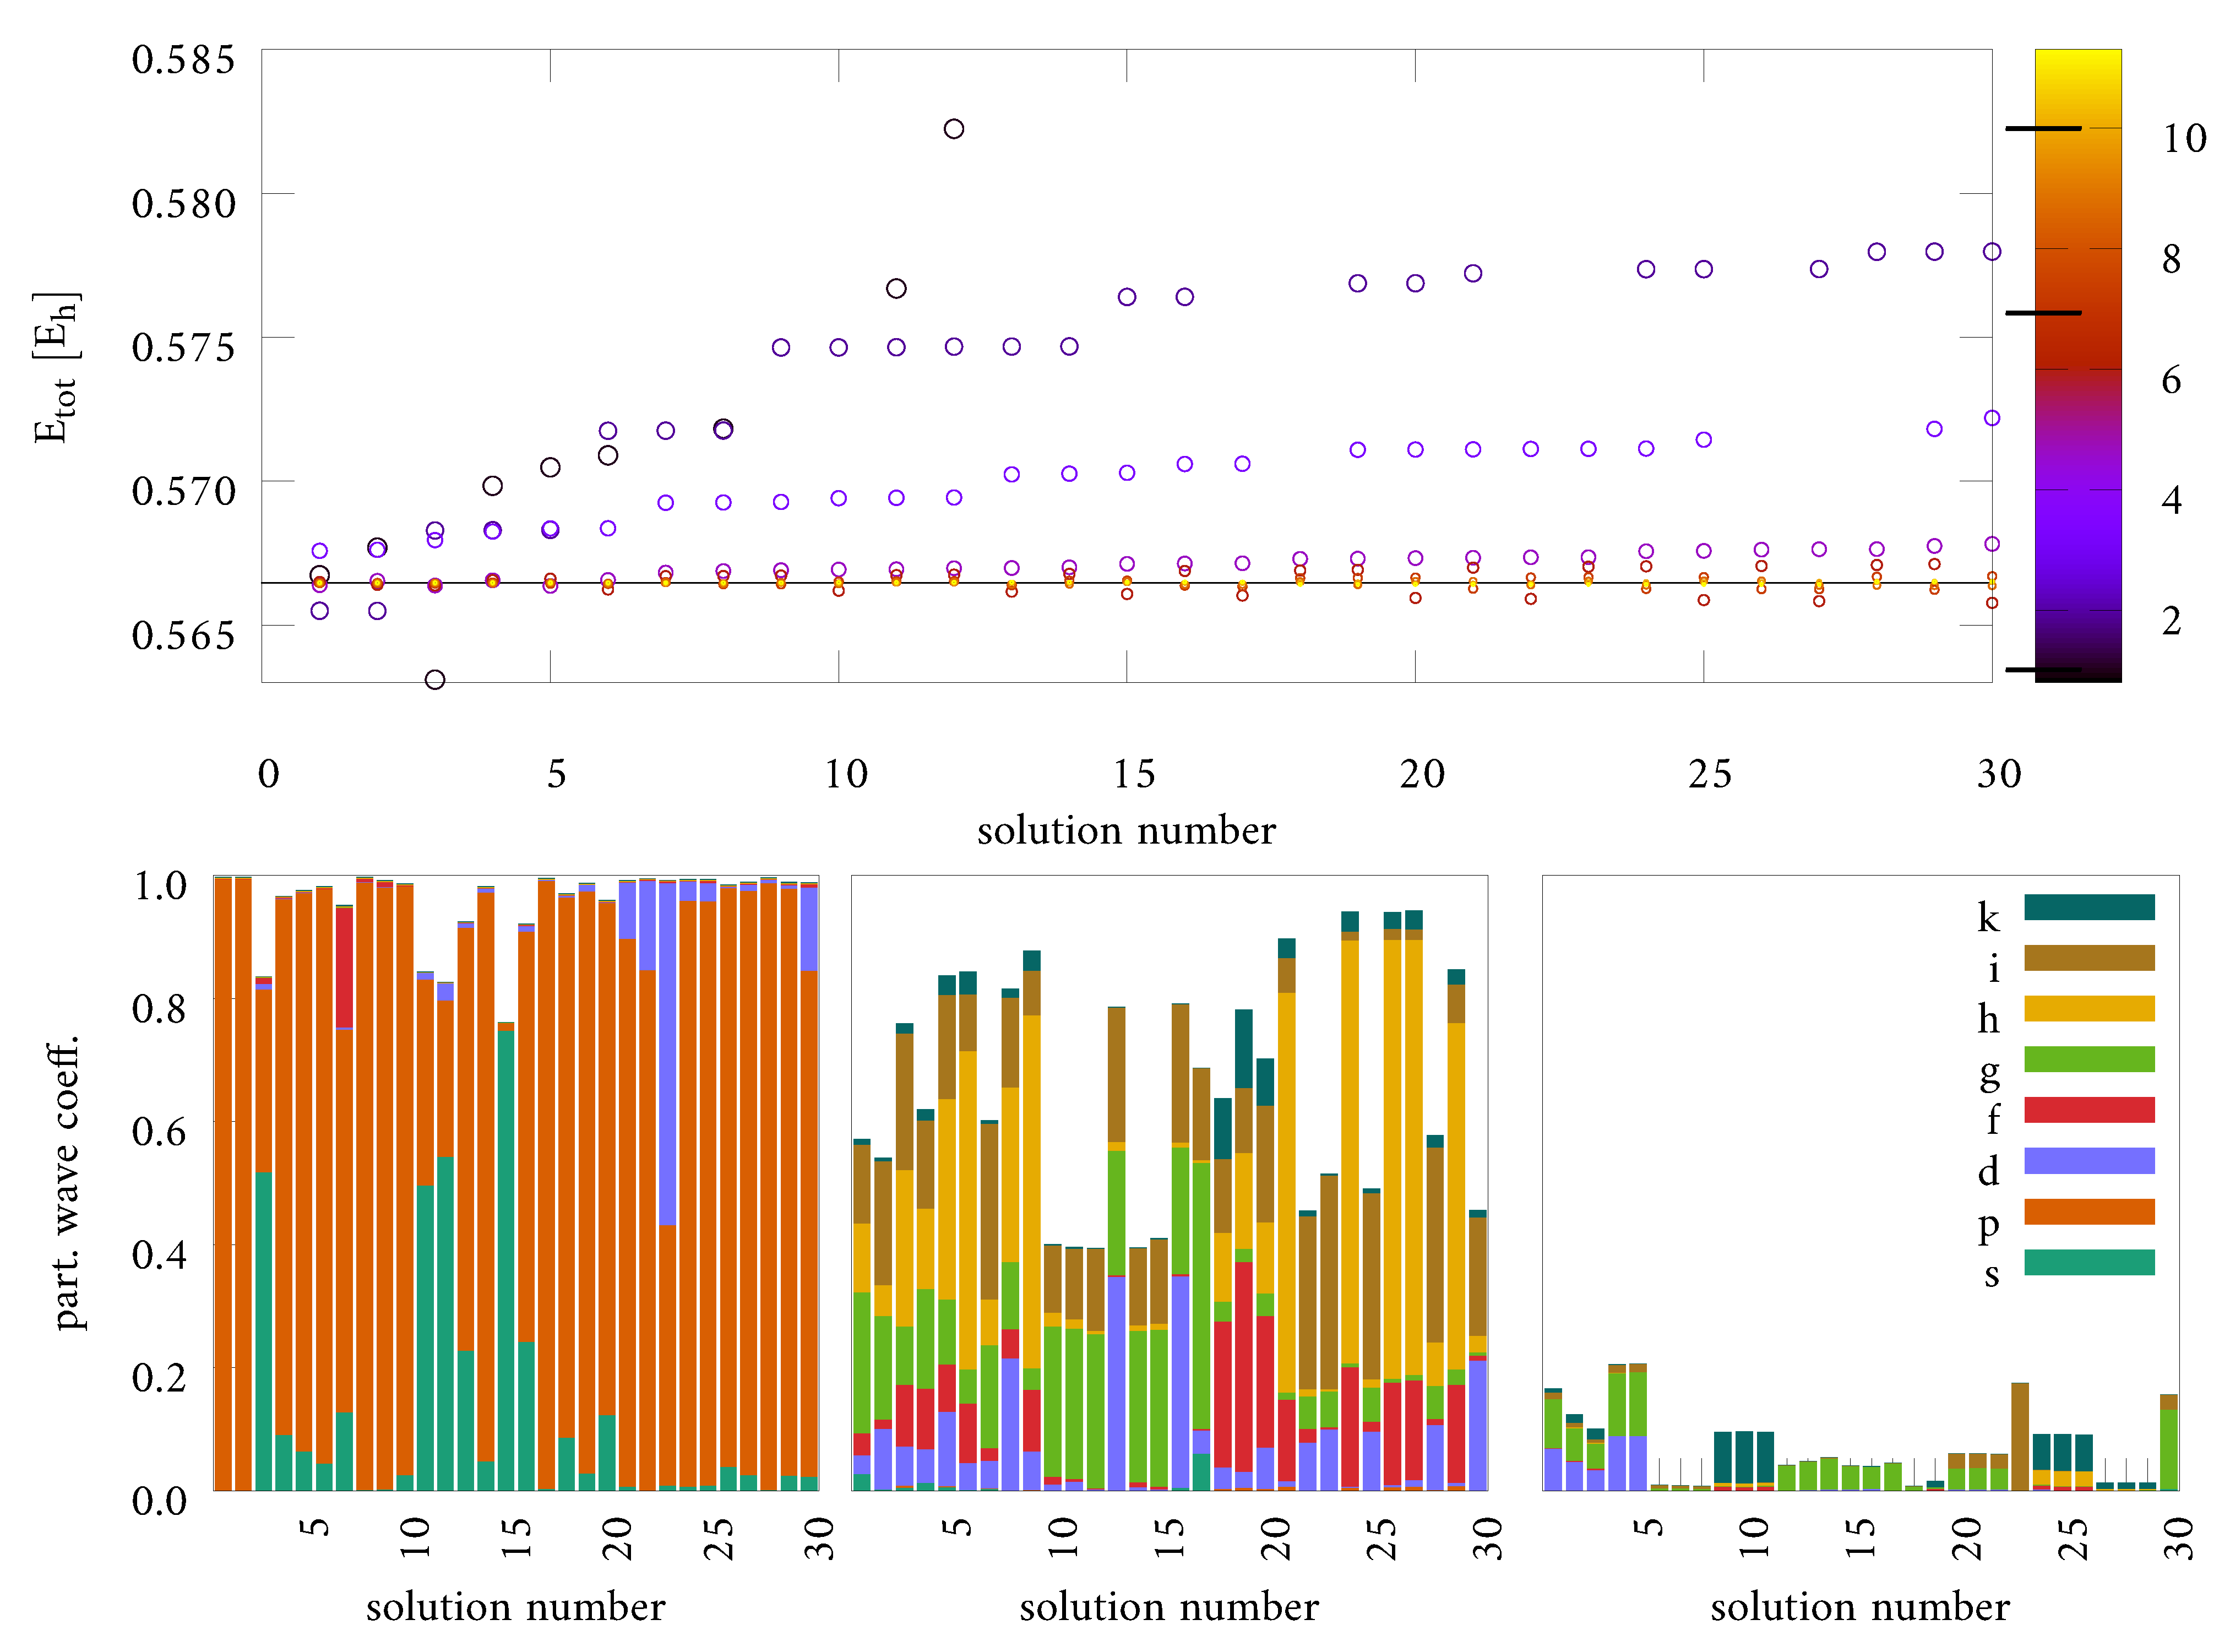
\includegraphics[width=\textwidth]{Figures/RadWave_p0_001.pdf}
\caption{The eigenenergies for different box sizes (coloured dots in the upper panel) where the box size is denoted by the colour in atomic units.
The lower panel shows the decomposition of the solutions into spherical waves for three box sizes, marked by a star in the colour bar respectively.}
\label{fig:RadWaves}
\end{figure}
This behaviour is observed to depend also on the formulation of infinite elements.
Respective tests show, \textit{e.g.}, that the mixing of angular momenta is stronger for smaller damping powers $p$.
This coupling of different angular momenta can be explained by the very density of the spectrum which increases with the radius as shown \textit{e.g.} in Figure \ref{fig:RadWaves} but increases also with descending damping as illustrated in Figure \ref{fig:IFEMform_project}.

This behaviour can be understood when recapitulating the influence of small perturbations (\textit{e.g.} due to numerical cut-off) in form of a matrix $\mat{E}$ of an hermitian matrix to its eigenvectors $\vec{u}_i$ which has the form \cite{saad, wilkinson}
\begin{equation}\label{eq:ErrVect}
\vec{u}'_i=\sum_{j\neq i} \frac{\vec{u}_j^\dagger\mat{E}\vec{u}_i}{\lambda_i-\lambda_j} \vec{u}_j
\end{equation}
where $\lambda_i$ is the eigenvector corresponding to $\vec{u}_i$.
From eq. (\ref{eq:ErrVect}) now the coupling of angular momenta and strong dependence on the parameters for a dense spectrum, \textit{i.e.} small $\lambda_i-\lambda_j$ becomes obvious.

\subsubsection{Density of Spheres}
\label{sec:BenchSphere}
Increasing the number of spheres has, as expected, some influence on the energies but also changes the angular momenta of the solutions.
Similar to the behaviour found for Dirichlet BCs, also when using infinite element BCs a larger number of spheres leads to larger angular momenta as the comparison of the partial wave coefficients in Figure \ref{fig:InfNum} for different numbers of spheres shows.
Moreover, the error of the energy shown on the left side of Figure \ref{fig:InfNum} indicates that the shown configurations are far from saturation.
However, since high angular momenta are not desireable, a smaller number of spheres is better suited even though it is not converged.
Moreover, the behaviour of the properties of the solutions when changing the number of spheres is not very systematic in the range shown.
\begin{figure}
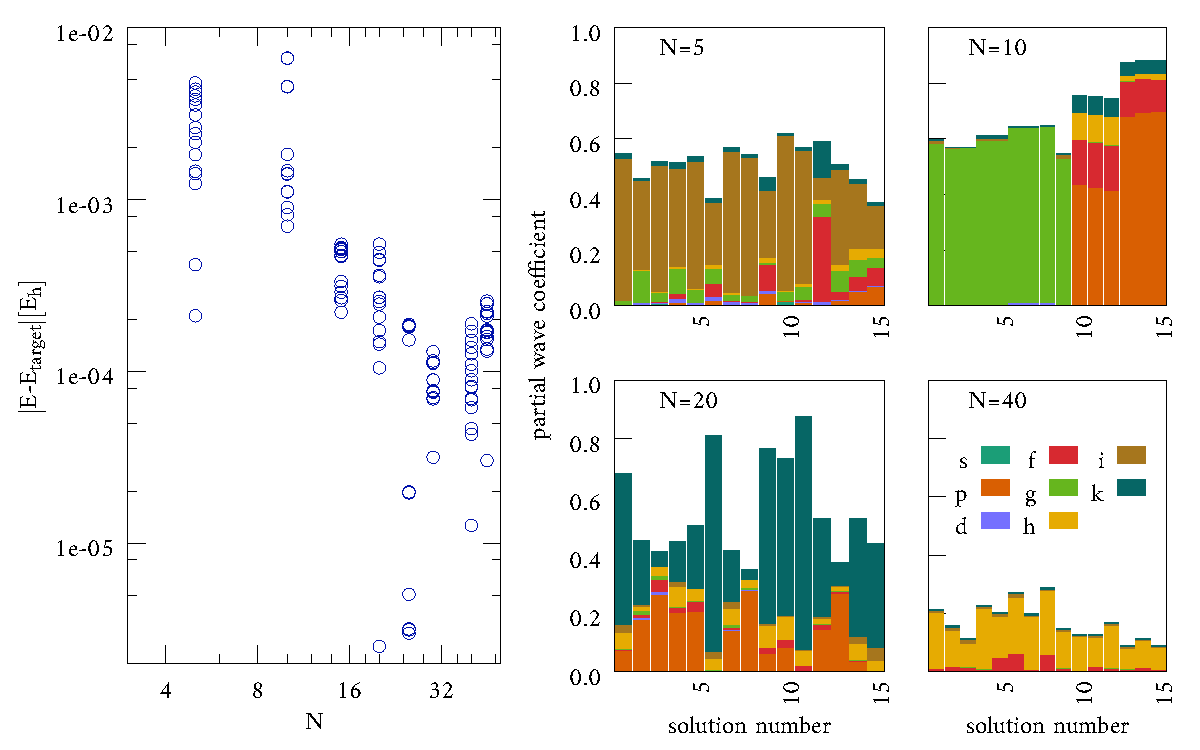
\includegraphics[width=\textwidth]{Figures/BC/NumInfEL}
\caption{The energy (left panel) and partial wave coefficient (\ref{eq:PartWaveCoeff}) for different number of spheres $N$ using infinite elements. The radius is $r=10\,$bohr.}
\label{fig:InfNum}
\end{figure}
As an example, for $N=10$ the energies are much more separated that is reflected also in the angular momenta which show a much weaker mixing than for the other configurations shown.
Not only the unsystematic behaviour, the strong dependence of the angular momentum on the number of spheres as such is surprising since, in principle, the radial and angular nodes should be represented with a similar quality.

\subsubsection{Radial Order}
Using the infinite element scheme, an additional parameter is the order of the radial polynomial $f(r)$ in eq. \ref{eq:Infansatz}.
\begin{figure}
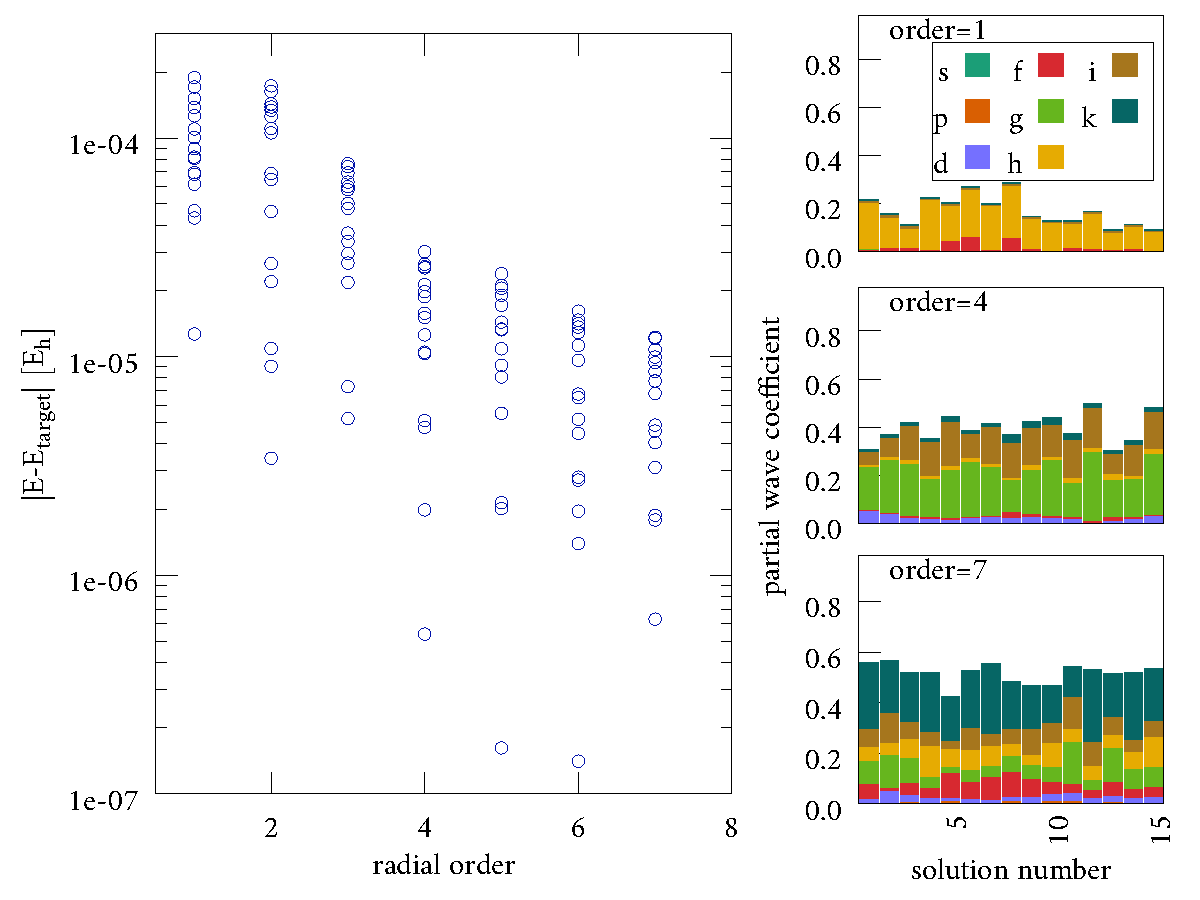
\includegraphics[width=\textwidth]{Figures/BC/OrdInfEL}
\caption{The error in energy for $15$ solutions obtained with a box with radius $r=10$ and $N=40$ spheres using different orders of the multipole expansion $f(r)$, see eq. (\ref{eq:Infansatz}).}
\label{fig:InfOrd}
\end{figure}
The increasing angular momentum with the radial order is, in contrast to the behaviour studied in section \ref{sec:BenchSphere}, not surprising.
As mentioned in section \ref{ch:InfEl}, the  first order infinite element term corresponds to the radial behaviour of an $s$-wave whereas higher radial orders describe the faster decaying waves with respectively larger angular momentum.
Thus, choosing a low radial order ($o=1$) leads to a better representation of low angular momenta and thus is favoured in this context.

\subsection{Conclusion on Boundary Conditions}
The study of different system-parameters presented in the previous sections has revealed several properties of the finite element setup.
An important conclusion of these tests is that a higher density of eigenenergies, which is considered as an indication for a more exact representation of the wave function, in general leads to the appearance af larger angular momenta and, at some point, to strong strong coupling of different angular momenta.
Such a relation is expected for the box-size since a large angular momentum is accompanied by a larger radius, whereas the strong dependence on the number of spheres shown in Figure \ref{fig:InfNum} was not clear in the beginning.

Hence, these studies show that a systematic setup of reasonable parameters is non-trivial and needs to ... the compromise between a dense spectrum and reasonable radial dependence of the wave function on the one side low angular momenta and well-behaved solution on the other side.
It is important to note the importance of the systematic character for such a setup since the computation of a single PES requires the computation of photoelectrons whose kinetic energy may vary over orders of magnitude and thus the box needs to be adapted to this.

%\subsection{Hamiltonian dependence on wave vector}
%Due to the inifinite elements, the Hamiltonian depends on the target momentum $k$ as can be seen in eq. (\ref{eq:SymmKinE}) and (\ref{eq:InFEMmatrix}).
%The nature of this dependence of especial interest since it is a special characteristic of this formulation and another numerical parameter influencing the solutions.
%\begin{wrapfigure}{R}{0.5\textwidth}
%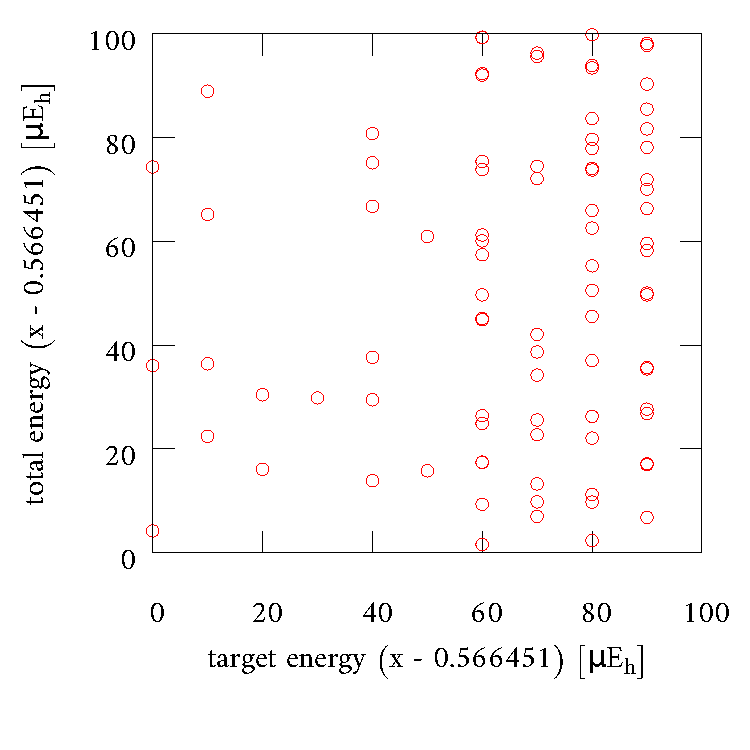
\includegraphics[width=0.5\textwidth]{Figures/E_k_benchmark}
%\caption{Energies of the solutions obtained for target energies varying in the $\mu\,E_h$-range.}
%\label{fig:E_k_bm}
%\end{wrapfigure}
%The obtained energies of the solutions vary strongly when changing the target momentum $k$ as the Figure \ref{fig:E_k_bm} illustrates.
%In the figure, the target energy is varied between $0.566451\,$a. u. and $0.066551\,$a. u. and lead to strongly changing eigenenergies.
%This strong dependence on $k$ is also observed when projecting the obtained FEFs onto spherical waves (\ref{eq:spherWave}) which is not shown here.

\section{Numerical Benchmarks and Stability Tests}
\subsection{Mesh-Construction and Quality}
\label{sec:NumConve}
In section \ref{sec:grid} several parameters for the setup of the grid were discussed whose numerical properties are te compared and evaluated in this section.
Here, three different schemes for distributing the concentric spheres are presented for the Lithium atom, each with a maximum radius $r_\text{max}=7\,$bohr and $N=20$ spheres.
In the scheme denoted in Table \ref{tab:RadScheme} and Figure \ref{fig:SchemHist} (left) as ``const'', the spheres are placed according to eq. (\ref{eq:tm_map}) with $N_i=74$ points on each sphere.
The scheme denoted as tm also uses eq. (\ref{eq:tm_map}) for the size of respective spheres but adapts the number of points per sphere according to (\ref{eq:tm_num}).
The last scheme tested here uses the radial mapping suggested by Son and Chu \cite{Son_Chu0} (\ref{eq:son_map}) and the number of points per sphere (\ref{eq:son_num}).
The parameters for the radial mapping are chosen as $l=1.8$ and $p=2.6$ and for the distribution of points on the spheres the Lebedev-scheme \cite{lebedev} is used, respectively.
\begin{table}
\begin{tabular}{|c|c|c|c|}
\hline
scheme & runtime [s] & DOS$^{a)}$ [$(m E_h)^{-1}$] & number of nodes\\
\hline
const   &  438   &    7    &   3255 \\
tm      &  825   &    13   &   5132 \\
son     &  891   &    4    &   6368 \\
\hline
\end{tabular}
\caption{The runtime, density of states and number of nodes used for the different radial mapping schemes that are described in the text.\\
$^{a)}$: density of states, averaged over 23 states}
\label{tab:RadScheme}
\end{table}
Some characteristic properties of the respective results are shown in Table \ref{tab:RadScheme}.
The runtime given in this table is only a rough estimation but seem to scale directly proportional to the number of nodes.
Seemingly the radial mapping scheme (\ref{eq:tm_map}) in combination with the angular density (\ref{eq:tm_num}) seems to be advantageous compared to the others even though it should be noted that this may be different for other parameters and that the density of states in these calculations is not uniform so that an average over more or fewer states can influence the results qualitatively.
However, the results may be very sensitive with respect to the change of parameters such as box-size and the parameter $l$, respectively.
Moreover, during the creation of tetrahedra from the given point-sets a quality-check is done by the respective library \cite{tetgen} which adds or removes points to ensure well-shaped tetrahedra which may, however, alter the distributions considerably.
These corrections of the point-set may be also responsible for the very similar distribution of the properties of the different tetrahedra.
In Figure \ref{fig:SchemHist} (left), the distribution of the ratio of the longest edge to the height of the smallest side is shown.
Here no significant differences between the schemes under investigation can be seen.

The angular distribution of points seems to be only of minor importance.
As shown in the Figures \ref{fig:SchemHist} and \ref{appFig:SchemHist} in supplement, the statistics are very similar and also the obtained density of states is very comparable.
However, the angular distribution can play a larger role when considering non-spherical systems.
In this work unless otherwise noted, the Lebedev scheme is used which provided the highest density of states (DOS) in this test.
The impression of very similar properties of the meshes generated by different schemes is also supported by the statistics of further parameters of the tetrahedra, see Figure \ref{appFig:SchemHist}.
\begin{figure}
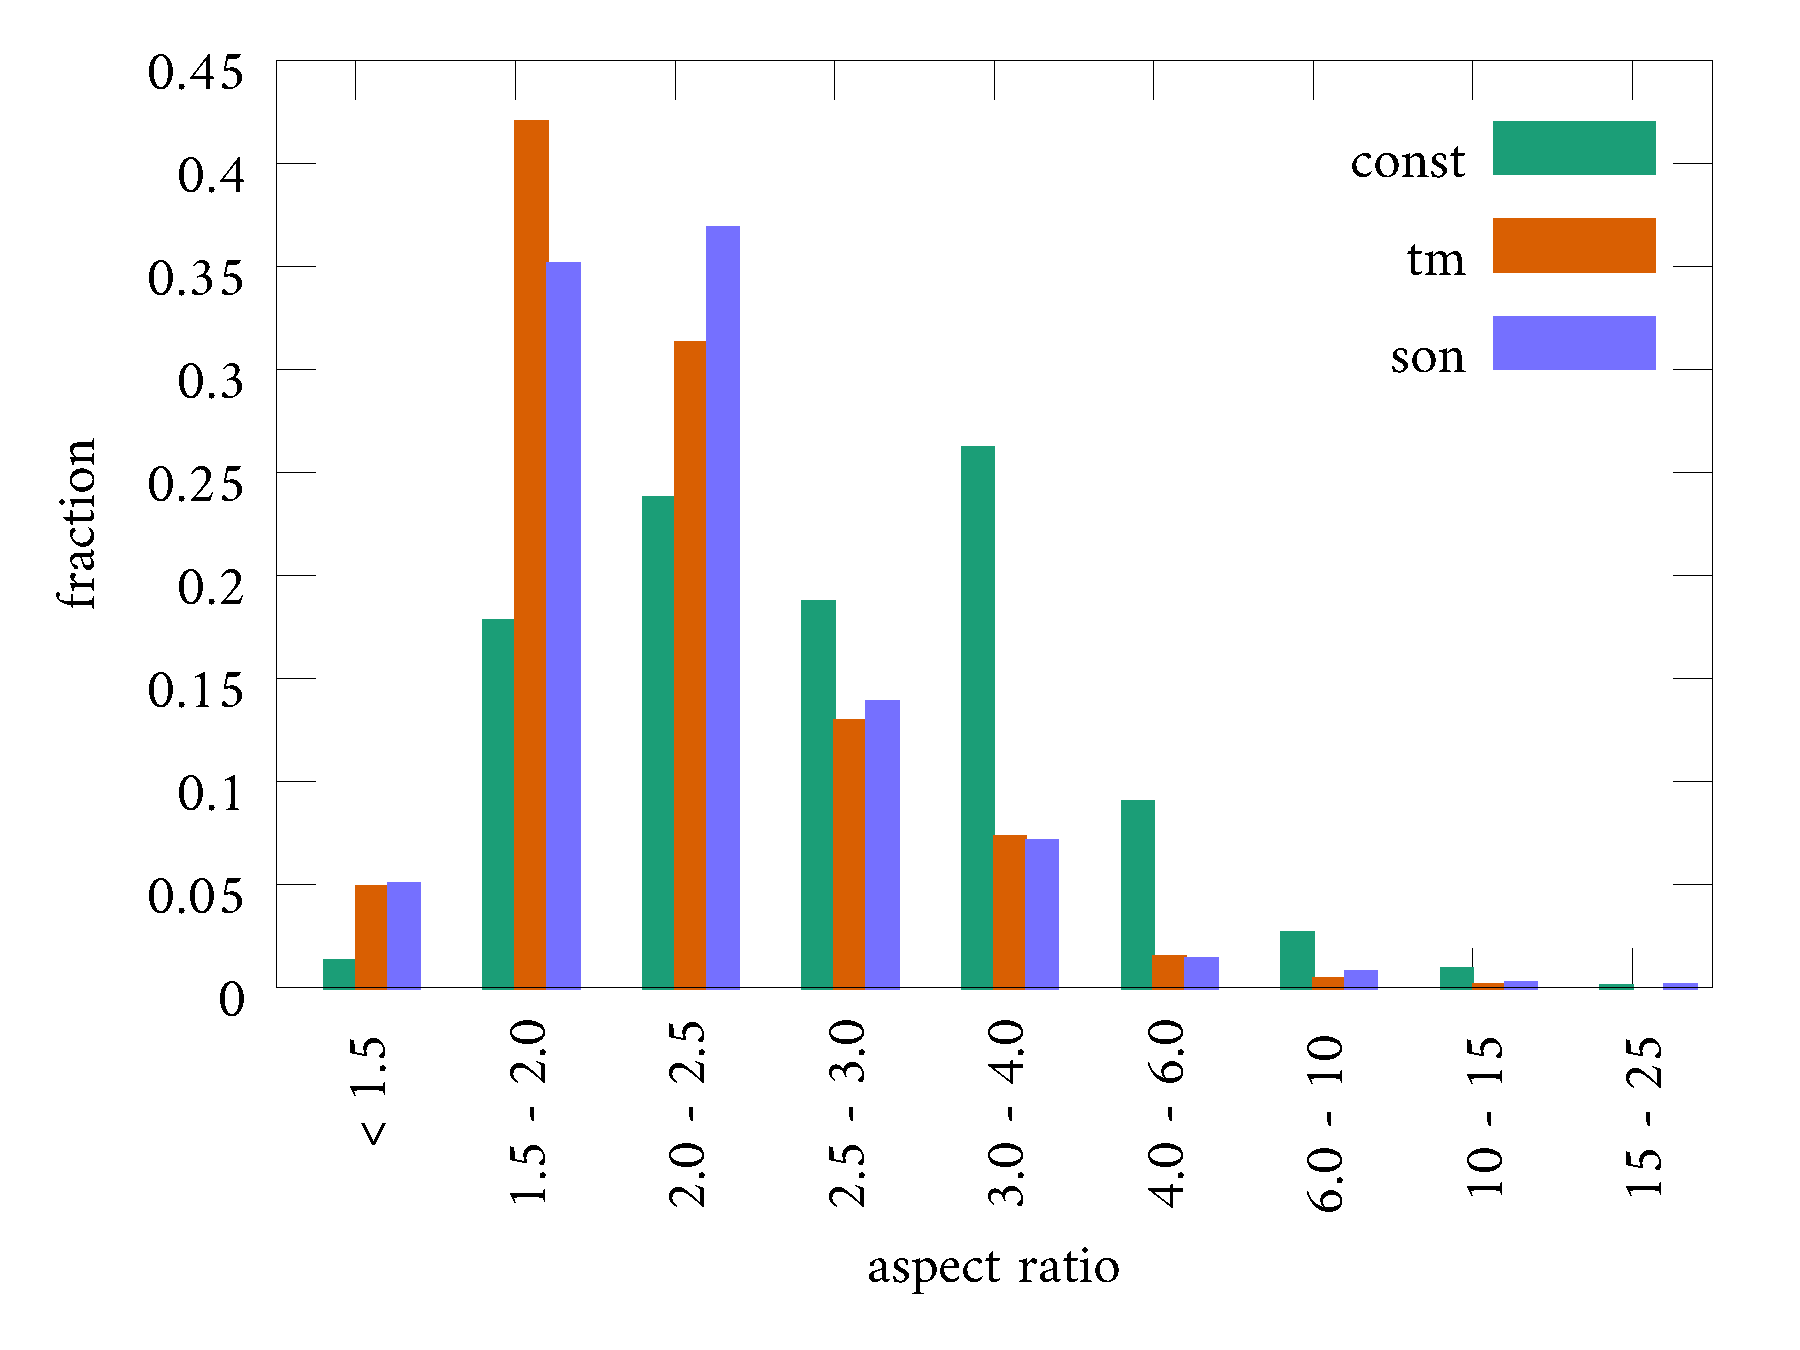
\includegraphics[width=0.49\textwidth]{Figures/Radi_hist.pdf}
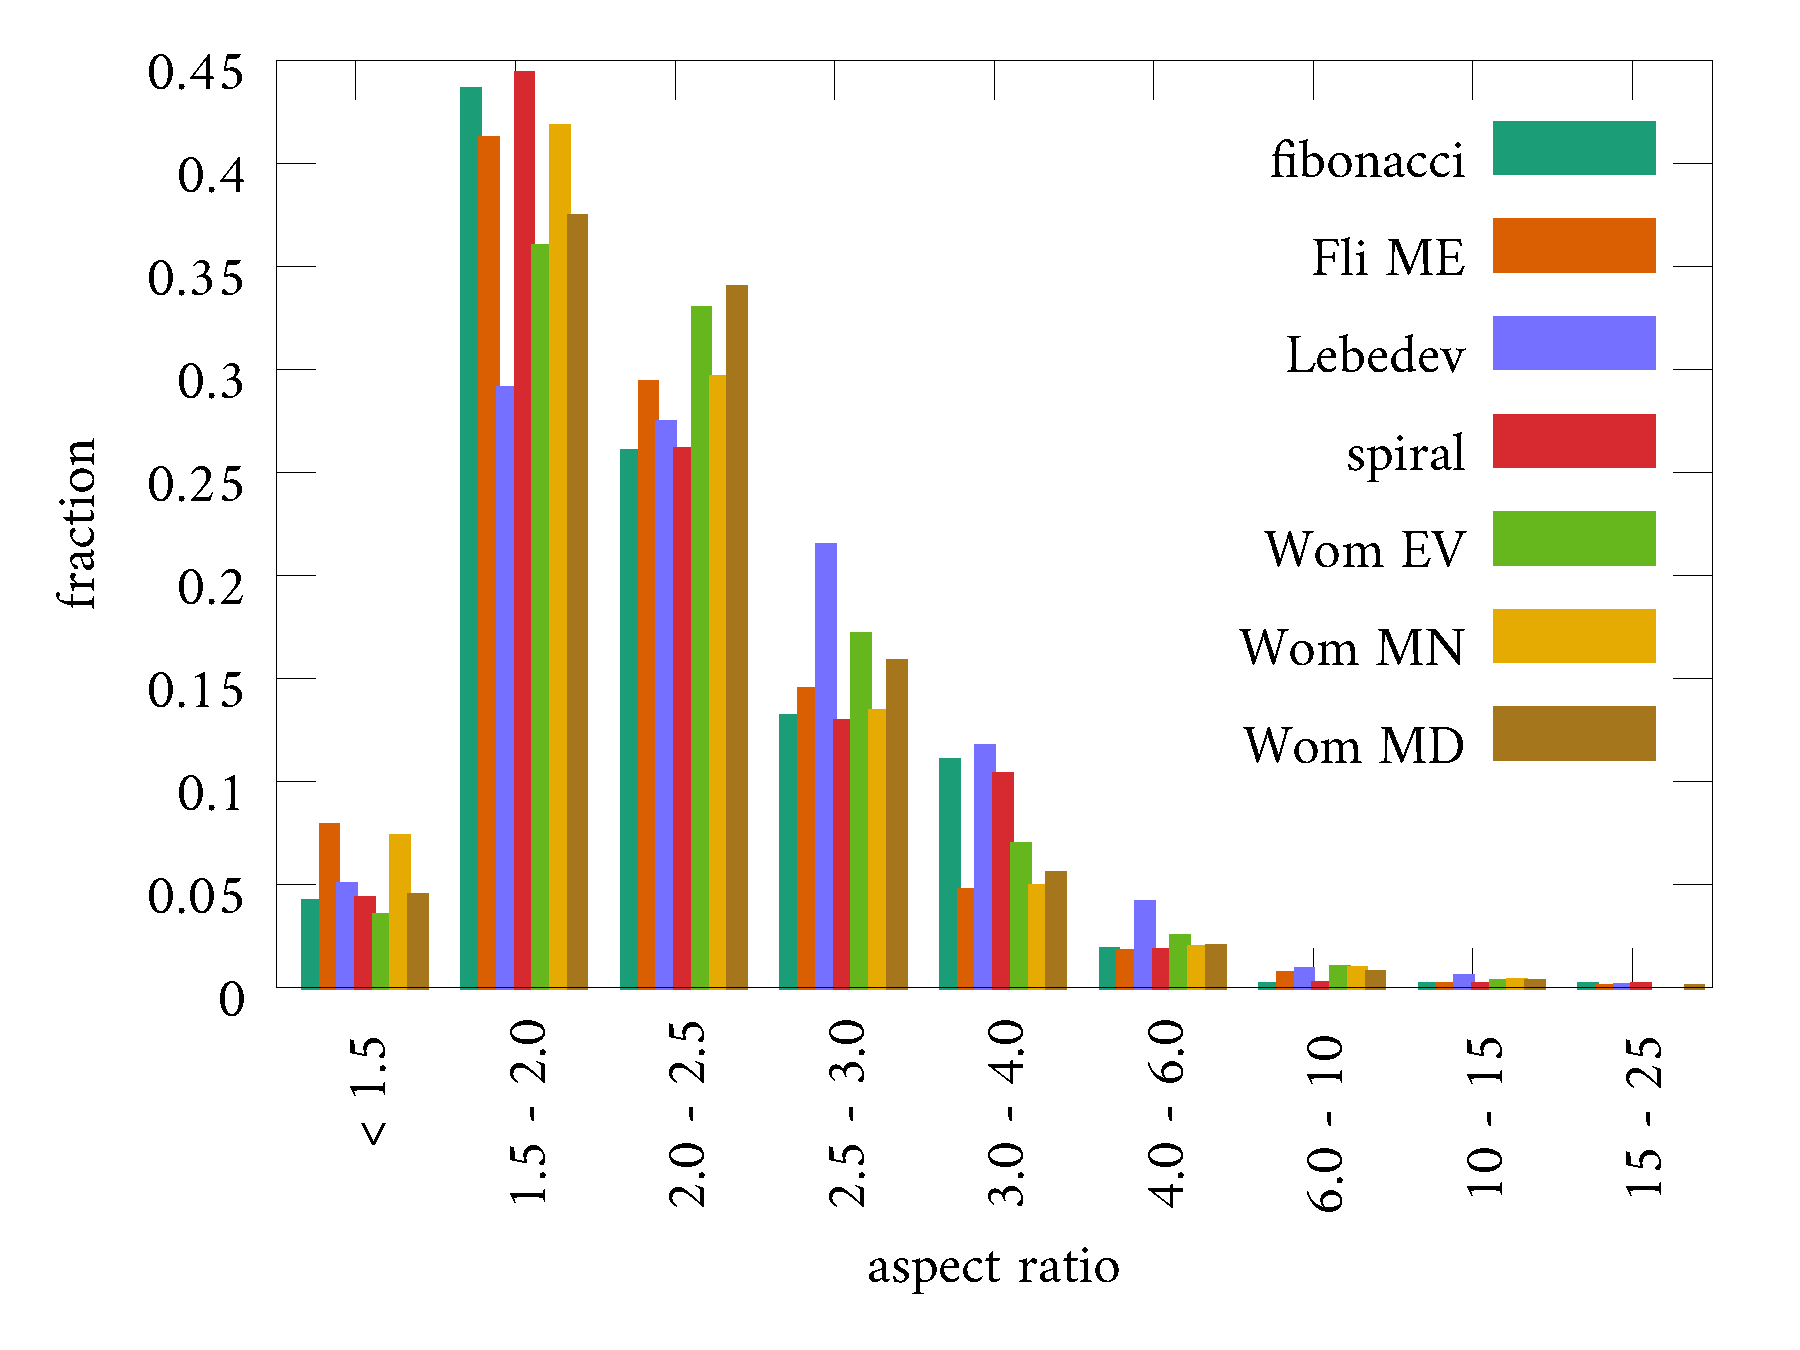
\includegraphics[width=0.49\textwidth]{Figures/Sph_hist.pdf}
\caption{Distribution of aspect ratio (longest edge length divided by the smallest side height).
   Be aware that the ranges of the different bins differ.}
\label{fig:SchemHist}
\end{figure}
Concluding one can say that the procedures studied here yield meshes with similar quality.

\subsection{Numerical Convergence}
In the FEM scheme used to compute the FEF, several parameters governing numerical and physical characteristics are used such as box-size, target energy and subspace used for solving the eigensystem.

The size of the Krylov-subspace does not play a role for the quality of the solution as shown in Figure \ref{fig:E_nev} for the symmetric formulation with a power $p=\frac 12$ of the damping function $D$.
\begin{wrapfigure}{R}{0.5\textwidth}
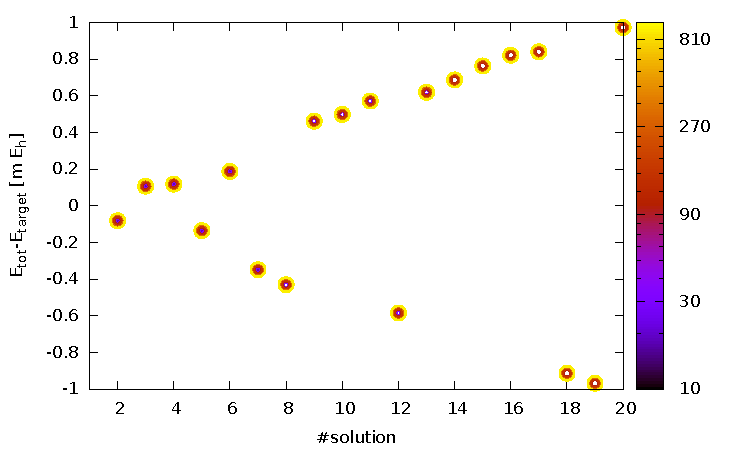
\includegraphics[width=0.5\textwidth]{Figures/Root_E_nev.pdf}
\caption{The energies of the 20 states that fit the target energy best, depending on the
size of the Krylov-suspace, indicated by the colour.}
\label{fig:E_nev}
\end{wrapfigure}
Such a good behaviour can, however, only be observed for the symmetric case because in case of the non-hermitian formulation the ordering of the eigenvalues can not be done unambiguously.

\section{atomic Lithium}
\label{ch:resLI}
As the smallest system that has multiple electrons in its anionic state as well, Lithium is a good test object that has theoretical as well as experimental reference data available, \cite{Li-R,Li-R1, LiNaRef1} even though its appearance in a work on `complex molecules' might surprise.
However, its photoelectron spectrum consists, except for a single valence peak, only of the core electron spectrum.
In this region the estimated binding energies are often not that good as those obtained for valence orbitals and, moreover, two out of four main peaks of the spectrum arise due to dipole-transitions in the bound part and thus are not accounted for due to the neglect of the conjugated Dyson orbital in eq. (\ref{eq:fullDO}) \cite{saPonzi}.
%The appearance of $2p$-states are accessed by a dipole-transition in the bound part and can not be described within the theory applied here due to the neglect of the conjugate DO term in equation (\ref{eq:fullDO}) \cite{saPonzi}.
%Experiment from Moore, cited in \cite{LiNaRef1}; original not found.
%Experiment 2 from \cite{LiSonntag}.
%
%\begin{wrapfigure}{l}{0.7\textwidth}
%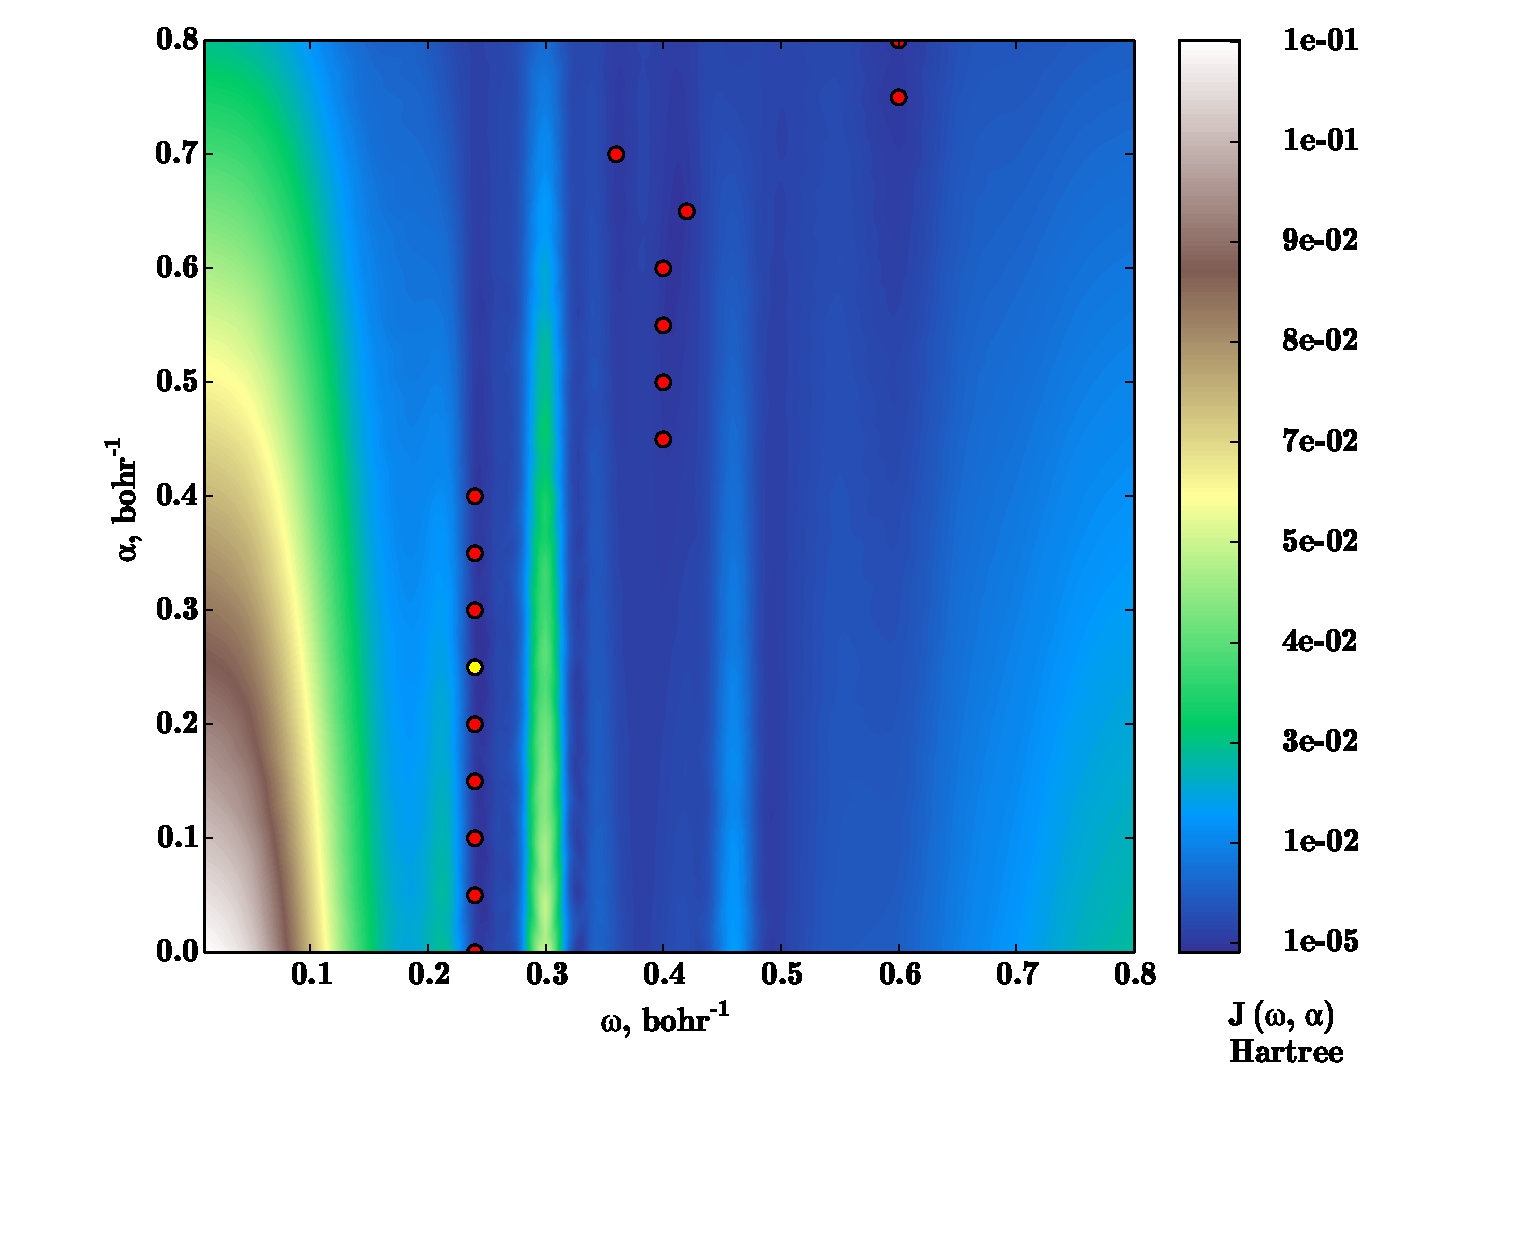
\includegraphics[width=0.69\textwidth]{Figures/Lithium/Lithium_J0_2D_terrain_path_spline_cut}
%\caption{The functional $J(\alpha,\omega)$ described in eqation (\ref{eq:J_ao}) for Lithium}
%\label{fig:Lith-otrsh}
%\end{wrapfigure}

However, the well-separated single valence peak allows a more detailed study of the photon energy dependence of the intensity of a single peak as shown in Figure \ref{fig:Li-CS} where experimental values are compared with several theoretical models.
% TODO: this figure in supplement to show comparison with other theoretical results?
%\begin{wrapfigure}{l}{0.7\textwidth}
%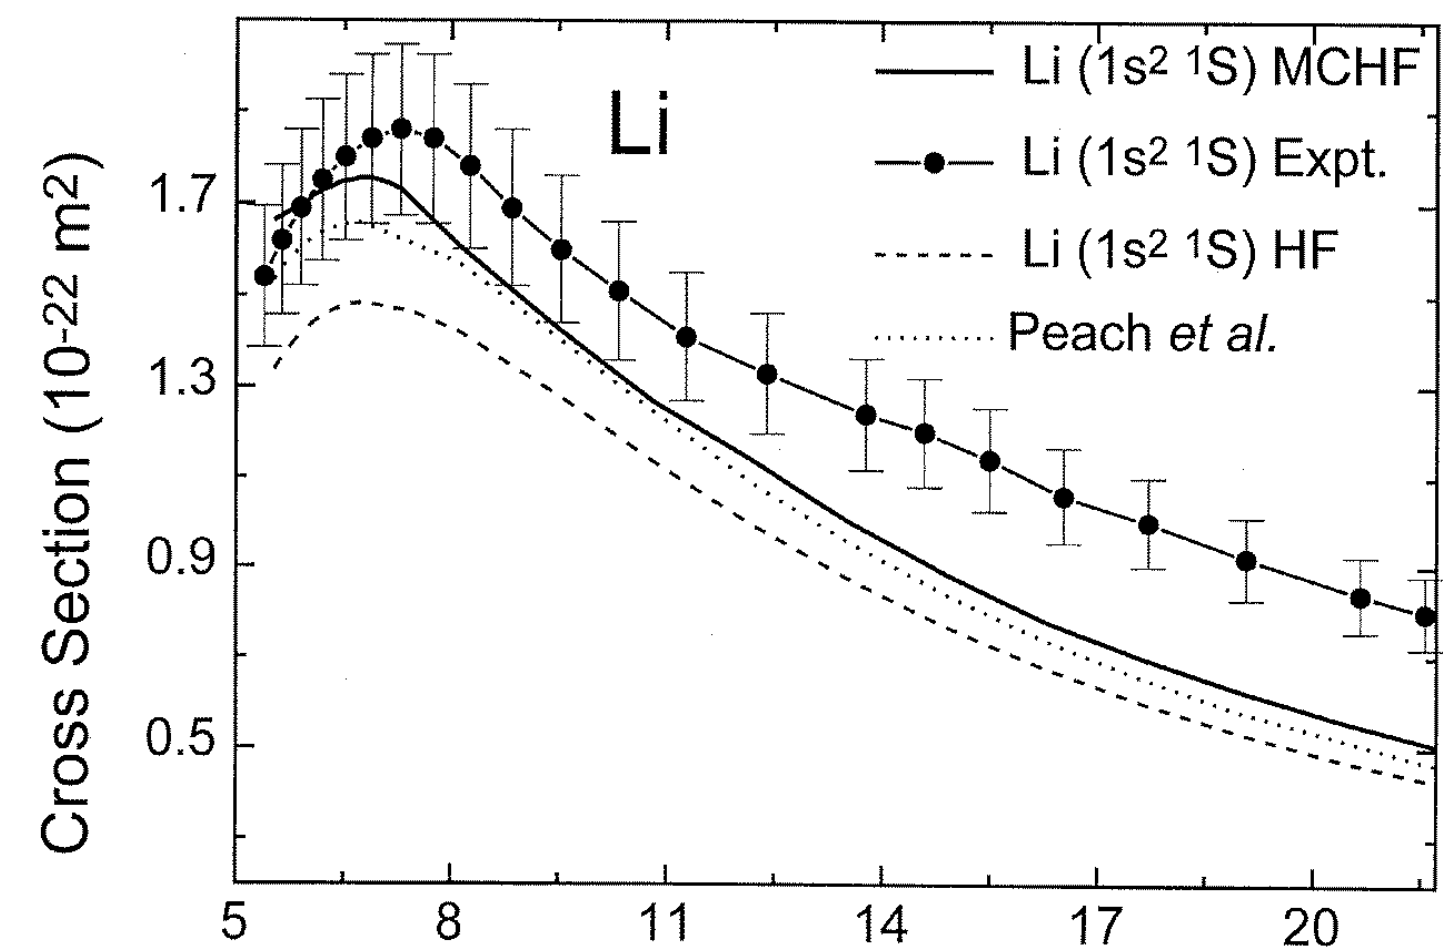
\includegraphics[width=0.69\textwidth]{Figures/Lithium/Li_crossSect}
%\caption{Cross section of the Lithium atom as function of the photon energy \cite{LiCS}.}
%\label{fig:Lith-cs}
%\end{wrapfigure}
\begin{figure}
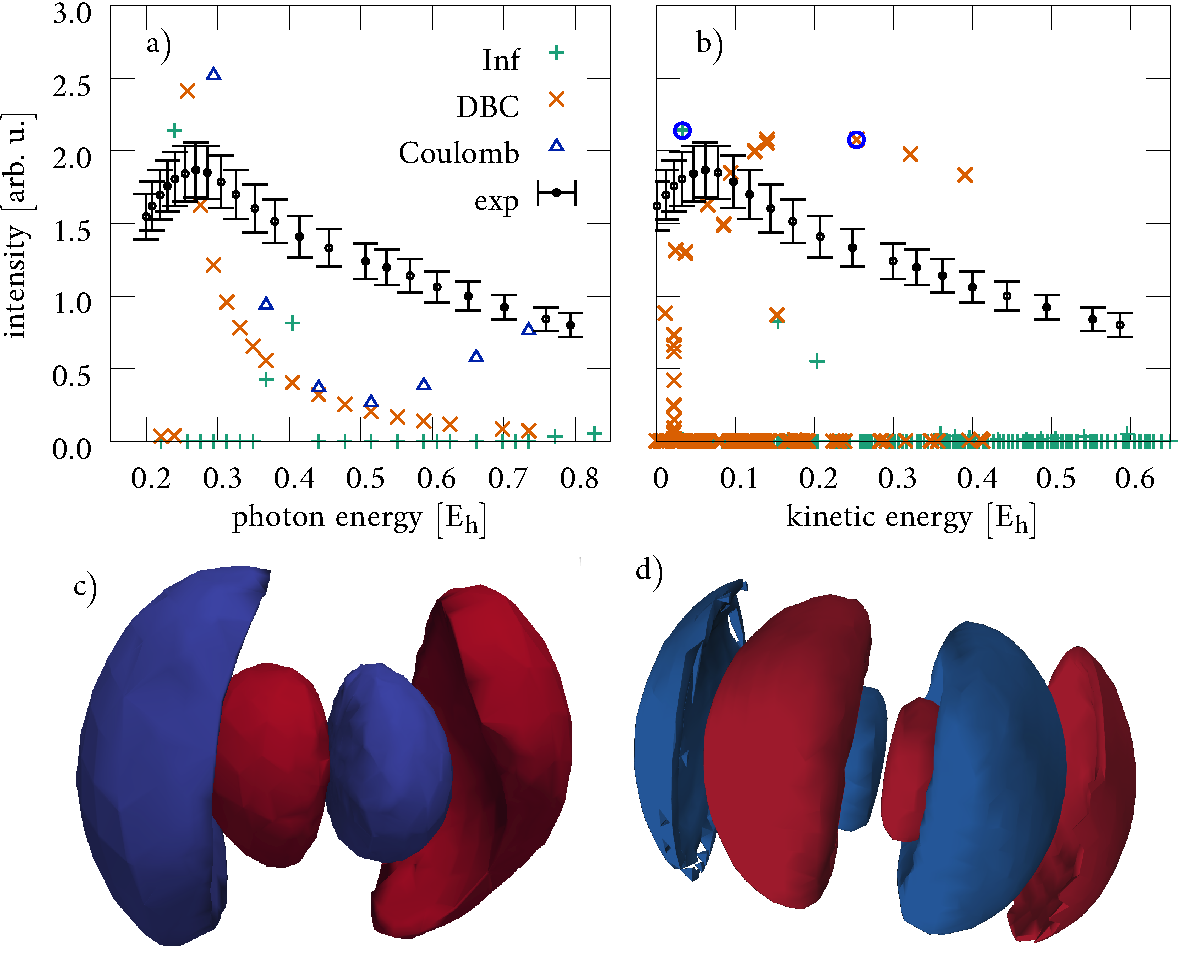
\includegraphics[width=\textwidth]{Figures/Lithium/CrossSect2}
\caption{The photoelectron cross section of the Lithium atom as a function of the photon energy obtained with Dirichlet BCs (DBCs) and with infinite elements (inf), compared to experiment  \cite{LiCS}.
In the left panel, the intensity is the sum over intensities for $80$ FEFs respectively, in the right panel the intensities of single functions are shown.}
\label{fig:Li-CS}
\end{figure}
Since the protocol developed in this work does not provide absolute cross sections, the results obtained here are scaled to fit the reference data best.
Moreover, it was shown in chapter \ref{ch:bmSize} that the size of the FEM-region plays an important role for the nature of the obtained solutions but no conclusive scheme for a reasonable choice for the radius has been given so far.

%\section{Triatomic Linear Molecules}
\section{CO$_2$}
As a second test-system, CO$_2$ is a
There are several studies on CO$_2$ \cite{CO2, CO2_highres, HighResLinear, DiffLinear},
% CS$_2$ \cite{DiffLinear,HighResLinear}, COS \cite{DiffLinear,HighResLinear} and N$_2$O \cite{DiffLinear}
%CS$_2$ is known to have strong correlation effects \cite{2phcederbaum}
\begin{wrapfigure}{R}{0.6\textwidth}
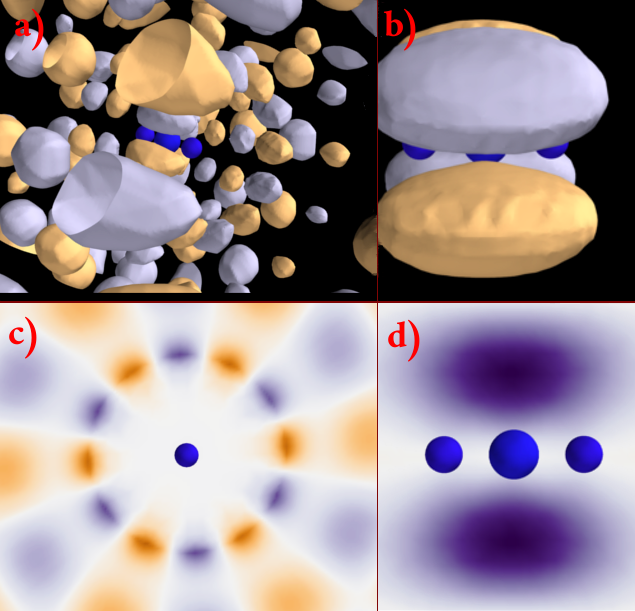
\includegraphics[width=0.6\textwidth]{Figures/CO2/Solutions}
\caption{Free electron functions obtained with infinite elements (left) and with Dirichlet boundary conditions (right)}
\label{fig:CO2_exs}
\end{wrapfigure}

\begin{wrapfigure}{L}{0.7\textwidth}
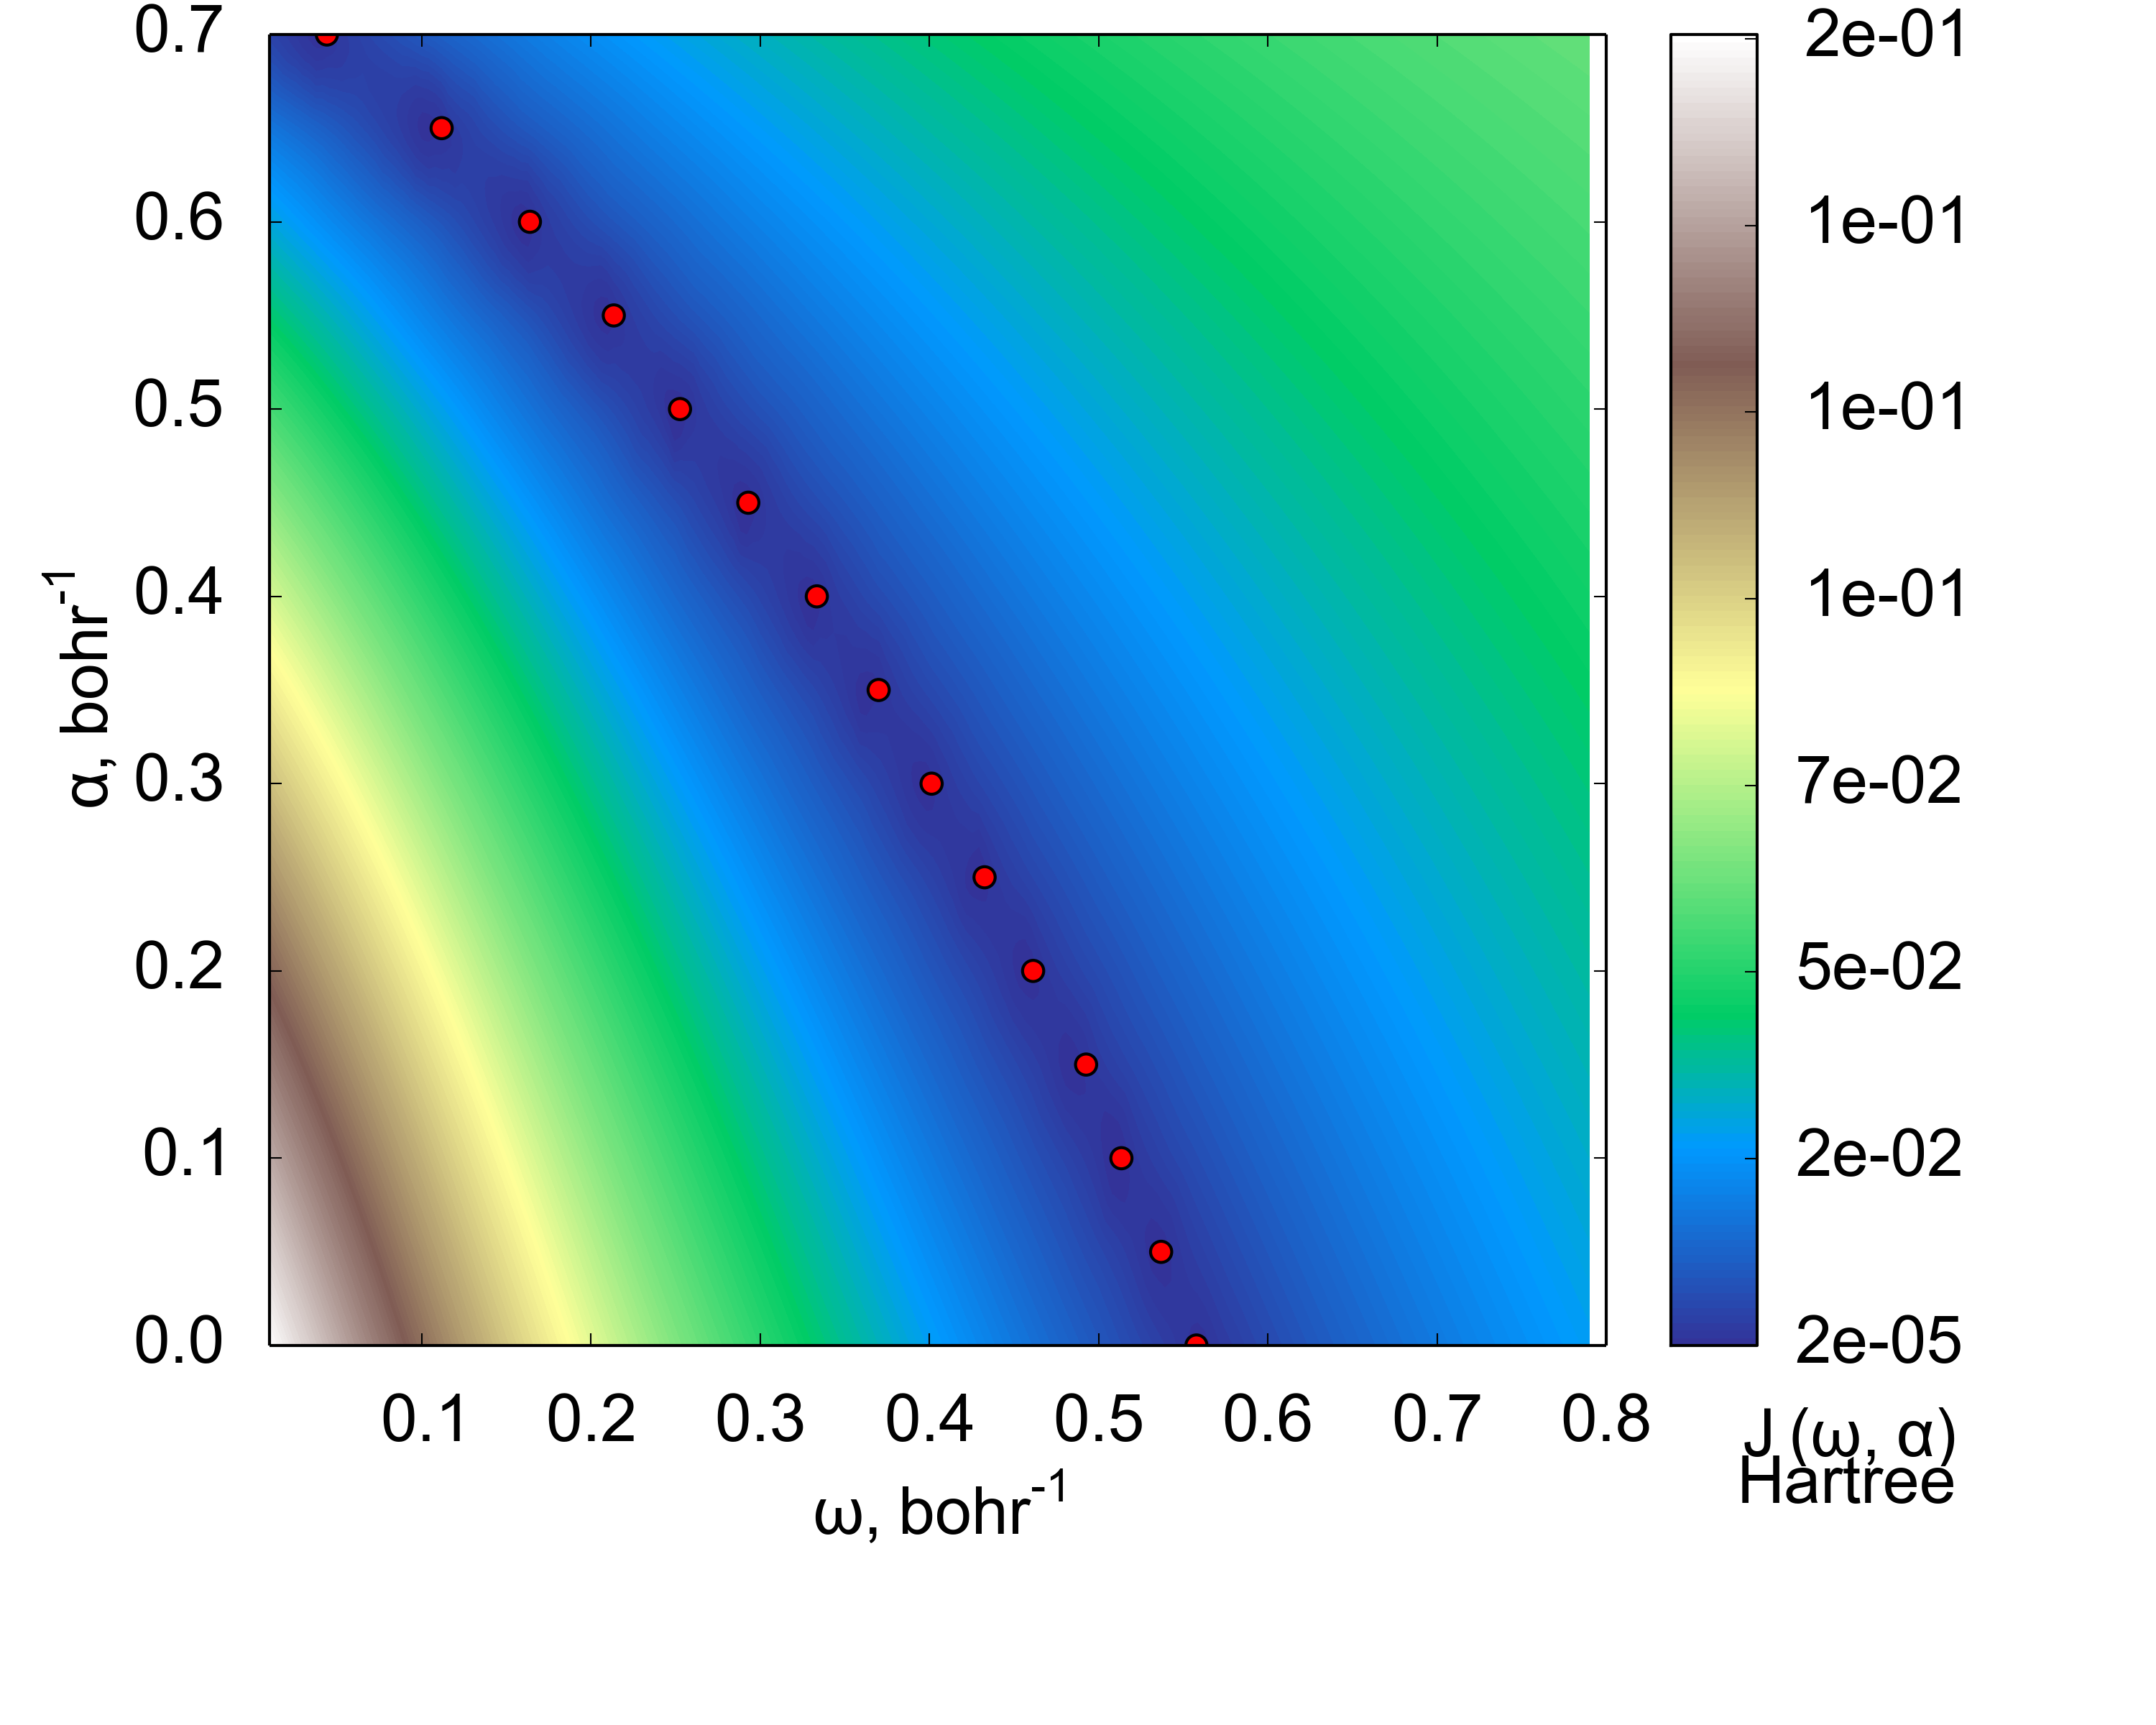
\includegraphics[width=0.69\textwidth]{Figures/CO2_J0_2D_terrain}
\caption{The functional $J(\alpha,\omega)$ described in eqation (\ref{eq:J_ao}) for CO$_2$}
\label{fig:CO2-otrsh}
\end{wrapfigure}

Cross-section profiles of CO$_2$ in \cite{stieltje}.

Data of CO2: \cite{DiffLinear}.

\section{water}
The PES and threshold PES, where the kinetic energy of the photoelectron is kept constant instead of the energy of the photon, of water is experimentally well studied 
for different photon energies.
As example, in Ref. \cite{waterTPE} the PES of water and several TPES of water and heavy water are investigated with high resolution.\\
Similar high accuracy is achieved in Ref. \cite{waterHePES} where the PES of H$_2$O$^+$ and D$_2$O$^+$ are studied with a He1 source, radiating at $537\,$Angs.\\
Further PES are available at higher photon energies:
In \cite{water1200}, photons at energies of $1200\,$eV are used.
A further study of Winter \textit{et. al.} measured spectra at $60$, $75$ $80$, $100$ and $120\,$eV in gas and liquid phase \cite{winterWater}.\\
These studies are of interest here since they yield a variety of different test-cases on a single system that can be used to prove the method being used to be valid.


\chapter{Resumee}

\subsection{Boundary condition}
The dependence of density of eigenenergies to size/mixing of angular momenutum can also hold for the different formulations of infinite elements, compared in section \ref{ch:bmFormul}, as well.
Thus, a comparison of the different formulations could be redone under this aspect, probably leading to better results.
However, previous studies that are not presented in this work have shown that the Astley-Leis elements leads to similar problems which initially motivated the symmetric formulation.

 - is it worth the effort?
 - What energy-range is achievable?
 - Which effects are still missing?

 - How to proceed with it?


%\renewcaptionname{english}{\abstractname}{Acknowledgement}
%\begin{abstract}
\newpage
\section*{Acknowledgement}
1.: Sergey\\
2.: Gilbert\\
3.: Olga\\
4.: K\"uhn
%\end{abstract}

%\nocite{*}
\small{
\printbibliography
}

\appendix

\chapter{Appendix}
%\input{appendix_do}
%\section{Finite elements}
%\input{appendix_fem}
%-- general rules:\\
%   -> dependence of intensity on $E_kin$ (\cite{Gao_wopperer} for num. study) 
%     Is there some? \\
%
%\section{Iteratively Solving Sparse Generalised Eigenproblems}
\label{app:ghep}

\subsection{Lanczos-schemes}

\section{Regularisation of Eigenvalue problems}
\label{app:regular}

\section{Additional Data}

\begin{wrapfigure}{r}{0.7\textwidth}
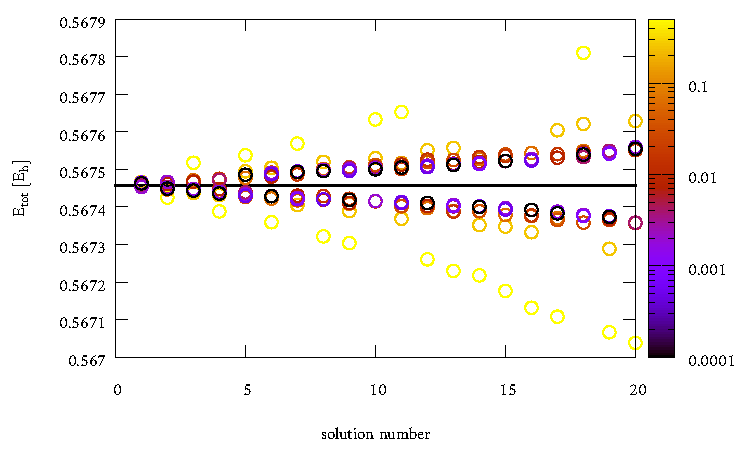
\includegraphics[width=0.7\textwidth]{Figures/IFem_powers_spectra}
\caption{The eigen energies of the first 20 solutions (circles) for different powers $p$ of the damping function $D(r)$ which determines the colours.
The spectra do not change significantly for $p<\frac 18$.}
\label{fig:powerSpect}
\end{wrapfigure}


%%\section{Delaunay Triangulation}
%\label{app:delaunay}
%The explicit setup of non-regular meshes for the use in finite element schemes is not trivial at all.
%There are however schemes available, among which are the Delaunay and Voronoi tesselations which are their respective dual schemes.
%Since in this thesis, only Delaunay tesselation is used, I will focus on this method and its properties only.\\
%%In mathematics one understands under a triangulation a connection of points to simplices.
%Thereby a structure is denoted as a simplex in $n$ dimensions, if has as few vertices as possible in this dimension.
%A simplex in $2D$ \textit{e.g.} is a triangle while it is in $3D$ a tetrahedron.
%Moreover, a simplex is denoted as Delaunay simplex if there is a circumsphere such that no vertex is inside of this sphere.\\
%A bit more intuitive acess to this scheme can be obtained via the Voronoi diagram: A Voronoi diagram splits a given volume (in $3D$) into elements using a set of points $p_i$ in this volume by assigning each point to the element of his nearest point $p_i$.
%Having this tesselation, one can transform it to a set of Delaunay simplices by connecting the points $p_i$ each with their direct neighbours \cite{tetgen}.

\newpage
\section*{Selbst\"andigkeitserklaerung}
Ich versichere hiermit an Eides statt, dass ich di vorliegende Arbeit selbstst\"andig und ohne fremde Hilfe verfasst habe, keine au\ss er den von mir angegebenen Hilfsmitteln und Quellen dazu verwendet habe und die den benutzten Werken inhaltlich und w\"ortlich entnommenen Stellen als solche kenntlich gemacht habe.

\vspace{20mm}
\hfill Rostock, \date
%\printindex
\backmatter
\end{document}
